\chapter{绪论}\label{sec:绪论}

现代医学成像技术为人类探索自己的大脑提供了一个前所未有的非侵入式的观察与研究的机会。这些成像技术包括数字X射线摄影(Digital Radiography, DR)、X 射线计算机断层成像(X-Ray Computer Tomography, CT)、超声成像(Ultrasonic Imaging, UI)、正电子发射型计算机断层成像(Positron Emission Tomography, PET)、磁共振成像(Magnetic Resonance Imaging, MRI)等\cite{picano2004sustainability}。在这些技术中,MRI由于其较高的图像分辨率,对于组织中水含量变化的敏感性,较强的软组织分辨能力以及无放射性危害等特点,被广泛地用于人类大脑结构成像(structural MRI, sMRI)与功能成像(functional MRI, fMRI)\cite{giedd1999brain},由此得到的清晰的大脑结构图像与功能图像不仅可以测量评价大脑的很多生理指标,例如灰质体积、白质体积、皮层厚度、大脑不同区域的功能连接等,还可以进一步推导相应的功能认知过程\cite{poldrack2006can}。因此,在最近几十年中,MRI被越来越多地用来研究神经系统发育,例如人类脑连接计划(Human Connectome Project, HCP)\cite{van2013wu}、婴儿脑连接计划(Baby Connectome Project, BCP)\cite{howell2019unc}、发育脑连接发育计划(developing  Human Connectome  Project,  dHCP)\cite{makropoulos2018developing}等,以及用来诊断神经系统疾病,例如阿尔茨海默病(Alzheimer's Disease, AD)\cite{mueller2005alzheimer}、帕金森病(Parkinson's Disease, PD)\cite{brooks2003assessment}、自闭症\cite{anagnostou2011review}等。

经过几十年的发展,处理与分析这些大脑MRI数据已经形成了一个完整成熟的流程(pipeline)\cite{glasser2013minimal,li2019computational}。一般来讲,大脑sMRI数据处理流程(Structure MR images processing pipeline)主要包含两部分:(1)基于脑体积的分析(Volume-based Analysis),(2)基于脑皮层表面的分析(Surface-based Analysis),如图\ref{fig:flowchart_of_MRI_process_pipeline}所示。其中基于脑体积的分析一般指基于2D/3D的大脑MR图像的影像定量分析,提供大脑相关生理指标,例如形状、大小、体积以及纹理特征等。随后利用机器学习技术探索并分析这些特征,为诊断、预后或预测提供有价值的信息,从而开发诊断、预测或大脑发育的模型。基于大脑皮层表面的分析则更好地利用了大脑皮层的2D拓扑属性,可以更方便、更准确地映射和绘制大脑,从而更好地捕捉动态复杂的皮层上的神经生物学变化。MRI数据处理pipeline中的这两种方法在过去十几年中不断发展,相互结合,相互帮助,为我们理解大脑发育、诊断与治疗神经系统疾病提供了很好的工具与手段,也为神经影像学、脑科学和生命科学带来了新的发展机遇以及很多新的发现。例如,基于脑体积的分析揭示了阿尔茨海默病的大脑灰质的萎缩现象,并进一步发现了这种萎缩现象会随时间从颞叶扩散到额叶和枕叶大脑区域\cite{thompson2003dynamics},为AD的临床诊断提供了可靠的支持。基于大脑皮层表面的分析在婴幼儿的大脑发育中也帮助发现了很多早期脑发育的奥秘\cite{li2019computational,wang2019developmental,duan2019exploring}。

\begin{figure}[t]
    \centering
    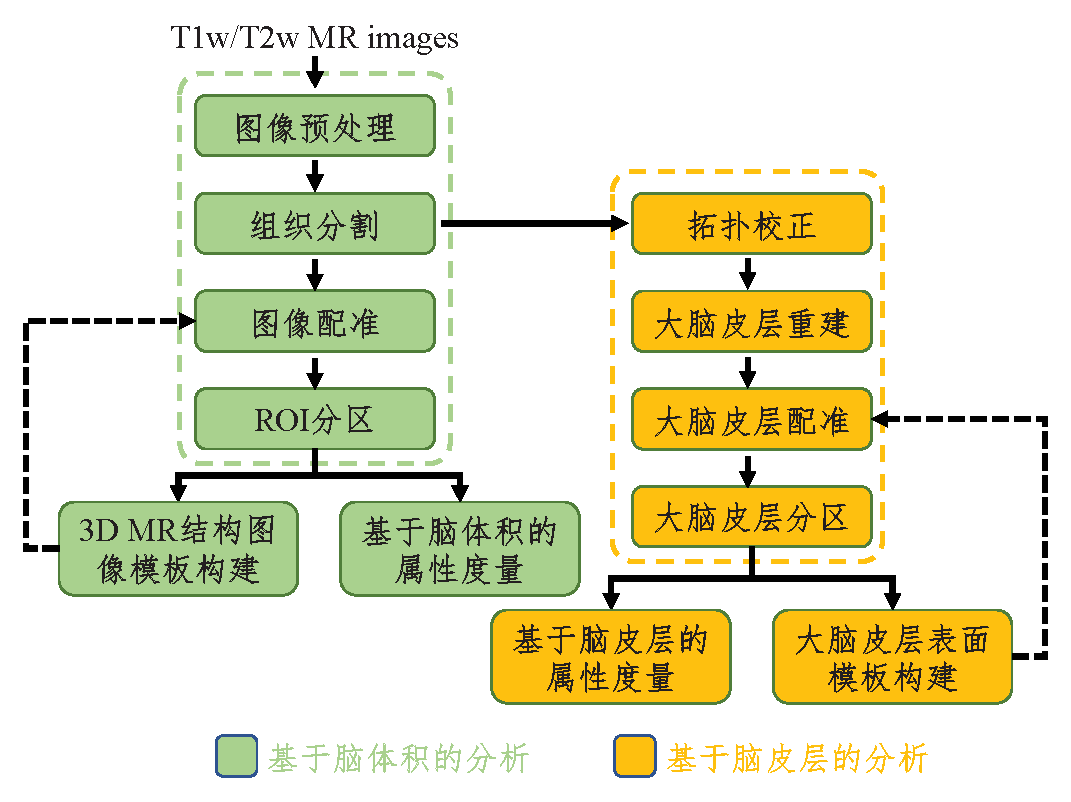
\includegraphics[width=.8\linewidth]{figure/flowchart_of_MRI_process_pipeline.eps}
    \caption{\label{fig:flowchart_of_MRI_process_pipeline}典型的结构MR图像处理流程。其中橙色标记的基于脑皮层表面的数据处理与分析即是本论文所要研究的内容。}
\end{figure}

近几年来,得益于高计算力的计算机显卡(GPU)的强大计算能力,以及卷积神经网络(Convolutional Neural Network, CNN)的强大学习能力,深度学习技术\cite{goodfellow2016deep}在很多领域都取得了非常好的结果。这一方面是计算力提升的结果,另一方面也得益于卷积计算的优秀图像特征提取能力。通过合适的建模与训练方法,我们可以得到一个合适的CNN模型用来拟合大多数计算机视觉或医学图像处理领域中的任务,例如分类、分割、检测、目标追踪等。目前,CNN在图像处理中已经全面优于各种传统的特征提取加上机器学习的方法,在医学图像处理领域的应用也越来越多,都展现了非常优越的性能\cite{shen2017deep,litjens2017survey}。在大脑MRI数据处理pipeline中,很多深度学习技术也被用到了基于脑体积的分析中\cite{li2019computational}。这些方法显著提高了大脑MRI数据处理pipeline的效率、准确率以及自动化率,使得大规模多中心的脑影像数据分析成为可能。但是,另一方面,基于脑皮层的分析大多还使用传统的机器学习与计算方法,甚至时常还需要人工专家的介入,深度学习方法依然很少见或不实用。这使得基于脑皮层的处理与分析成为了拖累整个大脑MRI数据处理pipeline的短板部分。

因此,为了解决这个问题,本论文将主要探讨怎样将深度学习技术更加方便准确地应用到大脑皮层表面数据的处理与分析上,希望能够借助深度学习的力量推动神经影像学研究在大脑皮层分析方向上的进步与发展。为了对上述所提及的大脑结构MR图像处理流程与基于脑皮层的数据处理与分析有一个更加全面与直观的了解,我们将在下一节详细介绍他们的背景、意义与研究现状。

\begin{figure}[h]
    \centering
    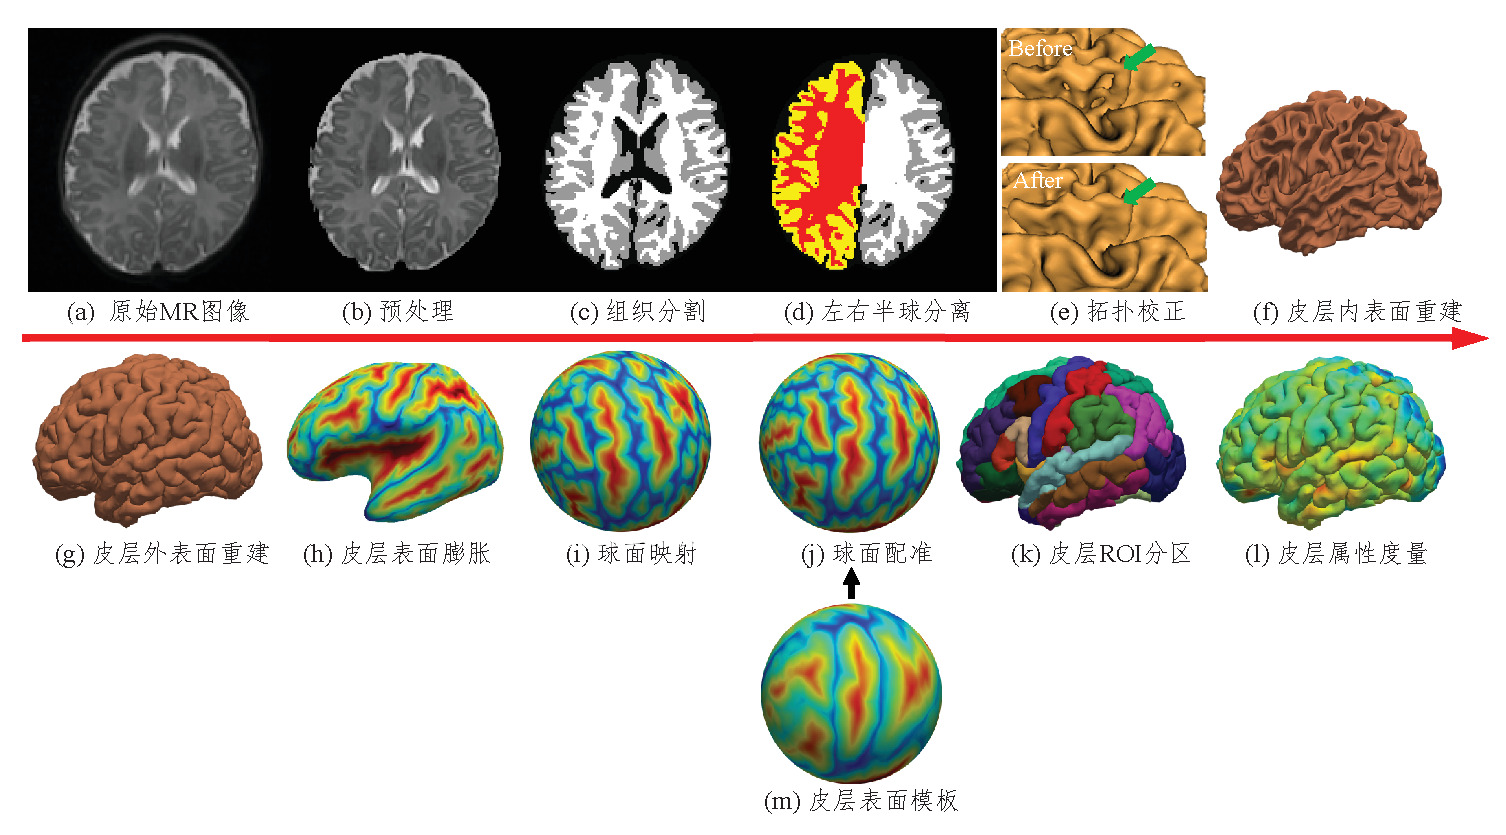
\includegraphics[width=\linewidth]{figure/flowchart_of_surface_based_analysis.eps}
    \caption{\label{fig:flowchart_of_surface_based_analysis}典型的基于大脑皮层的数据处理与分析流程}
\end{figure}

\section{大脑皮层表面的重建及其意义}
正如在图\ref{fig:flowchart_of_MRI_process_pipeline}中所展示的那样,MRI数据从图像到大脑皮层表面的重建有一套完整的流程。图\ref{fig:flowchart_of_surface_based_analysis}展示了一个更加直观完整的基于脑皮层的处理与分析流程。它主要分为三个阶段,(1)MR图像预处理,包括头动校正,头骨、小脑及脑干的去除,灰度不均匀校正,图像配准,灰质、白质及脑脊液的组织分割;(2)皮层表面重建,包括给非皮层结构施加掩模并进行填充,大脑左右半球分离,拓扑错误校正,皮层内表面重建,皮层外表面重建,以及皮层表面各种特征的计算;(3)基于皮层表面的处理与分析,包括球面映射,球面配准,感兴趣区域(Region of Interest, ROI)的分区,皮层表面重采样及各种皮层特征的重采样。这一小节我们将详细地介绍如何进行这每一步的操作来得到最终重建好的大脑皮层表面,并在下面几个小节介绍后续的基于皮层表面的处理与分析。

\subsection{MR图像预处理}\label{sec:MR图像预处理}
要采集到高质量的MR图像,第一步要做的就是头动校正\cite{zaitsev2015motion}。由于人体在采集过程中的不规则运动,MR图像很容易出现运动伪影,如重影、模糊、对比度变化或信号间隙等。为了减少运动伪影,目前最常用的有先进的回顾性的\cite{atkinson1999automatic},前瞻性的\cite{zaitsev2006magnetic}及混合的\cite{aksoy2012hybrid}扫描技术。

第二步,头骨剥离,用来保留脑实质而去除非脑组织部分。非脑组织包括颅骨、头皮和硬脑膜等。因为婴儿的MR图像比成人的图像分辨率低,且图像灰度、脑大小和形状会随着发育过程动态变化,所以现有的头骨剥离方法可以分为两大类,即用于成人的和专门用于婴儿的。成人的头骨剥离方法有很多,例如成熟的FreeSurfer\cite{fischl2012freesurfer}、fsl\cite{jenkinson2012fsl}、基于图割(graph cut)的方法\cite{sadananthan2010skull},基于水平集(level-set)的方法\cite{zhuang2006skull},基于3D U-Net的方法\cite{hwang20193d},等等。更多的最新的方法可以在这篇综述中找到\cite{kalavathi2016methods}。而专门用于婴儿的大脑MR图像头骨剥离的方法就比较少了。Mahapatra等人\cite{mahapatra2012skull}曾使用图割框架并结合先验形状信息,提出了一种针对新生儿的头骨剥离方法,并在20例新生儿的图像上做了验证。Shi等人\cite{shi2012label}提出了一种基于学习的脑提取和标记的算法。Zhang等人\cite{zhang2019frnet}利用卷积神经网络与残差连接来进一步提升婴儿大脑MR图像的头骨剥离的效果。由于其优越的性能,目前已被广泛地应用于婴儿脑连接计划项目(BCP)中。

第三步,灰度不均匀校正\cite{belaroussi2006intensity}。灰度不均匀是指由于射频线圈不均匀性和磁场不均匀性\cite{vovk2007review}导致的MR图像上随机变化的信号强度。因为大脑MRI处理算法,例如图像分割、配准等,会假设在每个组织内灰度均匀,所以灰度不均匀会极大地降低这些算法的性能。目前,广泛使用的灰度不均匀校正的方法是非参数不均匀灰度归一化(Non-parametric Non-Uniform Intensity Normalization, N3)\cite{sled1998nonparametric}和它的改进版本,N4算法\cite{tustison2010n4itk},也有一些研究将其整合进组织分割过程中\cite{wang2011automatic}。

第四步,图像配准\cite{sotiras2013deformable}。配准是指将每个个体的图像映射到一个公共的模板空间,从而使不同个体的同一大脑位置一一对应起来。医学图像配准最经典的方法有fsl的FLIRT\cite{jenkinson2001global,jenkinson2002improved},FreeSurfer\cite{fischl2012freesurfer},ANTs(Advanced Normalization Tools)的SyN\cite{avants2008symmetric},以及最近几年基于深度学习的无监督网络\cite{dalca2018unsupervised,balakrishnan2018unsupervised,niethammer2019metric,de2019deep}等。

第五步,组织分割,旨在将大脑MR图像分割成三种不同的组织类型,即灰质(Gray Matter, GM)、白质(White Matter, WM)与脑脊液(Cerebrospinal Fluid, CSF)。这一步是定量研究大脑神经系统发育与病变的重要步骤。有很多成熟的工具软件可以直接用于成人大脑的分割,如FSL\cite{jenkinson2012fsl}、FreeSurfer\cite{fischl2012freesurfer}、SPM\cite{tzourio2002automated}和BrainSuite\cite{shattuck2002brainsuite}。由于婴儿大脑MR图像的灰度与对比度比成人脑图像低很多,研究人员开发了专门针对婴儿脑图像的分割算法\cite{li2019computational}。现在主流的婴儿脑MR图像的分割方法有:(1)基于预分割模板的方法,根据模板的构建方式不同,可以分为基于人群模板(Population Atlas)的分割方法\cite{shi2011infant,wang2014segmentation}和基于个体模板(Subject-specific Atlas)的分割方法\cite{shi2010neonatal};(2)基于学习的分割方法,根据所用的特征来源又可以分为基于手工特征(Hand-crafted Features)的学习方法\cite{anbeek2013automatic,wang2015links}和基于深度学习的自动学习特征的方法\cite{wang2018volume,nie2016fully,zhang2015deep}。其中,Zhang等人\cite{zhang2015deep}是第一个提出使用深层CNN对多模态婴幼儿大脑图像进行分割的。Wang等人\cite{wang2018volume}后来进一步提出了基于CNN的解剖信息指导的密集连接U-Net\cite{ronneberger2015u}(Anatomy-Guided Densely-Connected U-Net, ADU-Net)\cite{wang2018volume}来更加精准地分割婴幼儿大脑的GM、WM和CSF;(3)混合方法,即将多种策略整合在一起的分割框架\cite{beare2016neonatal,gui2012morphology}。


\subsection{大脑皮层表面重建流程}
大脑皮层表面是基于脑组织分割图,即WM、GM、CSF三种组织的分割图像,重建而成。它是整个脑皮层分析的基础。只有准确地重建好了三维的脑皮层表面,才可以进行后续的基于皮层表面的分析。具体来讲,它包含以下五个步骤。

第一步,将非皮层结构自动遮盖并填充起来,然后将每个MR图像分为左半球和右半球进行单独处理\cite{li2012consistent}。

第二步,对每个半球上的拓扑错误进行校正。初步重建的皮层上的拓扑错误是由不准确的分割结果导致的。这些错误对于目前的分割算法来说又是无法避免的,所以拓扑校正是必不可少的。拓扑错误可以大致分为三类:(1)重建的皮层上的小洞,是最常见且容易修正的拓扑错误,可以通过水平集方法\cite{han2003topology}对其进行自动填补;(2)脑回的遗漏和脑沟侧面间的错误连接。这个是比较难通过自动算法处理的拓扑错误,目前只能通过有经验的人员对重建的皮层进行检查并依此对分割结果进行手动修正来解决;(3)脑沟深的区域的脑脊液分割结果的缺失。这个可以通过解剖学一致性增强方法\cite{han2004cruise}进行修正。最近几年得益于深度学习的强大能力,一些基于学习的方法也被提出用来定位并纠正重建表面上的拓扑错误\cite{hao2016learning,sun2019topological}。

第三步,将皮层内表面(Inner Surface),即灰质与白质的交界面,通过经典的移动立方体(Marching Cube, MC)方法\cite{lorensen1987marching}进行重建,然后再通过可形变表面算法对重建结果进行细化,得到的皮层内表面。

第四步,通过将皮层内表面向外进行膨胀,且保持初始的拓扑结构以及空间连续平滑性,来重建皮层外表面(Outer Surface),即灰质与脑脊液的交界面。在这个过程中,为了防止皮层表面的三角形网格发生交叉,在进行每一步形变时都会在每一个顶点(vertex)的局部邻域内执行一次快速的三角形交叉检测算法。一旦在某位置检测到三角形网格交叉,形变就会变小到没有交叉点的位置。

最后,将皮层表面分为不同的ROI并计算皮层表面有意义的形态学属性特征,例如,每个顶点的皮层厚度(cortical thickness)、脑沟深度,表面曲率等\cite{li2014mapping}。

重建好的皮层表面在绘制分析脑结构、功能和脑连接图谱中起着重要的作用。与基于脑体积的分析相比,基于脑皮层的分析具有以下优势:(1)保持了皮层的拓扑特性;(2)便于对高度折叠的皮层区域进行配准、分析和可视化;(3)可以精确度量皮层的多种生物学特性,如皮层厚度、表面积、皮层折叠、髓鞘含量和皮层扩散性等。因此,基于皮层表面的分析非常适合捕捉大脑发育过程中动态复杂的神经生物学变化,从而帮助我们更好地研究与了解大脑。


\section{大脑皮层表面数据的处理与分析}
在这一小节,我们将着重介绍几个在大脑皮层表面重建完成后的关键的皮层数据处理与分析的步骤,即皮层表面配准、分区与多中心的数据结合。这些步骤都是大规模的神经影像学研究的基础,也是我们在这篇论文中所重点关注和研究的内容。我们将详细地介绍他们的背景、意义与研究现状。

\subsection{大脑皮层表面配准}\label{sec:大脑皮层表面配准}
大脑皮层配准的目的是将不同个体的解剖或功能区域一一对应起来。这是基于脑皮层表面分析的一个基本步骤,对于不同群体的横向和纵向神经影像学研究具有十分重要的意义。为了让这一过程更加简单方便,过去几十年中研究人员一直都利用皮层表面固有的球形拓扑结构,使用最小三角形面积和角度畸变的策略将皮层表面膨胀映射到球面上\cite{fischl1999cortical,fischl1999high},然后再基于球面表示的大脑皮层进行球面配准\cite{yeo2009spherical,robinson2014msm}。驱动球面配准的特征也会被首先映射到其对应的球面顶点上,然后球面配准算法会计算了一个平滑的球面变形场,对每一个顶点进行移动,以建立不同表面之间的顶点对应关系,使得两个球面在配准完成后尽可能地相似。同时,皮层表面配准还要求这个变形场能够保证球面上没有三角形网格发生交叉\cite{moller1997fast},因为交叉的三角形网格说明配准发生了拓扑错误。

一个常用的皮层表面配准方法,FreeSurfer\cite{fischl1999high},通过使用梯度下降法最小化个体和模板之间的几何特征之间的欧式距离,计算出所有顶点的密集变形场。球面Demons算法(Spherical Demons)\cite{yeo2009spherical}采用与FreeSurfer相同的距离度量方法,但使用Demons算法\cite{vercauteren2009diffeomorphic}贪婪地步进式地利用高斯牛顿法(Gauss-Newton method)来求解切平面空间中的局部最优位移向量。由于高斯牛顿法收敛速度快,而且Spherical Demons有效地将欧氏空间的微分同胚(diffeomorphism)的变形场扩展到了球面空间,Spherical Demons成为了一个快速的且能够保证拓扑结构的实用配准算法,被广泛应用于目前各种神经影像学研究中。

以上的经典方法\cite{yeo2009spherical,fischl1999high,lyu2019hierarchical}最初都是为了配准皮层表面形态学特征而开发的,因此建立的对应关系通常是基于皮层的几何特征(如曲率、凸度和脑沟深度等)用来对齐皮层褶皱的。然而,另外一些研究表明\cite{robinson2014msm,coalson2018impact,glasser2016multi},这种配准方式并不能保证得到最优的皮层功能区域的对应性,也就是说皮层褶皱和功能区域并不是高度重合的,因此一些研究人员建议使用功能特征(如髓鞘含量(myelin content)、功能连接(functional connectivity)\cite{conroy2013inter}和fMRI响应\cite{robinson2014msm})来更精确地获得皮层功能区域的配准结果。还有一些工作尝试将高维皮层光谱特征\cite{lombaert2013diffeomorphic}整合到皮层表面配准中。然而,以上这些方法都是基于特定的数学模型的方法,它们只能使用特定的计算流程来求解数学方程式以得到球面变形场,因此它们都很难扩展到多维或高维特征。MSM(Multimodal Surface Matching)\cite{robinson2014msm}首次提出将大脑皮层配准问题建模为离散化标记问题,从而将配准所用的特征灵活地扩展到多模态特征,包括皮层结构、功能和连接特征等,在特征集和相似度指标的选择上都提供了很大灵活性。然而,MSM的离散性带来了较高的计算负担,使其不容易保证球面变形场的拓扑不变性。MSM转而惩罚相邻顶点的旋转矩阵间的差异并限制其变形大小,来避免出现三角形网格交叉,但这对于比较大的变形场来说,并不能保证得到最优解。

如上所述,所产生的变形场随后将被用于移动球面上的每一个顶点,以建立不同皮层表面之间的对应关系。为了能够直接比较不同皮层的属性特征,将球面重采样为一个一致的拥有同样顶点数的球面是很有必要的。通常情况下,人们一般使用正二十面体分形球面来进行重采样,因为它们最接近球并且拥有相对均匀的采样点\cite{fischl2012freesurfer}。为了保证皮层表面有足够的分辨率,一般都采用40962或163842个顶点的正二十面体分形体球面来进行重采样。


\subsection{大脑皮层表面分区}
大脑皮层表面分区\cite{desikan2006automated}是根据大脑的结构、功能或连接信息,将大脑皮层表面划分为许多不同的具有神经生物学意义的区域,也叫做感兴趣区域(ROI)。定义一个有意义的皮层ROI分区图是许多神经影像应用的前提,例如,区域定位和网络分析的节点定义、皮层属性特征的降维,这对于统计灵敏度的提升与脑疾病识别和预测都有着很大的帮助。目前根据定义皮层ROI的特征,皮层分区方法可以分为两类:基于皮层沟回褶皱的分区\cite{destrieux2010automatic}和基于生长模式的分区\cite{xia2019fetal},另外基于功能连接的皮层分区近几年也正在兴起\cite{schaefer2018local}。

\subsubsection{基于皮层褶皱的分区方法}
因为皮层细胞结构与某些区域的沟回折叠模式有着高度相关性,所以在儿童和成人神经影像学研究中,基于皮层褶皱的沟回模式经常被用于皮层的分区。早在1909年,德国解剖学家布鲁德曼就根据大脑皮层褶皱将大脑皮层划分为52个不同区域\cite{brodmann1909vergleichende}。在随后的100年里,神经科学家们基于此方法开发了很多不同的大脑分区方法\cite{desikan2006automated,li2014measuring}。具体来讲,首先神经科学家会根据反映折叠模式的皮层的几何特征信息,如曲率和沟壑深度等,对一组皮层表面进行人工标注。然后基于这些标注的分区图和皮层配准结果,人们一般会采用基于多模板的标签结合技术和机器学习的方法对皮层表面进行分区。最后再将球面上的ROI标签映射回原始皮层表面\cite{yeo2009spherical,desikan2006automated}。在纵向研究中,来自同一个个体不同时间点的皮层表面的分区可能会导致纵向不一致的结果,因此,Li等人\cite{li2014simultaneous}还曾利用纵向约束来提高纵向分区的一致性和准确性。

然而,上述方法的性能很大程度上依赖于准确的皮层表面配准。如果皮层表面配准地不够准确,那么分区结果也就不会准确。为了解决这个问题,Wu等人\cite{wu2018registration}首次将强大的深度卷积神经网络(CNN)应用于皮层表面分区上,直接学习从皮层形状特征到ROI标签的非线性映射,而无需进行皮层表面配准。他们首先将球面顶点投影到切平面空间中形成二维图像矩阵,然后利用传统的CNN对每个顶点进行分类。但是,这个方法对每个顶点都是单独处理的,因此会导致大量的重叠和冗余。同时,该方法还要平衡预测精度和映射的二维图像矩阵大小之间的关系。为了克服这些缺点,Seong等人\cite{seong2018geometric}在切平面空间上设计了几个卷积滤波器,使网络可以从多层的CNN架构中自动学习高级的特征。虽然他们的切平面空间卷积滤波器有一定的效果,但这种卷积滤波器需要反复将球面重新插值到切平面上,导致了复杂沉重的计算负担。另一种基于学习的方法则是将原始皮层表面作为一个图结构,并应用图卷积网络(Graph Convolutional Network, GCN)\cite{monti2017geometric},这使得不需要做球面映射和球面配准直接分区皮层表面成为可能。例如,Gopinath等人\cite{gopinath2019graph}尝试用GCN将光谱特征与形态学特征,即脑沟深度信息,结合起来用于皮层表面的分区。然而,作为一种全局表示,GCN中使用的光谱特征可能会丢失细微的局部信息。Wu等人\cite{wu2019intrinsic}则利用流形空间中的内在卷积核策略将卷积操作扩展到了原始的皮层流形空间,实现了直接从原始皮层形状中预测ROI标签。这个方法不仅避免了耗时的球面映射过程,而且还可以对受损的或其他拓扑结构不正确的大脑进行分区。


\subsubsection{基于皮层发育模式的分区方法}
上述基于皮层褶皱的分区主要是根据成人的皮层形态学属性来定义的,但是对于婴幼儿的研究明显不太适用,原因如下:(1)成人和婴儿的皮层属性(如皮层折叠、皮层厚度、髓鞘含量、功能连接等)存在巨大差异。具有明显差异的成人皮层的不同区域可能与具有明显差异的婴儿皮层的不同区域不一致;(2)成人的大脑分区没有利用婴儿多种属性的动态发育模式中的信息。从本质上讲,这些动态发育模式反映了底层微结构及其连通性的快速变化,它们共同决定了每个大脑区域的基本功能。因此,婴儿大脑皮层属性的动态生长模式对于定义婴儿大脑皮层的不同区域非常关键。

据此,多项研究根据皮层属性的生长模式,采用数据驱动的方法定义了皮层分区图。例如,Li等人\cite{li2015parcellation}曾采集了一个纵向的长期的婴儿数据集,即每个婴儿都有多个不同时间点的扫描数据,然后计算出皮层属性(如皮层厚度或顶点面积)的发育轨迹,再通过关联每个顶点的生长轨迹来建立每个个体的亲和矩阵,最后结合所有个体的亲和矩阵并利用光谱聚类法生成基于发育模式的分区图。类似的方法在胎儿中也有实现\cite{xia2019fetal}。由于上述方法采用皮尔逊相关系数计算相似度,而皮尔逊相关系数只能捕捉顶点的生长轨迹之间的线性关系。为了解决这个问题,Wang等人\cite{wang2019developmental}提出在不对生长模式做任何假设的情况下,利用非负矩阵因子化(Non-negative Matrix Factorization, NMF)来建立分区图。具体来讲,他们首先将每个个体的皮层厚度整理成一列,由所有个体形成一个大的数据矩阵。这个矩阵随后被分解成一个分量矩阵和一个系数矩阵,其中每个个体可以用所有分量的线性组合来表示。每个分量都近似于一个皮层区域,因为它代表了一组不同个体在同一年龄段时共同发育的顶点。最近,考虑到不同的皮层属性具有不同的生长模式并反映了不同的生物学机制,Wang等人又进一步\cite{wang2019revealing}将这项工作扩展到了多个皮层属性,提出了NMF的多维特征解决方案。


\subsection{多中心皮层属性数据结合}\label{sec:绪论_多中心皮层属性数据结合}
在经过上述快速准确的皮层数据预处理后,我们期望获得高质量的多模态皮层属性数据。这些属性数据一般是逐个顶点的(vertex-wise)或逐个ROI的(ROI-wise)的皮层属性图,例如皮层厚度、表面积、脑沟深度、脑沟曲率、髓鞘含量和皮层扩散性等,然后研究人员就可以方便地使用任何一个中心采集的数据研究大脑发育或神经系统性疾病。

近年来,大规模多中心的神经影像数据集以更大的样本量促进了我们对大脑和神经系统疾病的理解\cite{howell2019unc,li2019computational,glasser2013minimal}。但是,想要利用大规模的多中心的数据,还需要将它们放在一起来进行联合分析才行,这将显著地增加样本容量、提升统计能力、增加研究的可靠性和可信度。然而,直接合并不同扫描仪的数据将不可避免地引入扫描仪影响(scanner effects),也叫作中心影响(site effects)。这是由于MRI扫描仪在成像与采集协议(如视野、分辨率、梯度方向等)和硬件(如制造商、磁场强度、线圈通道数等)方面都存在着差异。这种差异会导致采集的数据中存在非生物学差异(non-biological variance)。非生物学差异有两个特征:(1)非生物相关;(2)与不同扫描设备或参数相关。在以往的研究中,研究人员已经发现这种差异会阻碍MR图像特征的计算\cite{han2006reliability,takao2011effect},影响多中心数据的联合分析\cite{fortin2018harmonization},甚至造成虚假的结果\cite{rao2017predictive}。因此,在大规模的神经影像学研究中,多中心皮层属性数据的结合至关重要,这要求结合算法不仅要去除扫描仪偏差,同时还要保留大脑发育过程中的关键生物信息。目前研究人员已经开发出了几种用于成人大脑扩散磁共振成像(Diffusion Weighted MRI, DWI)数据的结合技术\cite{huynh2019multi,karayumak2018harmonizing,karayumak2019retrospective},然而用于结合结构MR图像的大脑形态学特征(如皮层厚度)的方法依然还很少。这些特征一般与脑发育和脑部疾病高度相关,因此联合分析多中心的sMRI导出的大脑皮层属性数据有着重要的意义。

Fortin等人\cite{fortin2018harmonization}曾提出使用一种基于统计学的工具,Combat(一种基因组学中常用的批量校正工具)来对多中心的皮层厚度数据进行结合。Combat会估计一个线性模型,在每个皮层区域都具有单独的加量和乘量系数,从而去除扫描仪影响。然而,这个方法有以下几个缺点。(1)在ROI层面的线性模型可能无法学习到多中心数据之间vertex-wise的复杂映射;(2)Combat的优化过程假设中心影响遵循一个特定的先验参数分布,然而这在很多中心数据间可能并不成立;(3)作为一种统计工具,Combat的主要缺点是泛化能力较差,因为Combat把所有数据平等看待并一次性处理,使得它对异常值很敏感;(4)Combat将两个中心的数据统一到一个中心,不太适用于将一个不可靠的中心(数据质量低)映射到另一个可靠的中心(数据质量高)。最近,基于深度学习的方法很好地解决了这些问题。Dinsdale\cite{dinsdale2020unlearning}等人提出了一个自适应域(domain adaption)的算法来提取扫描仪不变(scanner-invariant)的特征,以此消除扫描仪影响。但是Dinsdale等人\cite{dinsdale2020unlearning}的工作只能针对特定的任务提取任务相关的特征,比如年龄预测、性别预测等,并不能广泛地适用于数据结合的其他场景。

\subsection{大脑发育建模与预测}
将多中心的皮层属性数据结合后,我们就可以开展很多相关的神经影像学研究。作为一个热门的有很多人关心的研究方向,我们这里简要介绍一下早期大脑发育模型的建模与预测问题,也为我们后续在\ref{sec:大脑皮层属性发育预测}中进行的大脑皮层属性发育预测的实验做铺垫。

量化大脑早期发育阶段的皮层形态结构变化可以帮助神经科学家识别早期神经发育障碍性疾病。如果能够成功预测健康婴儿以及具有特定脑部疾病的婴儿的皮层形态的演变,那么我们就可以预测和区分正常皮层发育和异常皮层发育。然而,在达到这个宏大的目标之前,第一步便是要设计一个强大的皮层表面生长预测模型。此外,注意到皮层是影响认知决策等大脑关键功能及其相关行为的区域,通过开发有效的婴儿大脑生长模型可以进一步研究健康和疾病中的神经多样性,也更有助于预测婴儿在成长过程中的行为、推理或学习能力上的变化\cite{gilmore2007regional}。

为了更准确地研究大脑早期的动态发育,许多研究都使用了具有完整的纵向扫描的数据集。然而,在实践中,由于各种原因,例如,受试者没有按预期到场扫描或扫描的成像质量很差,在纵向研究中某些时间点的数据丢失是不可避免的。但是直接使用不完整的纵向数据会引入偏差,从而降低统计分析的精度和效用。例如,当构建4D的婴儿皮层表面atlas时,由于缺少数据,每个时间点采集到的大脑MRI数据具有不同的数量\cite{wu2019construction},因此会将偏差引入到不同的时间点,从而导致后续分析精度降低以及时间上的不一致性。还有在对婴儿皮层表面的脑沟脑回等地标的分布进行纵向研究时\cite{duan2019exploring},需要在所有时间点扫描每一个受试者,以便在不同年龄段进行一致和无偏的比较,然而如果缺少数据,在不同时间点扫描的不同的对象就会导致偏差和不一致的比较。另一方面,如果把某一个只缺失几个时间点数据的个体的所有数据全都丢掉,那就是对其他时间点的有用信息和数据获取成本的极大浪费。因此,在缺失时间点准确预测婴幼儿的大脑结构在早期大脑发育的纵向研究中起着重要的作用\cite{meng2017can}。

目前,使用纵向神经影像学数据预测出生后婴儿大脑形态学变化的建模方法依然还很少,尤其是在动态的皮层生长预测上。Nie等人\cite{nie2012computational}开发了第一个机械皮层生长模型,用来模拟出生后第一年纵向MRI数据的皮层折叠动力学。Lyall等人\cite{lyall2015dynamic}发现皮层表面积会在出生后第一年增加76%,灰质体积则会增加149%。还有一些方法\cite{nie2012computational,fletcher2013geodesic}提出了几何形状回归模型来预测大脑曲面的变形与演化轨迹,然而它们的主要目的是跟踪图像时间序列变化。Fishbaugh等人\cite{fishbaugh2014geodesic}改进了这些几何形状回归模型,其中回归方案整合了表面形状信息以改善4D图像的变形轨迹预测,该方法通过找到引导图像表面变形的最佳点和初始动量来估计基准图像和表面。在Fishbaugh等人的另一个工作中\cite{fishbaugh2013geodesic},他们开发了一种在流体框架内的表面测量形状回归模型,基于9到24个月的婴儿大脑结构来估计6个月大的婴儿脑皮层结构。然而这个方法需要不止一个后验时间点的大脑结构数据。在Sadeghi等人\cite{sadeghi2014subject}的工作中,他们提出了非线性混合效应动态预测模型。这个模型主要使用早期大脑发育的扩散张量成像(Diffusion Tensor Imaging, DTI)来预测其他时间点的径向扩散图像。另外一种用来处理缺失数据的常见方法是用加权平均值替换缺失的数据,比如k近邻\cite{ching2010weighted},但该策略的有效性通常随着丢失数据的增加而降低。Cai等人\cite{cai2010singular}提出了几种基于低秩矩阵的方法来恢复大部分缺失数据,但这些方法只有在缺失数据随机均匀分布的情况下才能正常工作。多源特征学习方法\cite{yuan2012multi}和深度卷积神经网络\cite{li2014deep}也被提出用于估计缺失模态数据,并且预测出的模态被证明可以用于诊断神经退行性疾病。为了处理疾病诊断应用中缺失的数据,另一种替代方法是只选择最具辨别力的特征,即提取可用模态中的特征仅仅来预测缺失模态中最具辨别力的特征\cite{thung2014neurodegenerative}。然而,许多纵向分析需要皮层表面上每个顶点的形态学信息,而不是每个区域中的几个特征值。其次,皮层表面通常由三角形网格表示,上述很多基于图像提取特征的方法\cite{li2014deep,thung2014neurodegenerative}不能自然地扩展到皮层表面上。因此,基于图像的方法不能直接应用于在大脑皮层表面估计缺失顶点形态特征的任务。最近几年,基于大脑皮层的神经网络被越来越多地用来对大脑皮层的发育进行建模和预测。一个常用的方法是将原始皮层表面当作一个图结构并应用图卷积网络(GCN)\cite{gopinath2019adaptive,gopinath2019graph}来学习大脑发育模型。在婴儿的大脑发育的纵向研究中,MoNet\cite{monti2017geometric}被用于预测缺失的婴儿皮层表面\cite{liu2019deep}以及皮层表面上的相关皮层特征值,展现了非常不错的性能,但它仍是一种基于区域的方法,对跨区域的高级全局上下文信息的利用还比较欠缺。


\section{论文的主要研究内容与章节安排}
在上述几节对大脑皮层重建及其后续的数据处理与分析的相关工作进行综述并分析后,我们发现了目前大脑皮层数据处理与分析中存在的一些缺陷并思考了如何去改善这些缺陷,从而改进整个大脑MR图像处理pipeline。正如本论文的标题所示,我们的目的是利用深度学习中的CNN来处理与分析大脑皮层表面数据。具体来讲,本论文的研究目标有三个:(1)速度,本论文致力于开发基于CNN并利用GPU的高算力的新算法来加速整个大脑MR图像处理pipeline;(2)准确性,本论文摈弃了传统的手工提取皮层属性特征的方法,搭建了球面神经网络模型来更精准地自动学习不同任务所需要的不同特征,从而提高算法与整个pipeline的准确性;(3)本论文的最终目的是结合多中心的神经影像数据,利用大数据与深度学习的强大能力探索发现新的不同的皮层属性特征与发育模式,提高对早期脑发育与神经退行性疾病的理解与认识。

\subsection{论文的主要工作}
具体来讲,本论文主要研究了以下几个工作:(1)基于球面U-Net的大脑皮层分区与皮层属性发育预测;(2)基于三个正交球面U-Net的快速皮层配准算法;(3)用于同时皮层表面配准与分区的深层球面网络模型;(4)基于球面U-Net的多中心皮层属性数据结合方法。

\subsubsection{基于球面U-Net的大脑皮层分区与皮层属性发育预测}
受到CNN最近十年在2D/3D图像的各种任务中获得的优越性能的启发,我们希望将CNN也应用到大脑皮层表面上。然而,大脑皮层表面是由三角形网格组成的具有球形拓扑属性的结构。因此,在不同个体的大脑皮层上没有一致的邻域定义,所以也没有直接的卷积或池化操作。在本论文中,我们通过观察重新采样的皮层表面映射到球面空间后的球形表面,发现球形表面是一个均匀的正二十面体细分球体。它是从一个正二十面体开始,通过在每个三角形中的每条边的中心点不断添加新的顶点与边来生成的细分球体。由于它一致的结构和几何特性,这些重采样的正二十面体细分球面可以在不同的皮层表面之间建立一致的参考系。因此,基于各个皮层表面结构的一致性和规律性,本论文在球面上设计了一种新型的直观的卷积滤波器,称为1-ring卷积核,类似于2D图像网格上的标准3x3卷积核。但是在球面上不同顶点之间仍然没有直接的邻域定义,因此没法定义卷积、转置卷积等操作。所以本论文选择了以$z$轴作为参考轴定义了相应的卷积核内的顶点顺序,由此定义了球面卷积、池化和上采样的操作,从而构建了球面CNNs。然后再把标准的U-Net\cite{ronneberger2015u}中的所有操作替换为对应的球面操作,从而将流行的U-Net结构从图像领域扩展到球面领域,搭建了球面U-Net(Spherical U-Net)网络。随后,由于1-ring卷积核的规则性使其本质上仅限于模拟固定的几何变换,为了进一步增强球面U-Net的形变建模能力,本论文将可变形卷积和可变形池化引入到了皮层表面数据上,进而提出了球面可变形U-Net(Spherical Deformable U-Net, SDU-Net)。SDU-Net在每一层会自动学习球面偏移量来自由移动球面上的1-ring卷积核,因此可以自适应地定位不同尺寸和形状的皮层结构。最后,本论文将这些新型的球面网络应用到神经影像学中两个具有挑战性和重要意义的任务:皮层表面分区和皮层属性发育预测。与目前最好的方法相比,我们的方法在准确性、计算效率等方面都展现出了更好的效果。

\subsubsection{基于三个正交球面U-Net的快速皮层配准方法}
本论文提出了一种新型的大脑皮层配准网络,叫作S3Reg(Superfast Spherical Surface Registration)。考虑到以往配准方法的缺点,S3Reg使用了三个正交的球面U-Net结构并且具有以下三个特点:(1)灵活地使用多模态的大脑皮层属性特征;(2)更快的速度;(3)diffeomorphism的变形场来保证球面拓扑的完整性。S3Reg采用球面U-Net作为它的主干网络,并对其进行了相应的修改以解决极点失真和不连续的问题。具体来讲,在训练阶段,S3Reg会对极点区域进行掩盖和忽略,并针对三个正交方向同时训练三个互补的球面U-Net。在测试阶段,再将三个球面U-Net的预测结果进行融合,得到最终的变形场。此外,作为一种可选策略,在训练过程中,S3Reg还可以将皮层ROI分区图整合到损失函数中。据我们所知,这是第一个利用皮层ROI分区图来改进大脑皮层表面配准的工作。此外,本论文还将”缩放和平方"策略(scaling and squaring layer)有效地扩展到了球面上,并将其整合进了S3Reg中,保证了平滑的皮层表面配准结果。在实验部分,本论文提出的方法在配准成人和婴儿皮层表面的多模态特征上获得了与当前最好方法同样高的精度,但同时将计算时间从1分钟降低到了10秒,极大地加快了皮层表面配准的速度和效率。

\subsubsection{用于同时皮层表面配准与分区的深层球面网络模型}
在上述两个工作都取得了不错的结果以后,考虑到配准与分区任务的固有内在联系,本论文进一步地提出了一个基于上述所开发的球面卷积、池化和上采样操作的深层球面卷积神经网络,用于同时对皮层表面进行配准和分区。具体来说,本论文利用了皮层表面的球形拓扑结构,设计了一个球面网络作为共享编码器(encoder),来学习两个任务的共同特征。然后再分别为配准和分区训练两个特定的解码器(decoder),并进一步利用它们之间的明确关联,即ROI分区图的一致性,设计了新的分区图相似性损失函数来强制达到感兴趣区域的边界一致性,从而为配准任务提供额外的监督信息。反过来,ROI分区网络训练也受益于配准网络,这是通过将一个带有人工标记的ROI分区图配准到另一个皮层表面上,从而提供了额外的ROI分区训练数据。特别是在只有很少的人工标注的分区图时,这个方法可以极大地提高皮层表面分区的准确性。本论文使用了一个比较大的数据集进行了实验。这个数据集有超过600多个皮层表面数据。结果表明本论文提出的方法相比单独训练的配准和分区网络,在分区和配准精度上都实现了很大的提升,同时还只需要使用很少的人工标记数据。

\subsubsection{基于球面U-Net的多中心皮层属性数据结合方法}
本论文使用了深度学习的方法来自动地学习从一个扫描仪到另一个扫描仪的高度复杂的非线性映射,从而解决不同中心采集的皮层属性数据的结合问题。为了实现这一目标,我们必须解决两个关键问题:(1)没有在多个中心扫描的同一个个体,即配对数据。因为配对数据通常是很难获得的,一个受试者一般只会在一个中心的一台扫描仪上进行数据采集工作;(2)多中心之间的皮层属性图的映射是高度复杂且非线性的。为了解决这些困难,本论文使用了最近的一些深度学习技术\cite{zhu2017unpaired,zhao2019spherical_ipmi}。首先上述开发的球面U-Net提供了一个有效的1-ring卷积核,可以将传统的CNN扩展到具有球形拓扑结构的皮层表面,因此可以用它作为不同扫描仪之间的皮层表面属性图的映射器。其次,由于大多数神经影像学研究没有不同中心采集的同一个个体的配对数据,流行的图像生成技术Cycle-consistent Generative Adversarial Network(CycleGAN)\cite{zhu2017unpaired}可以用于无配对数据的表面映射。因此,本论文提出将传统的CycleGAN与球面U-Net相结合并应用于皮层表面数据,构建了从一个皮层表面到另一个皮层表面的CycleGAN,称为Surface-to-Surface CycleGAN(S2SGAN)。具体来讲,S2SGAN将从扫描仪$X$到扫描仪$Y$的映射定义为皮层到皮层的数据映射任务。结合多中心数据的第一个目标就是学习这样一个映射$G_X: X\rightarrow Y$,使得$G_X(X)$的皮层厚度的分布与真实的$Y$的分布无法区分。由于这个映射是低约束的,数据结合的第二个目标是保留个体差异,S2SGAN便利用反映射$G_Y: Y\rightarrow X$和循环一致性损失来强制$G_Y(G_X(X))\approx X$(反之亦然)。另外我们还使用了相关系数损失来保证原始的和生成的皮层厚度图之间的结构一致性。在合成的和真实的婴儿皮层数据上的定量评估结果表明,与最先进的方法相比,本论文提出的方法在去除不必要的扫描仪影响和保留个体差异方面都具有非常好的效果。


\subsection{论文的结构安排}
本论文主要由六个章节组成,安排如下。

第一章为绪论。介绍了大脑MR图像的常见处理流程,包括基于脑体积的分析和基于脑皮层的分析,着重详述了脑皮层数据的处理与分析方法的背景、意义与研究现状,引出本论文研究的主要内容、目的和四个具体问题。

第二章是基于球面U-Net的皮层分区与属性预测。详细介绍了本论文提出方法的动机与过程,包括球面皮层的数据结构、基本的1-ring卷积核、球面卷积操作、池化操作、上采样操作,以及如何将这些模块搭建成球面U-Net。随后叙述了球面U-Net的优缺点,并在其基础上加入了可变形卷积和池化,更进一步地提出了球面可变形U-Net。最后展示了详细充分的大脑皮层分区实验与皮层属性预测实验结果,并对相关结果进行了讨论分析。

第三章是基于三个正交球面U-Net的皮层表面配准。首先阐述了当前配准方法的优缺点,然后介绍了本论文的方法的出发点与动机,结合网络结构图详细介绍了本论文方法的每一个步骤。最后使用了两个不同数据集以及多种模态的皮层属性数据进行实验,与多种方法进行了评测比较,并对结果进行了客观全面的分析讨论。

第四章是开发了一个新的球面网络进行同时皮层表面配准与分区。首先简述了当前大脑皮层数据处理时配准与分区单独分开进行的现状,引出其存在的一些问题。接着展示了本论文提出的同时配准和分区的深层球面网络,详述了其网络结构与训练策略。最后在使用不同数量的人工标记数据进行训练的情况下,与单独进行配准和分区的方法进行比较,展现了本论文方法巨大的性能提升。

第五章是在使用了上述方法获得了可靠的高质量的皮层属性数据后,进行的多中心数据结合实验。详细介绍了本论文提出的方法的网络结构、损失函数以及训练过程。并在合成的数据集与真实的不同扫描仪采集的数据上都进行了实验,最后结合多种统计检验工具客观全面地分析了结果的有效性。

第六章是总结与展望。首先总结回顾了本论文的研究工作,包括研究意义、方法、结果与应用,然后在本论文的可改进之处与未来的研究方向上进行了后续工作的展望。




%%%%%%%%%%%%%%%%%%%%%%%%%%%%%%%%%%%%%%%%%%%%%%%%%%%%%%%%%%%%%%%%%%%%%%%%%%%%%%%%%%%
%% 第二章 基于球面U-Net的皮层分区与属性预测
%%%%%%%%%%%%%%%%%%%%%%%%%%%%%%%%%%%%%%%%%%%%%%%%%%%%%%%%%%%%%%%%%%%%%%%%%%%%%%%%%%%

\chapter{基于球面U-Net的皮层分区与属性预测}\label{sec:基于球面U-Net的皮层分区与属性预测}

在过去的十年中,由于CNN在特征学习方面的强大能力,它在计算机视觉的各种任务中获得了最先进的性能,例如,图像分类\cite{krizhevsky2012imagenet}、分割\cite{long2015fully}、目标检测和跟踪\cite{ren2015faster}。具体地在生物医学图像分析领域,U-Net\cite{ronneberger2015u}及其变种从众多CNN网络结构中脱颖而出,已经成为医学图像分割\cite{cciccek20163d}、合成\cite{nie2016estimating}、重建\cite{xiang2018ultra}和配准\cite{balakrishnan2018unsupervised}任务的最流行、最强大的网络结构之一。U-Net及其变种的成功的原因之一是其多层阶梯式的结构以及其中的跳转连接(skip connection)。这种设计使其可以将低、中、高三层的特征有效地整合在一起,共同捕获上下文和定位信息。另一个原因则来自于传统的基于网格格式的2D/3D图像,因为网络里的特征图可以很容易地进行池化和上采样,使得CNN,例如U-Net,可以利用不同分辨率级别的不同感受野分层学习丰富的图像特征。因此,正是欧几里得空间中的网络格式定义的邻接关系为U-Net架构提供了基础。然而,这种关系一般不存在于其他数据结构中,例如,医学图像中的许多器官是由三角网格表示的在不规则空间中的图结构。如图\ref{fig:figure_OrigSurf_SphereSurf}所示,由三角形网格\cite{dale1999cortical}构建\begin{figure}[h]
    \centering
    \includegraphics[width=.84\linewidth]{figure/figure_OrigSurf_SphereSurf.eps}
    \caption{\label{fig:figure_OrigSurf_SphereSurf}脑皮层数据分析pipeline中不同阶段的大脑皮层。图中皮层表面上每个点的颜色代表该处的平均曲率。}
\end{figure}的大脑皮层表面通常在形状上存在较大的个体间差异,即顶点数量不同、三角形的连接关系也不一样。正如在绪论中\ref{sec:大脑皮层表面配准}介绍的,在过去几十年中研究人员利用了大脑皮层的球形拓扑性质,将皮层表面膨胀并映射到球面上\cite{fischl2012freesurfer},再利用正二十面体分形体离散化的球\cite{fischl1999cortical}进一步重采样。由于重采样后的球面具有一致的结构和均匀采样的顶点,从而可以为不同的个体建立一致的参考系,因此被广泛地应用于各种神经影像分析中\cite{li2019computational,glasser2013minimal}。但是,球面上的不同顶点之间仍然没有一致的直接邻域定义,因此没有办法定义卷积和转置卷积操作。结果便是尽管CNN在2D/3D图像中具有许多优势,但它们依然不能直接应用于皮层表面数据。

为了解决这些问题,本章利用了正二十面体分形体离散化球面的均匀采样点和一致性结构等特性。这些特性来自于正二面体离散化球面的构造过程,即在正二十面体的每个三角形的每条边的中心不断添加新的顶点和边\cite{fischl2012freesurfer}。因此,本论文在这样的球面上设计了一种新的直观的球面卷积滤波器,称为1-ring卷积核。有了这个新的卷积核,我们就类比利用了二维图像网格上的标准3$\times$3卷积核和球面上的1-ring卷积核之间的关系,由此设计了球面空间的球面卷积、池化和转置卷积等操作。据此,本论文再将流行的U-Net网络结构中的操作更换为对应的球面操作,便将其从2D图像域扩展到了球面域,并把它叫作球面U-Net结构。


\section{球面U-Net}\label{sec:球面U-Net}
\subsection{正二十面体离散化的球面}\label{sec:正二十面体离散化的球面}
正二十面体是面最多、面积不规则性最小、与球体最为接近的柏拉图立体\cite{PlatonicSolid}。它有12个顶点,20个面,30条边,见图\ref{fig:figure_12-40962_spherical_surfaces}的左上角。
\begin{figure}[h]
    \centering
    \includegraphics[width=.8\linewidth]{figure/figure_12-40962_spherical_surfaces.eps}
    \caption{\label{fig:figure_12-40962_spherical_surfaces}按顺序分形的正二十面体离散化球面。每个球面的下方的数字代表了它的顶点数量。}
\end{figure}从数据结构的角度来看,它是一个有12个顶点的图(graph),每个顶点有5个相邻顶点。正二十面体离散化的球面是指二十面体的分形体所表示的球面。它们可以使用以下步骤得到:(1)在正二十面体的每条边的中心增加一个新的顶点;(2)在一个三角形内部的每两个新的顶点之间增加一条新的边;(3)将新增加的顶点投影到球面上。因此,球面上的顶点数变得越来越多且满足以下关系:$N_1=12,N_{i+1}=4N_i-6,i=1,2,3,\dots,$其中$i$代表正二十面体的第$i$次分形。如引言所介绍的一样,正二十面体离散化球面在神经影像学研究中被广泛用于表示球面映射后重新采样的皮层表面数据\cite{fischl2012freesurfer}。
一般来说,研究人员会使用40962或163842个顶点的第7或第8次分形的正二十面体来表示逐个顶点的皮层形态或功能属性(如脑沟深度、平均曲率、皮层厚度、功能连接梯度等),因为这已经可以为皮层表面研究提供足够可靠的分辨率了。

\begin{figure}[h]
	\centering
	\includegraphics[width=0.8\linewidth]{figure/fig_filters.eps}
	\caption{正二十面体离散化球面上的三种卷积核。}
	\label{fig:fig_filters}
\end{figure}

\subsection{1-ring卷积核}\label{sec:1-ring卷积核}
本论文用中心顶点及其1圈(1-ring)邻域内的所有相邻顶点来定义1-ring卷积核,如图\ref{fig:fig_filters}(a)所示。在利用正二十面体的分形体对球面进行离散化后,我们可以看到每个球面始终由两种类型的顶点组成:(1)正二十面体上原有的12个顶点,每个顶点只有5个1-ring的邻点;(2)其余的顶点,每个顶点有6个1-ring的邻点。为了使1-ring卷积核识别的模式在球面上具有一致性,我们需要定义一个相邻顶点的一致性顺序。与在规则网格中的2D/3D图像不同,球面上没有明确的参考方向,因此邻接顺序不是那么直接就可以得到的。为了解决这个问题,本论文利用了大脑的先验姿态信息。在神经影像学中,经过刚性配准\cite{greve2009accurate}对皮层表面的预处理后,大脑的位置处于原点并正面面向笛卡尔坐标系中的负y轴。因此,基于球面皮层的坐标系,1-ring卷积核应该具有方位角旋转不变性(azimuthally rotation invariant),即绕$z$轴的旋转不变性。

具体地,本论文将1-ring卷积核中相邻顶点的顺序定义如下。如图\ref{fig:figure_1_ring_projection_on_tangent_plane}所示,
\begin{figure}[h]
	\centering
	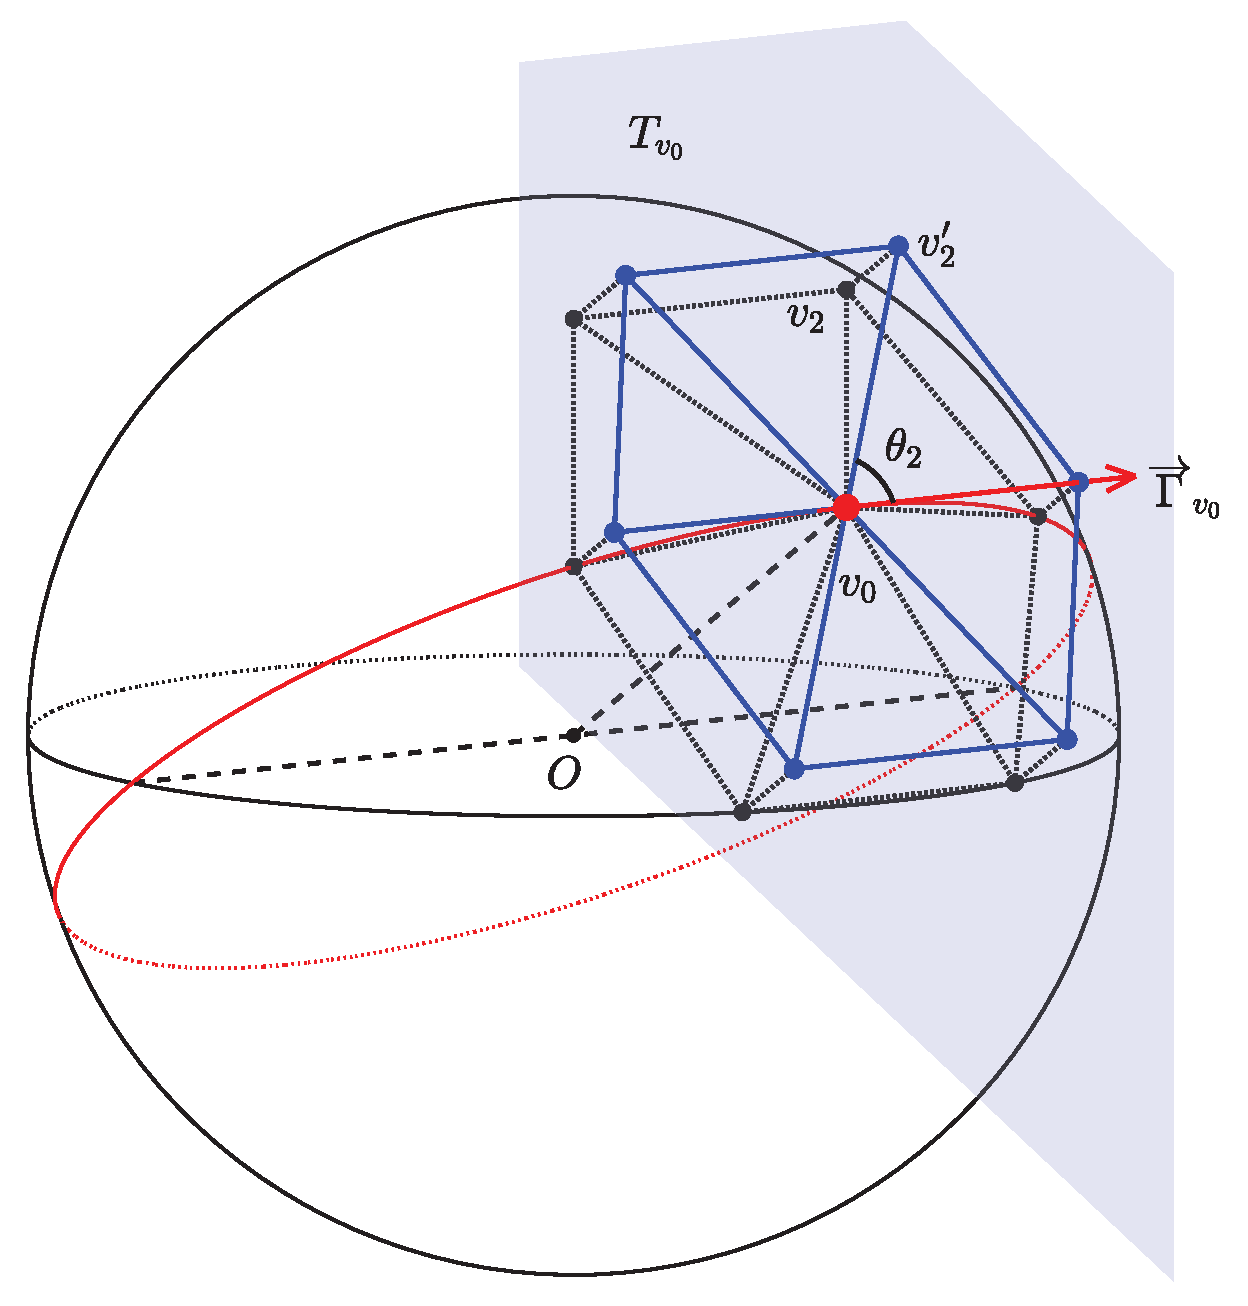
\includegraphics[width=0.5\linewidth]{figure/figure_1_ring_projection_on_tangent_plane.eps}
	\caption{1-ring卷积核邻域顺序的一致性定义。黑色的顶点$v_i$代表球面上的相邻顶点。蓝色的顶点$v_i'$是$v_i$在中心顶点$v_0$的切平面上的投影点。然后我们就可以根据$\theta_i$的大小得到邻点的顺序。}
	\label{fig:figure_1_ring_projection_on_tangent_plane}
\end{figure}
假设$v_0$为中心顶点,$v_i$为其1-ring卷积核中的相邻顶点,$i=1,2,\dots,5$(有5个邻点时)或$1,2,\dots,6$(有6个邻点时),$T_{v_0}$为球面在$v_0$处的切平面。我们定义$\vec{\Gamma}_{v_0}$为$v_0$处的切向量,沿球的大圆(great circle)指向$T_{v_0}$中的$x$轴。$\vec{\Gamma}_{v_0}$可由$\vec{n}_z\times \vec{v}_0$得到,其中$\vec{n}_z$是$XOY$平面的单位法向量。$\vec{v}_0$是由原点$O$到$v_0$的向量。对于极点的两个顶点,我们定义$\vec{\Gamma}_{v_0}=(1,0,0)$。接着再将顶点$v_i$投影到切平面$T_{v_0}$,得到投影顶点$v_i'\in T_{v_0}$。然后再计算每个相邻顶点与切平面内$x$轴之间的角度$\theta_i$:
\begin{equation}
\theta_i=\arccos{\frac{\vec{\Gamma}_{v_0} \cdot (\vec{v_i'}-\vec{v}_0)}{\Vert{\vec{\Gamma}_{v_0}}\Vert\Vert{\vec{v_i'}-\vec{v}_0}\Vert}}.
\end{equation}
通过对$\theta_i$进行排序,我们便可以将顺序1-6依次分配给相邻顶点,将0分配给中心顶点;对于只有5个邻接点的12个原始顶点,我们额外将6分配给中心顶点。

另外值得注意的是,一个完美地均匀分布着顶点的离散化球面并不存在\cite{lee2019spherephd}。本论文的实验表明,上述定义的1-ring卷积核具有所要求的$z$轴旋转不变性,并且不同顶点之间的方向与距离误差可以通过特征学习来克服\cite{lee2019spherephd,liu2018deep,zhao2019spherical_ipmi,jiang2018spherical}。在代码实现中,我们只使用上述方法计算一次相邻顶点的顺序,然后将其存储在内存中,后续计算时只需要通过矩阵索引即可实现快速的数据处理,这为本论文后续的方法提供了很高的计算效率。

\subsection{标准球面卷积操作}
根据1-ring卷积核的定义,在正二十面体离散化球面上的标准卷积(standard spherical convolution)操作可以很容易地定义,即1-ring卷积核与球面特征的加权过程,如图\ref{fig:fig_std_conv}所示。类似于2D/3D图像中的传统卷积操作,1-ring卷积核被用来在整个球面上对每个顶点进行卷积,以获得每个顶点的新的特征表达。2D/3D卷积中的步长(stride)概念在标准球面卷积操作中是不需要的,因为1-ring卷积核始终与每个顶点卷积,以获得每个顶点的新的特征向量。边缘填充(padding)在这里也不适用,因为球面卷积是在一个封闭的球面上进行的。球面卷积操作的作用是在同一个分辨率的离散化球面上,将特征图从一个维度转换到另一个维度,并进一步通过多层架构来学习和提取皮层属性的高级特征。

\begin{figure}[h]
	\centering
	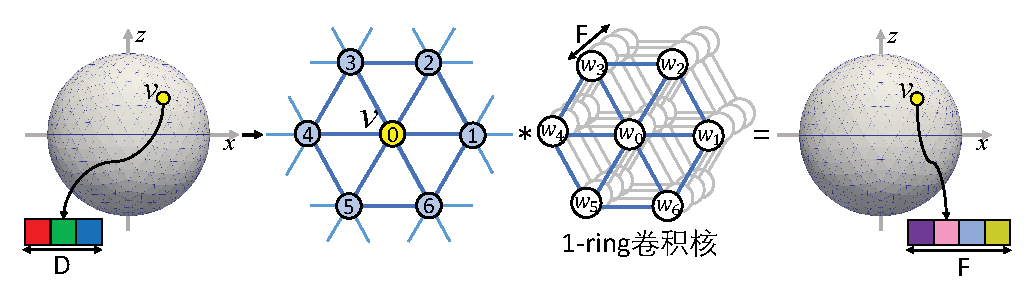
\includegraphics[width=\linewidth]{figure/figure_convolution.eps}
	\caption{基于1-ring卷积核的标准球面卷积操作。图示的卷积使用$F$个卷积核将带有$D$通道的输入特征图变成了带有$F$通道的输出特征图。}
	\label{fig:fig_std_conv}
\end{figure}

在具体实现中,对于一个具有$N$个顶点和$D$个通道特征图的球面来说,我们首先会提取每个顶点$v$和它的1-ring邻域的特征$I_v(7\times D)$,并将其变形(reshape)为属于该顶点的行向量$I_v'(1\times 7D)$。然后,对所有的$N$个顶点进行迭代,并将第一个维度堆叠(stack)起来,得到全节点的卷积矩阵$I(N\times 7D)$(参考MATLAB或其他深度学习工具箱中的“im2col”函数)。之后,在输出的通道数为$F$的情况下,通过将$I$与卷积层所要学习的卷积参数$W(7D\times F)$相乘,即可得到输出的新的特征图$O(N\times F)$。


\subsection{标准球面池化操作}
如图\ref{fig:fig_std_pooling}所示,球面上的标准池化操作(standard spherical pooling)与2D/3D图像上的也很相似。它主要用来增加网络的感受域(receptive field),减小特征表达的空间尺寸,以此减少网络中的参数数量和计算量。它与正二十面体的膨胀扩展过程相反,我们可以称之为正二十面体收缩过程。在第$i$个正二十面体分形体上,收缩过程将首先选择同样也在第($i$-1)个分形体上的中心顶点。这些顶点在收缩过程结束后仍将保留在球面上。然后把1-ring卷积核作为池化核应用到这些中心顶点上,再把第($i$-1)次分形球面上的边重新连接起来。便可以得到一个具有较少顶点的精细融合了上一级特征的池化球面。

\begin{figure}[h]
	\centering
	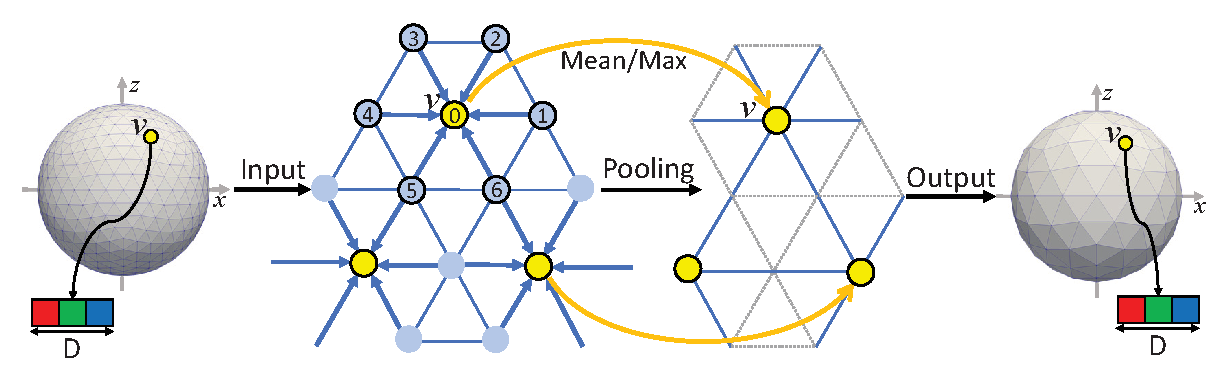
\includegraphics[width=\linewidth]{figure/figure_pooling_layer.eps}
	\caption{基于1-ring卷积核的标准球面池化操作。输入的第$i$次分形球面被池化到($i$-1)次分形球面上,同时特征图通道数$D$不变。}
	\label{fig:fig_std_pooling}
\end{figure}

同样在具体实现中,我们将从所有中心顶点的1-ring邻域中提取特征矩阵$I(N\times 7D)$。然后我们将其reshape为$I'(N\times D\times7)$。通过对$I'$的第3个维度取平均(平均池化)或最大值(最大池化),便可以得到池化后的特征图$O(N\times D)$。同时,顶点的数量从原始球面的$4N-6$减少为池化球面的$N$。

\begin{figure}[t]
	\centering
	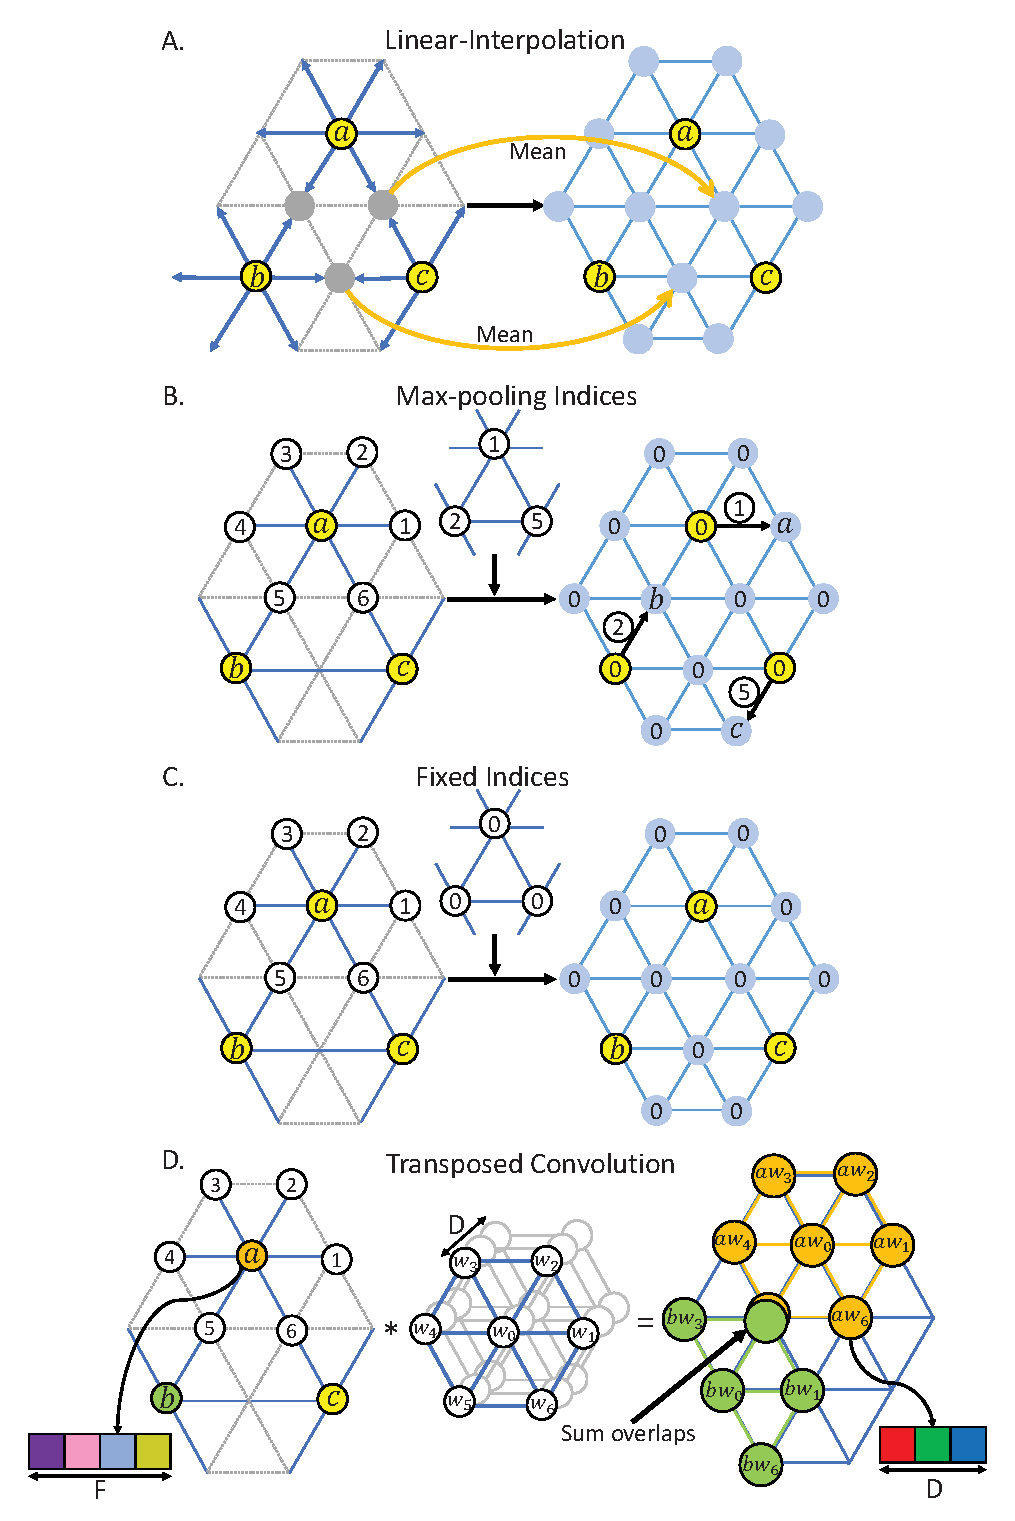
\includegraphics[width=0.8\linewidth]{figure/figure_upsampling_layer.eps}
	\caption{球面上的上采样方法说明。左边的输入特征图在($i$-1)次分形体上,右边的输出特征图在第$i$个分形体上,每个子图都显示了第$i$次分形体的特征图是如何从($i$-1)次分形体的池化特征图上采样得到的。}
	\label{fig:fig_upsampling}
\end{figure}

\subsection{球面上采样操作}
对正二十面体离散化球面数据进行上采样是从池化的低分辨率球面特征图中恢复原始的高分辨率球面的一个操作。因此,对于编码器解码器(encoder-decoder)结构\cite{badrinarayanan2017segnet}中的解码器的构建是至关重要的,尤其是对于逐个顶点的分类和预测任务。本小节同样基于1-ring卷积核,针对正二十面体离散化球面提出了几种流行的上采样方法。

\subsubsection{线性插值上采样(linear interpolation)}
球面上的线性插值遵循正二十面体的膨胀分形过程,它与平均池操作相反。对于每一个从三角形的边的中心生成的新的顶点,它的特征将由这条边的两个父顶点(parent vertices)的特征值进行插值得到,如图\ref{fig:fig_upsampling}A所示。

\subsubsection{最大值池化索引上采样(max-pooling indices)}
由SegNet\cite{badrinarayanan2017segnet}引入的最大池化索引上采样使用编码器存储的最大值池化索引,在相应的解码器中执行非线性上采样。我们将这种方法扩展到了球面上,如图\ref{fig:fig_upsampling}B所示。在编码器部分,首先最大值池化索引1、2和5分别被储存起来,它们是顶点a、b和c的1-ring邻域中的最大值。然后在相应的上采样层,分别用a、b、c的值来还原a的第1个邻点、b的第2个邻点和c的第5个邻点,其他顶点设为0。

\subsubsection{球面转置卷积(transposed convolution)}
转置卷积在U-Net中也被称为反卷积或上卷积(up-convolution)\cite{ronneberger2015u}。在2D/3D自然图像领域,转置卷积首先在所有原始像素上进行滑动窗口加权来恢复每个像素周围的像素,然后控制步长在恢复的重叠像素处进行求和。受这个思想的启发,我们将转置卷积也扩展到了球面上。对于一个球面的原始特征图$I$($N_i\times D)$,其中$N_i$表示第$i$个正二十面体分形体上的顶点数,$D$表示特征数,还有它的池化的特征图$O$($N_{i-1}\times F)$。我们可以通过首先使用1-ring卷积核对池化的$O$上的每个顶点做转置卷积,然后对重叠的顶点进行求和来还原$I$,如图\ref{fig:fig_upsampling}D所示。

\subsection{球面U-Net的构建}\label{sec:球面U-Net的构建}
基于上述我们定义的球面卷积、池化和转置卷积操作,我们搭建了球面U-Net结构,如图\ref{fig:fig_unet}所示。它有一个编码器和一个解码器,分别有5个不同的分辨率级别,用$i$来表示,即$i=1,2,\dots,5$。与标准的U-Net\cite{ronneberger2015u}不同的是,我们用1-ring卷积核代替了所有的3$\times$3卷积,用球面转置卷积代替了2$\times$2的标准转置卷积,用球面最大/平均值池代替了2$\times$2最大值池化。另外在此基础上,我们还在每个卷积层的ReLU(Rectified Linear Unit)激活函数前,增加了一个批量归一化层(Batch Normalization, BN)。在最后一层,1$\times$1的卷积被vertex-wise的加权平均所取代,用来将倒数第二层的$C_1$通道的特征向量映射到最后一层所需的$C_{out}$通道。另外,在球面U-Net中,特征通道数在每个球面池化层后翻倍,并在每个转置卷积层后减半,使得$C_{i+1}=C_i\times 2$,$N_{i+1}=(N_i+6)/4$。值得注意的是,我们不需要在原始U-Net\cite{ronneberger2015u}中使用的平铺策略来实现无缝的输出图,因为球面U-Net中所有的数据都在一个封闭的球面上。

\begin{figure}[t]
	\centering
	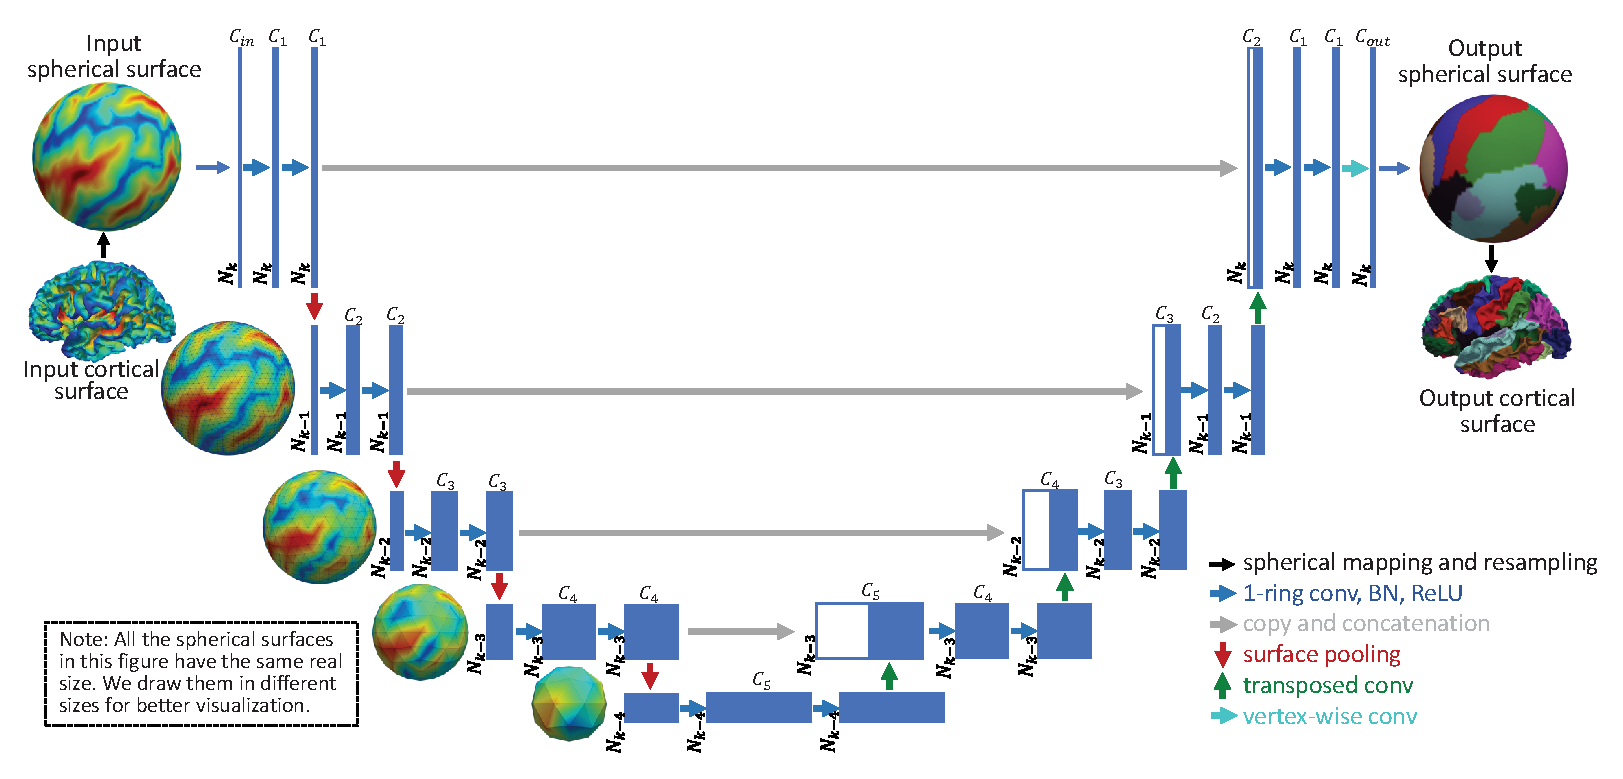
\includegraphics[width=\linewidth]{figure/figure_unet.eps}
	\caption{球面U-Net结构。蓝色方框代表球面空间上的特征图。特征的数量$C_i$标在框的上方。顶点数量$N_i$标在方框的左下角。$N_{i+1}=(N_i+6)/4$,$C_{i+1}=C_i\times 2$。$N_1$一般是10242、40962或163842,$C_1$通常设置为64。在我们的应用中,输出的球面是皮层分区图或预测的皮层属性图。}
	\label{fig:fig_unet}
\end{figure}

\section{球面可变形U-Net}
上述使用1-ring卷积核构建的球面U-Net本质上依然局限于模拟比较大的固定变换\cite{dai2017deformable}。然而由于皮层褶皱的形状和大小变化很大,开发应用于皮层的深度学习卷积核的另一个挑战就是如何模拟并自动调节针对不同皮层结构的不同变换。这个缺陷来自于1-ring卷积核的固定设计,因为1-ring卷积核在每一个操作中,例如球面卷积、池化,都使用固定位置的邻点对输入特征图进行采样。这样一来,同一层中所有顶点的感受域是相同的,然而深层网络的每一层都需要在空间位置上编码高级语义信息,由此来表达不同形状和大小的图像结构,固定的感受域在这种情况下明显不太适合搭建深层神经网络。因此传统的CNN在几何变换建模这一方面存在固有的缺陷。为了解决这个问题,Deformable Convolutional Network(DCN)\cite{dai2017deformable}提出在卷积和池化层中使用额外的偏移量来变换空间采样位置,并从目标任务中学习任务特定的偏移量。因此DCN可以自适应地学习各种几何变换。另外一些相关工作在几何变换建模方面也使用了这一概念,但只基于一些先验知识做了特定变换,如尺度\cite{xu2014scale}和旋转\cite{worrall2017harmonic}。空间变换网络(Spatial Transformer Networks, STN)\cite{jaderberg2015spatial}是第一个直接从数据中学习几何变换的方法。它的目的是学习一个全局的变换,如affine变换,然后用来对特征图进行形变或扭曲。而DCN更注重局部的、可变形的变换,并且没有特征形变步骤,因此更容易集成到流行的CNN架构中。当可变形卷积中的偏移量固定在一些特定的稀疏位置时,可变形卷积就退化成了空洞卷积\cite{chen2017rethinking},即将原卷积核的权值保持在固定的稀疏位置。这是DCN的一种特殊情况。因此,DCN是一种比较通用的CNN模型,可以灵活地调整感受域的大小,大大增强CNN的变形建模能力。同时,它还具有轻量级和易于训练的特点,对于需要密集预测的复杂视觉任务具有非常有效的作用\cite{dai2017deformable}。

因此,受到欧几里得空间中的可变形卷积网络DCN\cite{dai2017deformable}的启发,本论文学习了它的变形增强卷积层和池化层的概念,提出将1-ring卷积核进一步发展为球面可变形1-ring卷积核(deformable 1-ring filter),开发了球面可变形卷积和球面可变形池化操作,并进一步提出将DCN模型扩展到球面,以对皮层表面数据的各种复杂未知的变换进行建模。具体来讲,它在常规的1-ring卷积核采样位置上增加了球面偏移量,从而使1-ring卷积核可以自由地变形,用于自适应地定位不同尺寸和形状的皮层结构。另外它们都是轻量级的,可以很容易地取代它们之前的标准球面操作,从而方便搭建新的球面可变形U-Net(Spherical Deformable U-Net, SDU-Net)。

\subsection{球面变形卷积与池化操作}
如图\ref{fig:fig_deform_conv}和图\ref{fig:fig_deform_pool}所示,球面偏移量首先是通过在相同的输入特征图上应用标准
\begin{figure}[h]
	\centering
	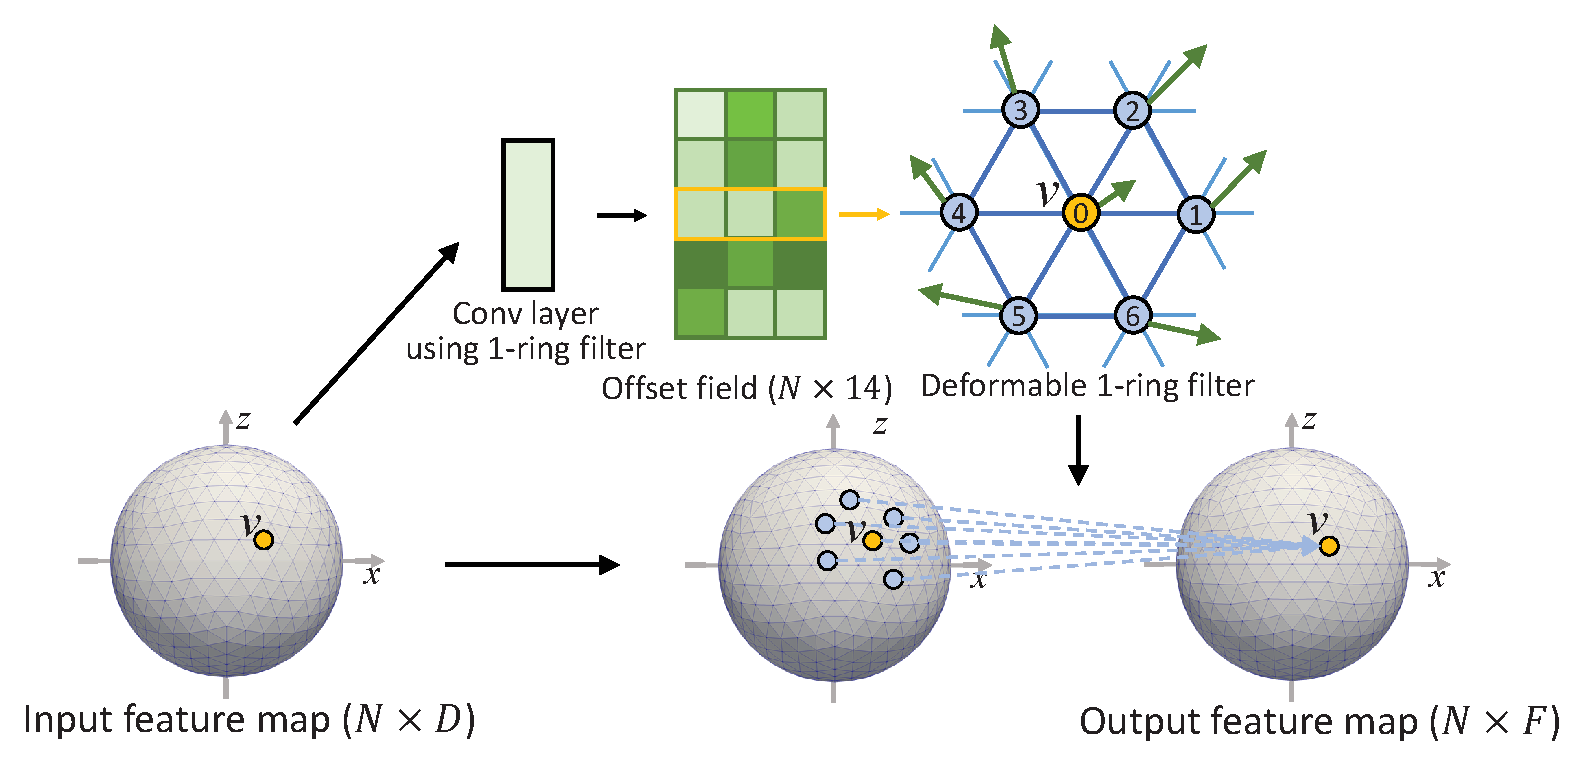
\includegraphics[width=0.85\linewidth]{figure/spheircal_deform_conv.eps}
	\caption{球形变形卷积操作。}
	\label{fig:fig_deform_conv}
\end{figure}
的球面卷积层得到的。输出偏移场由大小为$N\times 14$的切向量表示。每个顶点的切平面是在该顶点处定义的,这意味着每个顶点都有一个不同的切平面。通道数14对应每个顶点$v_n$的1-ring卷积核的7个邻点${\{v_{n,i}\}}_{i=1}^7$($i$代表第$i$个邻点)的切向量${\{\overrightarrow{u_{n,i}}\}}_{i=1}^7$。那么$E_{n,i}\overrightarrow{u_{n,i}}$则会将切向量从切平面空间映射到三维空间,其中$E_{n,i}=[\overrightarrow{e_{n,i}^1},\overrightarrow{e_{n,i}^2}]$是$v_{n,i}$处切平面空间上的$3\times 2$的正交基。那么在一个单位球体上,变形后的采样位置$\{v_{n,i}'\}_{i=1}^7$就可以被定义为:
\begin{equation}\label{equ:equ2-2}
v_{n,i}'=\frac{v_{n,i}+E_{n,i}\overrightarrow{u_{n,i}}}{\Vert v_{n,i}+E_{n,i}\overrightarrow{u_{n,i}}\Vert},
\end{equation}
通过这种方式,常规的1-ring卷积核被变形了并增加了额外的球面偏移量$\overrightarrow{u_{n,i}}$,从而实现了对不同位置的感受域的自适应学习。然后我们将变形后的1-ring卷积核的采样位置的特征值与1-ring卷积核进行加权,就可实现球面变形卷积,或球面变形池化操作。值得注意的是,变形采样位置最终会被归一化到球面上,因此它在切平面上的范围并不是无限大的,而是在$(-\pi/2,+\pi/2)$的球形范围内。尽管如此,在实践中我们发现变形大小仍然在一个很小的范围内,这个范围即使对于皮层分区图上比较大的ROI而言,也是一个合理的变形大小。在这种情况下,切平面和球面上的变形点非常接近。它们之间简单而近似相等的关系(公式\ref{equ:equ2-2})可以很容易地被网络学习到,从而找到球体上实际的最佳变形采样位置。由于$\overrightarrow{u_{n,i}}$通常是小数,所以$v_{n,i}'$处的特征值是通过重心插值法\cite{yeo2009spherical}计算出来的。最后,由于所有的运算都是可导的,网络中的梯度便可以有效地反向传播用来训练卷积核中的权值,这些权值随后就可以用于同时生成输出特征图和偏移量。

\begin{figure}[t]
	\centering
	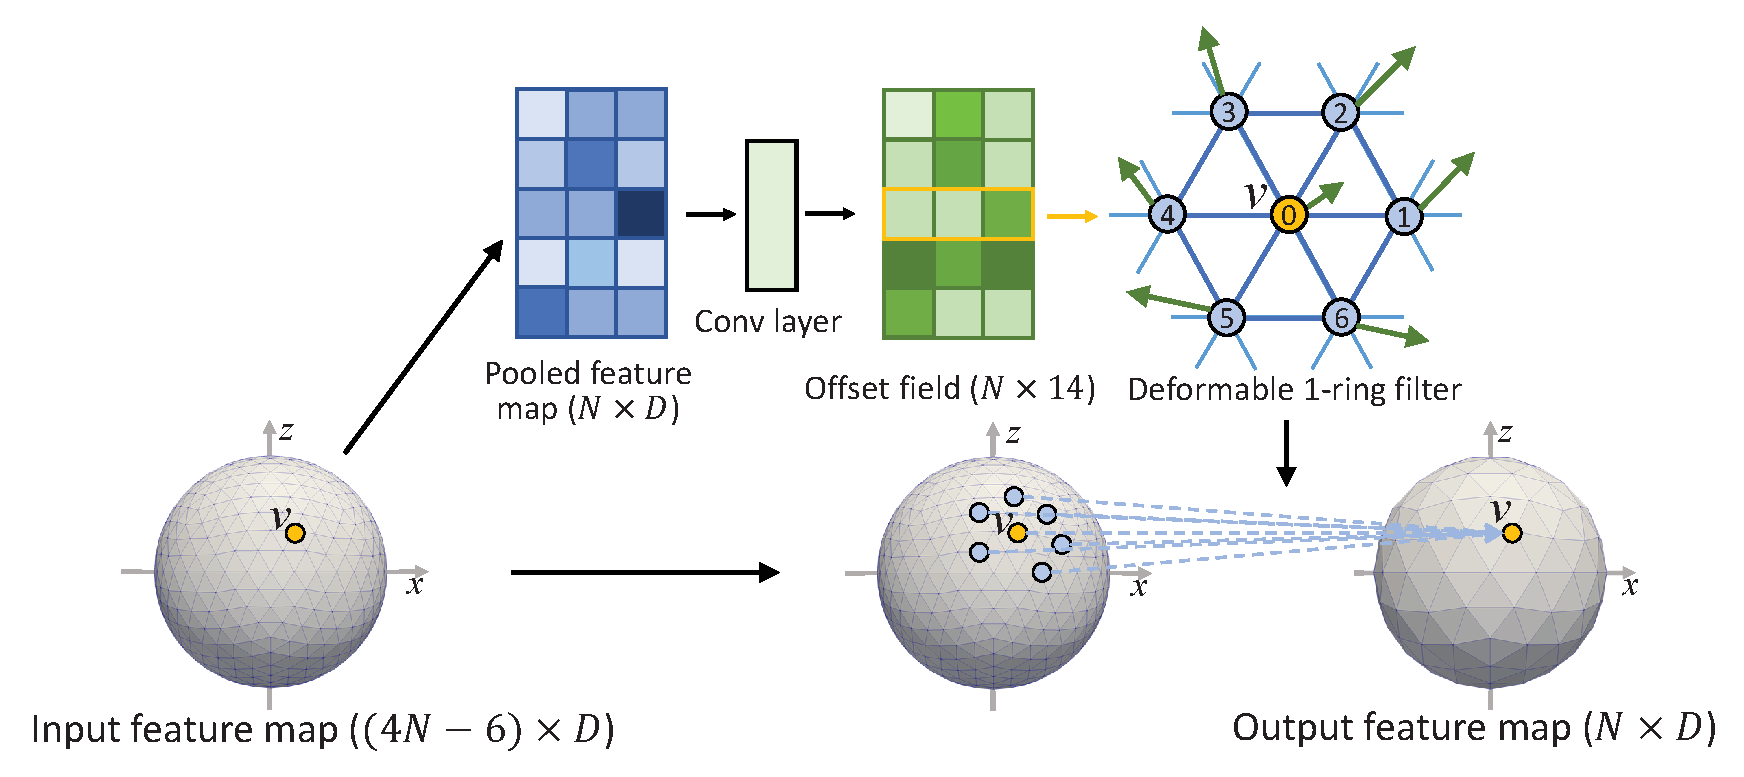
\includegraphics[width=0.85\linewidth]{figure/spheircal_deform_pool.eps}
	\caption{球形变形池化操作。}
	\label{fig:fig_deform_pool}
\end{figure}

\subsection{球面可变形U-Net的构建}
在\ref{sec:球面U-Net的构建}球面U-Net的基础上,为了增强球面U-Net的几何变换建模能力,本论文把变形卷积和池化操作整合进了球面U-Net并搭建了SDU-Net,用来自适应地模拟各种不同尺寸和形状的皮层结构以满足不同皮层表面应用的需求。由于这两种可变形运算的输入和输出都与标准版本相同,因此它们可以很容易地替代球面U-Net中的对应的运算,同时增加的运算量也不是很大,这将在后面的实验部分证明。如图\ref{fig:fig_sdunet}所示,SDU-Net的基本结构与球面U-Net一致。编码器由8个球面卷积层和3个球面池层组成。球面可变形操作应用于前4个卷积层和所有池化层。我们对不同的层数是否应用可变性操作也进行了对比实验,发现如图\ref{fig:fig_sdunet}这种配置对于不同的任务来说是一种最好的结果。然后,由球面转置卷积和卷积层组成的解码器从编码器提取的特征图中生成最终的结果。SDU-Net的通道数与分辨率层数也与它的标准版本的球面U-Net一致。

\begin{figure}[t]
	\centering
	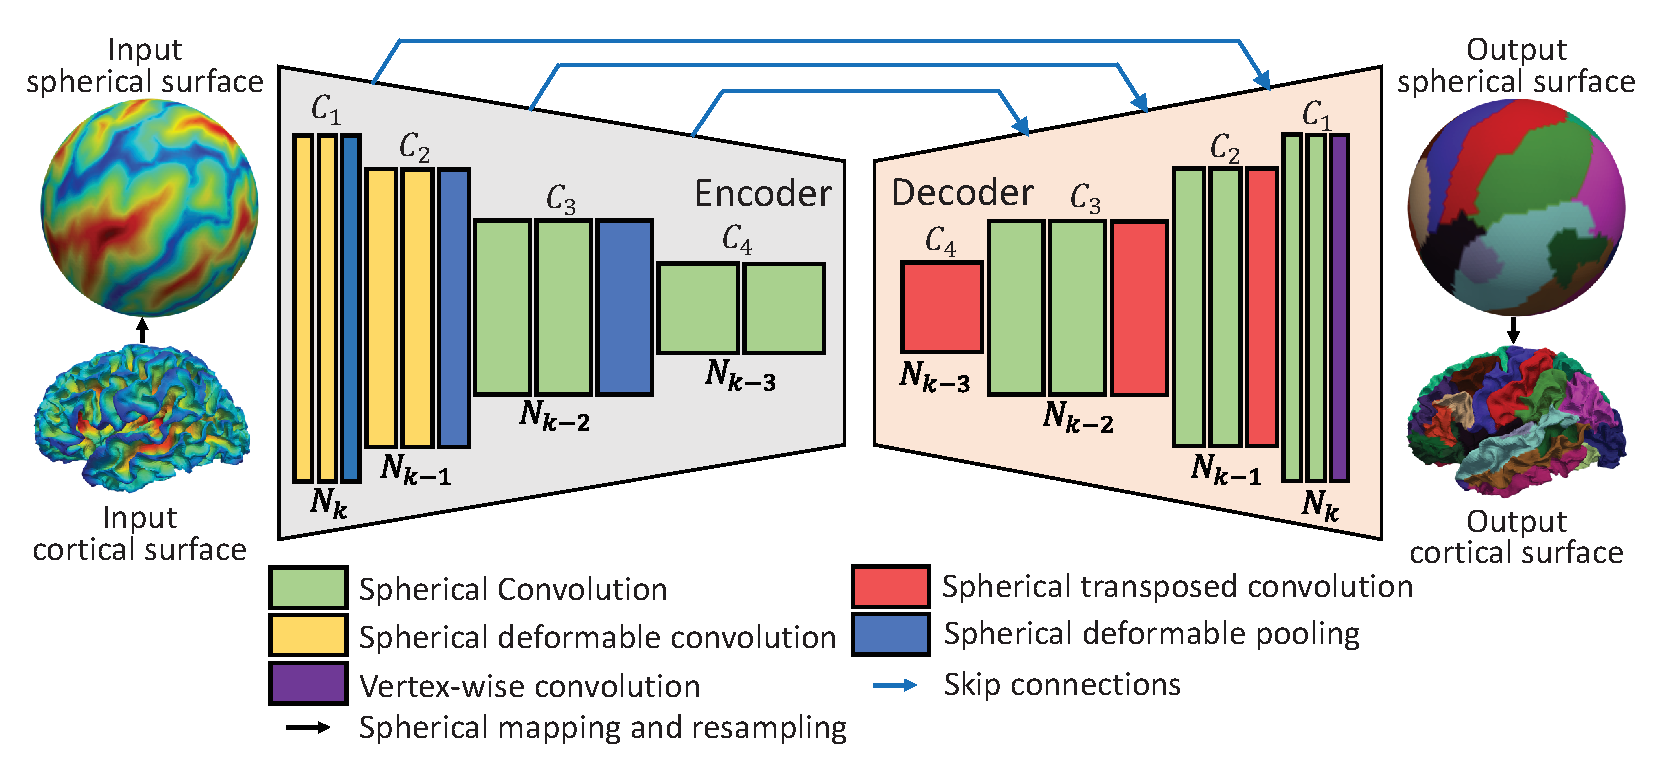
\includegraphics[width=0.9\linewidth]{figure/spheircal_deform_cnn}
	\caption{球面可变形U-Net网络结构。每次操作后得到的特征数$C_i$标记在了方框上方。顶点的数量$N_i$标记在了方框的下方。$N_{i+1}=4N_i-6$, $C_{i+1}=C_i\times 2$。输入顶点数$N_k$中的$k$表示输入球面在第$k$个二十面体分形体离散球面上。通常情况下,我们使用正二十面体的第7或第8个分形体,分别有40962和163842个顶点,$C_1$一般设为64。}
	\label{fig:fig_sdunet}
\end{figure}



%%%%%%%%%%%%%%%%%%%%%%%%%%%%%%%%%%%%%%%%%%%%%%%%%%%%%%%%%%%%%%%%%%%%%%%%%%%%%%%%%%%
%% 第二章 基于球面U-Net的皮层分区与属性预测 实验部分
%%%%%%%%%%%%%%%%%%%%%%%%%%%%%%%%%%%%%%%%%%%%%%%%%%%%%%%%%%%%%%%%%%%%%%%%%%%%%%%%%%%


\section{大脑皮层分区实验}\label{sec:大脑皮层分区实验}
\subsection{实验设计}\label{sec:大脑皮层分区实验实验设计}
将大脑皮层表面自动准确地分成结构和功能上有意义的区域,在人类大脑皮层的分析中具有根本性的重要意义\cite{meng2015automatic}。在基于区域或网络的大脑研究中,它对于区域定位和个体之间的比较至关重要。传统的基于配准的方法\cite{meng2015automatic,yeo2009spherical,fischl2004automatically}需要设计特定的人工特征来将皮层形状映射到分区标签(ROI label)上,这不仅耗时还需要专家经验的介入。由于对不同的神经解剖专家的依赖性强,因此很容易出现经验不一致错误。在本论文中,我们将这个分区问题看作是一个语义分类问题来解决,使用我们的基于深度学习的球面U-Net及其变种来对整个皮层表面进行分区,即对每个顶点进行密集分类,给每个顶点都分配一个分区的标签。

本实验采用了NAMIC成人数据集\cite{meng2015automatic}和一个在北卡罗莱纳大学教堂山分校(University of North Carolina at Chapel Hill, UNC)采集的婴儿数据集。NAMIC数据集包含了39个成人大脑MR图像。UNC婴儿数据集包含了90个婴儿大脑MRI数据。NAMIC数据集中的所有皮层表面均使用FreeSurfer\cite{fischl2012freesurfer}pipeline进行了重建。婴儿大脑皮层表面使用了婴儿专用的MRI数据处理pipeline\cite{li2015construction,2014measuring}(iBEAT V2.0 Cloud, http://www.ibeat.cloud/)进行重建。我们在这篇论文中只关注大脑的左半球,因为右半球是类似的。重建后的左半球皮层表面的每个顶点都含有3个形态学属性值,即平均曲率(mean curvature, curv)、平均凸度(average convexity, sulc)和脑沟深度(sulcal depth)。其中,curv是精细度量皮层折叠的评价指标;sulc是粗略度量皮层折叠的评价指标;sulcal depth是结合了粗略视图和精细视图的皮层折叠评价指标。这些形状度量指标反映了皮层表面的局部几何属性,这对于皮层表面的分区是十分有用的\cite{desikan2006automated}。随后根据FreeSurfer定义的皮层分区\cite{desikan2006automated},每个皮层表面都由神经解剖学家依据大脑沟回形态手动分成35个区域。最后所有的大脑皮层都被映射到球面空间,然后重采样到正二十面体第7次分形体离散化球面上(40962个顶点)。

为了更好地展现模型的泛化能力,我们使用60\%的数据进行训练,15\%的数据进行验证,25\%的数据进行测试。我们首先在15\%的验证集和60\%的训练集之间进行了5次的交叉验证。然后,基于5次交叉验证的结果我们选出每个模型最好的超参数,并基于最好的超参数用训练集重新训练好每一个模型,然后在单独保留的测试集上测试每一个模型的表现。在训练时,我们使用了交叉熵损失函数(cross-entropy loss)和Adam优化算法\cite{kingma2014adam}来更新网络的可训练参数,并且把学习率减小5倍一旦训练Dice停滞2个回合(epoch)。我们通过随机绕$z$轴旋转球面50次来进行数据增强(data augmentation)。为了进行定量评估,正如\cite{yeo2009spherical}所做的一样,我们计算了所有测试数据的平均Dice\cite{dice1945measures}指标。

\subsection{基准模型}
实验使用了如图\ref{fig:fig_unet}所示的球面U-Net结构展现了本论文提出的球面神经网络的优越性能,并用图\ref{fig:fig_sdunet}所示的SDU-Net结构研究了可变性卷积和池化的作用。我们将$C_{in}$统一设置为3,对应3个形状属性,$C_{out}$设置为35,对应35个ROI标签,$k$设置为7,所以$N_k=40,962$,$C_1$设置为32。为了研究网络参数的大小和过拟合的影响,我们将图\ref{fig:fig_unet}所示的球面U-Net也称为球面U-Net23,将拥有3个分辨率级别18个卷积层的球面U-Net称为球面U-Net18。

为了更好地验证球面可变形操作的有效性,我们将球面可变形操作与其他最先进的语义分割CNN架构进行了结合。注意到这些架构一般由两个网络组成,一个是学习输入图像高级特征表达的编码器,另一个是针对不同任务从编码后的特征图中生成结果的解码器,我们便使用了与SDU-Net中相同的编码器以及其他两个先进的解码器结构来做比较实验,即SegNet\cite{badrinarayanan2017segnet}和FCN\cite{long2015fully}。SegNet是一个优秀的语义分割方法,球面SegNet(Spherical SegNet)与SDU-Net在两个方面有所不同:(1)球面SegNet中没有复制和跳转连接;(2)对于上采样操作,球面SegNet使用线性插值。FCN是另一种流行的分割网络。我们使用了传统的FCN-8s\cite{long2015fully}作为基础结构,因为它是能将高层信息和低层信息结合起来的最佳FCN变体,再将相应操作拓展到球面上后便搭建了球面FCN-8s架构(Spherical FCN-8s)。球面FCN-8s会在每个池化层之后,将不同分辨率的特征图进行结合,最后利用转置卷积层将结合后的特征图映射到所需的输出通道。

\begin{table}[h]
		\caption{\label{tab:婴儿数据集分区结果}在网络的编码器部分使用不一样的可变形卷积或池化层的婴儿脑皮层分区结果。}
		\centering
		\zihao{5}
		\begin{tabularx}{\linewidth}{l X<{\centering} X<{\centering} X<{\centering} X<{\centering}}
			\Xhline{2\arrayrulewidth}
			\makecell{球面变形操作的使用情况\\ (\# layers)}& 球面U-Net23      & 球面U-Net18     &  球面SegNet & 球面FCN-8s   \\
			\hline
			无变形操作的基准模型                    &  92.67±1.60            &	92.28±1.70       &  89.49±3.52       	 &		91.75±1.55 \\   
			
			2 deformable conv layers (1-2)           &	93.09±1.57           &	92.78±1.72		 &  89.72±2.60           &	92.10±1.50  \\
			4 deformable conv layers (1-4)           & 	\textit{93.15±1.40}	& \textit{92.85±1.57}	& \textit{90.04±2.19}			&92.15±1.59  \\
			6 deformable conv layers (1-6)           & 	92.97±1.59	&		92.76±1.70	&		90.01±2.40	&		\textit{92.16±1.51} \\
			6 deformable conv layers (3-8) 	         &	93.05±1.58	&		92.75±1.87	&		90.01±2.67		&	92.10±1.60 \\
			
			Spherical deformable pooling            &  	92.98±1.56	&	92.61±1.67	&		89.95±2.56	&		92.06±1.62\\
			
			\makecell{Spherical deformable pooling+\\4 deformable conv layers (1-4)} &	\textbf{93.20±1.40} &	\textbf{93.07±1.51}	& \textbf{90.06±2.11}	&  \textbf{92.41±1.51}	 \\
			\Xhline{2\arrayrulewidth} 
		\end{tabularx}
\end{table}

\subsection{实验结果}
\textbf{球面变形卷积。}表\ref{tab:婴儿数据集分区结果}展示了球面可变形卷积在不同结构下的不同使用效果。当使用更多的可变形卷积层时,Dice指标明显稳步提高。当球面FCN-8s的前6个卷积层为可变形卷积层,其他网络的前4个卷积层为可变形卷积层时,便可以得到最优结果。因此,在接下来的实验中,我们将在特征提取网络的前4个卷积层中使用可变形卷积层。为了更好地理解球面可变形卷积的原理,图\ref{fig:receptivefield_sampling_points}
\begin{figure}[h]
	\centering
	\includegraphics[width=0.9\linewidth]{figure/receptivefield.eps}
	\caption{经过三个连续的卷积层,在两个不同的激活点(两个绿点分别在第一行的一个小的ROI和第二行的一个比较大的ROI上)上的1-ring卷积核的采样位置与皮层ROI分区图(即固定的3-ring的感受域),可变形的1-ring卷积核的采样位置与皮层ROI分区图,可变形的1-ring卷积核的采样位置与sulc特征图,可变形的1-ring卷积核的采样位置与curv图。可以看到对于不同的结构,感受域是如何自适应转换的。}
	\label{fig:receptivefield_sampling_points}
\end{figure}
中展示了使用普通的1-ring卷积核和可变形的1-ring卷积核在连续3个卷积层后的采样点位置。由此我们可以观察到,在连续的可变形卷积层中,学习到的球面偏移量对不同的皮层结构具有很强的自适应能力。

\textbf{球面变形池化。}如表\ref{tab:婴儿数据集分区结果}所示,与基准模型相比,单独使用球面可变形池化操作已经改善了基准模型的Dice指标。当同时使用球面可变形卷积和池化时,可以获得更加显著的改进,并得到所有网络的最佳变种模型。

\textbf{模型复杂度和运行时间。}表\ref{tab:模型复杂度和运行时间结果}
\begin{table}[h]
		\caption{\label{tab:模型复杂度和运行时间结果}球面可变形网络与普通网络的模型复杂度和运行时间比较。}
		\centering
		\zihao{5}
		\begin{tabularx}{0.85\linewidth}{c X<{\centering} X<{\centering}}
			\Xhline{2\arrayrulewidth}
			网络结构 & 参数数量 (百万)           & 运行时间 (毫秒)         \\
			\hline
			Spherical U-Net23                & 26.86      &    20.3 \\
			SDU-Net23    &  	26.89           		&   51.9   \\   
			Spherical U-Net18               & 1.67                  	&	4.1	 \\
			SDU-Net18   &	1.68	                &	13.2	  \\
			Spherical SegNet                 & 	1.37                    &			3.5 \\
			Spherical Deformable SegNet    &			1.39            &  	 12.2	 \\
			Spherical FCN-8s                 &  		\textbf{1.01}                &	\textbf{3.0}	 \\
			Spherical Deformable FCN-8s   & 	1.02                    &11.5  \\
			\Xhline{2\arrayrulewidth} 
		\end{tabularx}
\end{table}
显示了球面可变形网络及其普通版本在NVIDIA Geforce GTX2080 Ti GPU上的模型复杂度和运行时间。我们可以看到,球面可变形操作只在模型参数和计算量上增加了一点点的负担。这说明性能的提升是来自于模型的几何变换建模能力,而不是单纯依赖增加模型参数。相反,球面U-Net23在增加了更多参数和运行时间的情况下也只取得了稍微好一点点的结果。因此,考虑到速度和实用性,我们把球面可变形U-Net18当作默认的SDU-Net模型,并在下面的实验中将它与其他流行的皮层分区方法进行比较。

\textbf{上采样方法。}除了编码器部分的可变形卷积和池化外,实验还对比研究了SDU-Net的解码器部分的上采样方法,比如在\cite{jiang2018spherical,parvathaneni2019cortical}中使用的Fixed Indices,并将结果展示在了表\ref{tab:上采样方法比较}中。
\begin{table}[h]
		\caption{多种上采样方法在婴儿脑皮层表面分区任务上的对比结果}
		\label{tab:上采样方法比较}
		\centering
		\zihao{5}
		\begin{tabularx}{0.75\linewidth}{X<{\centering}  X<{\centering}}
			\Xhline{2\arrayrulewidth}
			网络结构  & Dice (\%)        \\
			\hline		  
			SDU-Net-Linear Interpolation     &     92.91±1.52   \\
			SDU-Net-Max-pooling Indices      &     86.69±3.74   \\
			SDU-Net-Fixed Indices            &     92.85±1.98    \\
			SDU-Net-Transposed Convolution   &	   \textbf{93.07±1.51}  \\
			\Xhline{2\arrayrulewidth}					 
		\end{tabularx}
\end{table}
表中的结果验证了球面转置卷积的优越性,这得益于它不仅可以上采样皮层球面,还可以同时训练其中的可学习上采样卷积核的参数,从而有效地解决了在球面上上采样数据的问题。但同时我们也注意到,与其他上采样方法相比,转置卷积带来的效果提升并不是很明显。一个可能的原因是对于其他3种上采样方法,我们在它们之后都增加了一个标准的1-ring球面卷积层,用于匹配通道数,这增加了他们的参数数量同时也提高了它们的学习能力。图\ref{fig:par_results_roiwise}展示了使用不同方法得到的每个ROI的平均Dice指标的直观比较,可以看到SDU-Net几乎在所有ROI中都获得了最高的Dice值。图\ref{fig:par_results_35}展示了使用不同方法得到的一个婴儿大脑的皮层分区结果,可以看到SDU-Net得到的分区结果与人工标记的金标准非常一致,没有什么孤立的噪声点。
\begin{figure}[t]
	\centering
	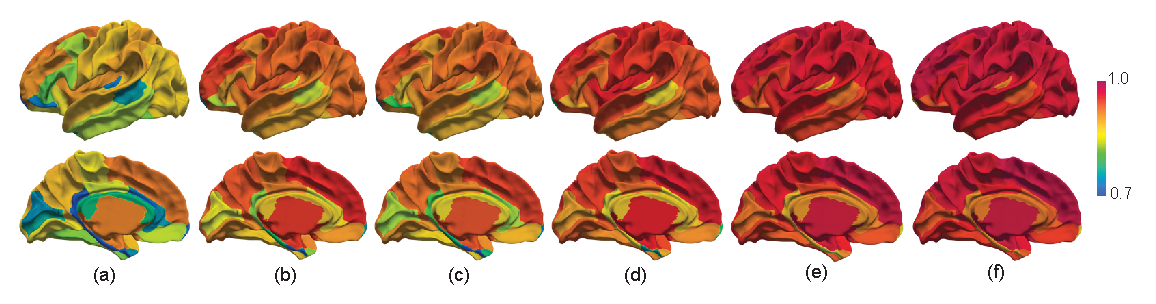
\includegraphics[width=\linewidth]{figure/figure_roi_result.eps}
	\caption{ROI-wise皮层分区Dice结果。图中每个ROI显示的值即为该ROI的平均Dice值。从左到右的方法依次是:(a) SegNet-Max Indices;(b) SegNet-Fixed Indices;(c) SegNet-Linear Interpolation;(d) Spherical FCN-8s;(e) 球面U-Net23;(f) SDU-Net。}
	\label{fig:par_results_roiwise}
\end{figure}

\begin{figure}[h]
	\centering
	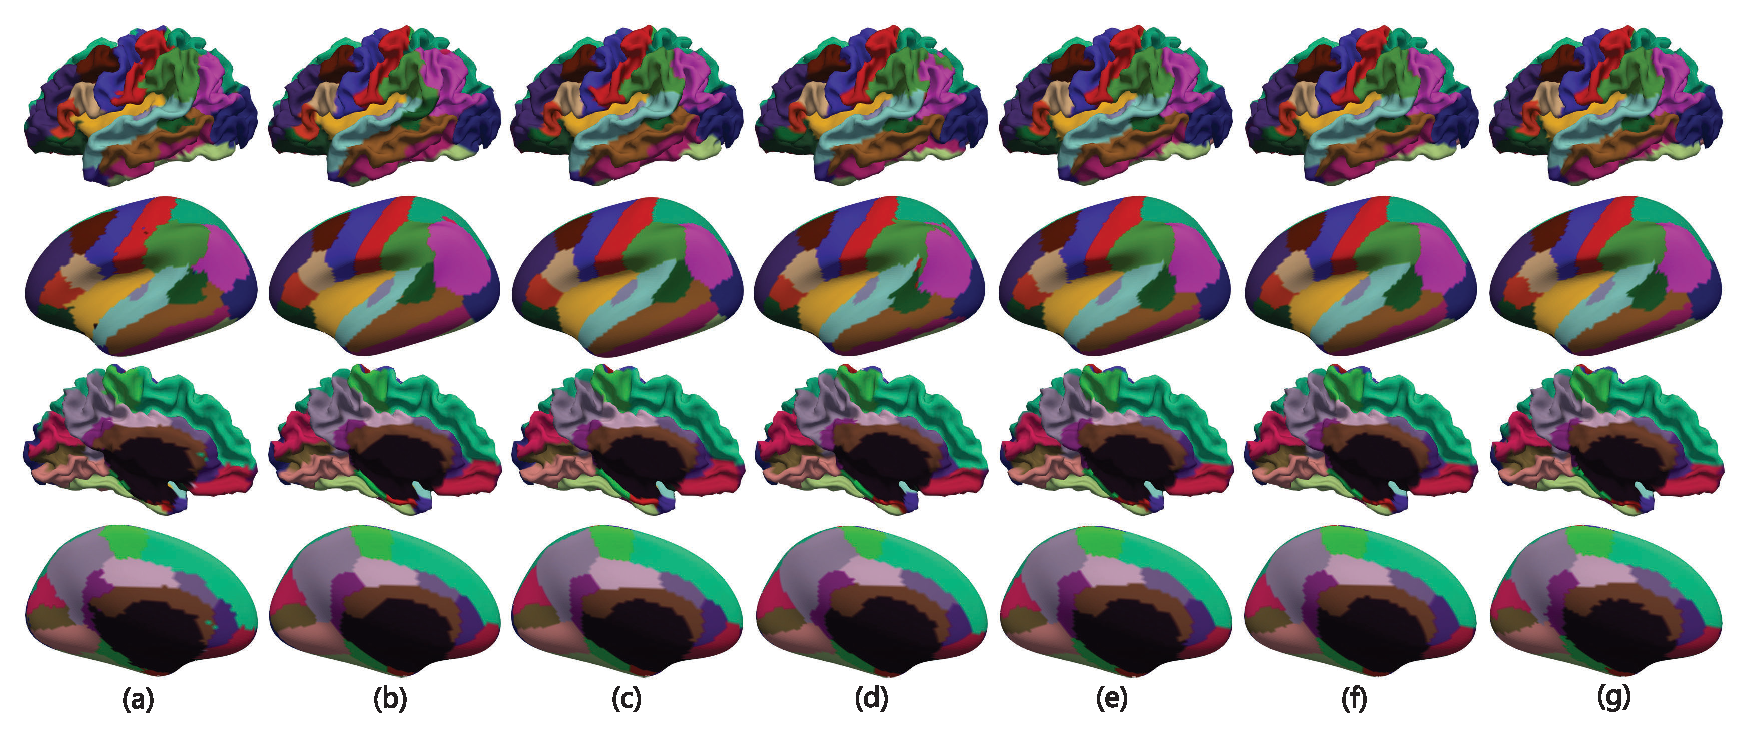
\includegraphics[width=\linewidth]{figure/figure_parcellation_result.eps}
	\caption{在一个随机选择的婴儿大脑皮层上的分区结果。(a) SegNet-Max Indices;(b) SegNet-Fixed Indices;(c) SegNet-Linear Interpolation;(d) Spherical FCN-8s;(e) 球面U-Net23;(f) SDU-Net;(g) 金标准。}
	\label{fig:par_results_35}
\end{figure}


\textbf{与其他球面CNN的比较。}因为利用等角投影(Equirectangular projection, ERP)对球面进行离散化的方法\cite{s2018spherical,hu2017deep,esteves2018learning}显然不适合皮层表面的应用\cite{zhao2019spherical_ipmi,zhao2019spherical_isbi,lee2019spherephd},所以我们只比较了目前比较流行的球面CNN\cite{wu2018registration,jiang2018spherical,seong2018geometric}。这些CNN都是直接在正二十面体离散化球面上进行卷积的。如表\ref{tab:与其他球面CNNs的比较}所示,本论文提出的SDU-Net的表现优于在切平面使用裁切补丁的分类方法\cite{wu2018registration}和使用全局差分滤波器的方法\cite{jiang2018spherical}。这表明我们的方法成功地从皮层表面的邻域中学习了多层的高级特征表示,而这正是以往工作\cite{wu2018registration,jiang2018spherical}所缺乏的。同时这些结果也再一次印证了SDU-Net比它的标准版本的球面U-Net\cite{zhao2019spherical_ipmi}的结果要好。最后,与图\ref{fig:fig_filters}中的2-ring卷积核和切平面空间中的矩形5$\times$5卷积核做了比较,可以看出虽然他们在特征学习方面也很有效,但本论文提出的1-ring卷积核在内存存储方面要小得多,而且在模型大小方面也更轻量。
\begin{table}[t]
		\caption{本论文提出的方法与其他球面CNN在婴儿脑皮层分区的结果比较。}
		\label{tab:与其他球面CNNs的比较}
		\centering
		\zihao{5}
		\begin{tabularx}{0.8\linewidth}{c  X<{\centering}}
			\Xhline{2\arrayrulewidth}
			球面CNN & Dice (\%)        \\
			\hline
			Wu et al. \cite{wu2018registration}										&   87.06\\
			Jiang et al. \cite{jiang2018spherical, parvathaneni2019cortical}		& 	75.15±3.09		\\
			球面U-Net18-矩形卷积核\cite{seong2018geometric,zhao2018distortion,tateno2018distortion}	& 	92.24±1.98\\
			球面U-Net18-1-ring卷积核 			&   92.28±1.70\\
			球面U-Net18-2-ring卷积核 				    &   92.28±2.03\\
			SDU-Net  											&	\textbf{93.07±1.51} \\
			\Xhline{2\arrayrulewidth} 
		\end{tabularx}
\end{table}

\textbf{与其他大脑皮层分区方法的比较。}由于以前的大脑皮层分区方法\cite{yeo2009spherical,meng2015automatic,desikan2006automated}都是在配准后再训练分类器来对皮层表面的特征进行模式识别。于是我们先使用了Spherical Demons算法\cite{yeo2009spherical}对NAMIC数据集中的所有球形皮层表面进行了基于群体的配准,并分别在配准前后对球面进行了重采样。为了直接与他们的结果进行比较,本实验采用了不同于前几个对比实验的4折交叉验证策略,将数据分成了60\%用于训练,15\%用于验证,25\%用于测试。最终的结果是对4次模型得到的所有测试数据的Dice进行平均得到的。如表\ref{tab:与其他脑皮层分区方法比较}
\begin{table}[h]
		\caption{在NAMIC数据集上多个大脑皮层分区方法得到的结果比较。在特征(features)一栏中,位置(loc)代表球上每个顶点的空间坐标,icurv指在Spherical Demons中额外使用的inflated curv特征。}
		\label{tab:与其他脑皮层分区方法比较}
		\centering
		\zihao{5}
		\begin{tabularx}{\linewidth}{lcccc}
			\Xhline{2\arrayrulewidth}
			方法 & 球面配准 & 数据增强 & 特征 &  Dice (\%) \\
			\hline
			Freesurfer \cite{desikan2006automated}         & Yes  & No   & Curv, sulc, loc                & 88.90 \\
			Spherical Demons \cite{yeo2009spherical}   & Yes  & No   & Curv, sulc, icurv, loc & 89.60  \\
			Random Forest \cite{meng2015automatic}      & Yes  & No   & Curv, sulc, loc                & 90.00  \\
			Random Forest + Graph cut \cite{meng2015automatic} & Yes & No & Curv, sulc, loc & 90.20 \\
			SDU-Net	 & No & No & Curv, sulc & 88.95$\pm$2.16 \\
			SDU-Net  & No & Yes & Curv, sulc & 89.41$\pm$1.79 \\
			SDU-Net	 & Yes & No & Curv, sulc, loc & \textbf{90.46$\pm$1.30} \\
			\Xhline{2\arrayrulewidth} 
		\end{tabularx}
\end{table}
所示,在相同的实验条件下,本论文提出的SDU-Net的性能优于其他分类器,比最先进的Random Foreset + Graph cut\cite{meng2015automatic}方法的性能高出0.26\%。而且在计算复杂度方面,
本论文提出的模型是端到端的,只需要约13.2ms(见表\ref{tab:模型复杂度和运行时间结果})就可以对一个皮层表面完成分区,而其他传统的非深度学习方法通常还需要进行配准和额外的手工特征提取,这两步中的任何一步都需要花费更多的大量的时间。最后数据增强的结果验证了本论文提出的球面U-Net与SDU-Net具有更好的泛化能力,以及最开始定义的沿z轴的旋转不变性。



%%%%%%%%%%%%%%%%%%%%%%%%%%%%%%%%%%%%%%%%%%%%%%%%%%%%%%%%%%%%%%%%%%%%%%%%%%%%%%%%%%%
%% 第二章 基于球面U-Net的皮层分区与属性预测 大脑皮层属性发育预测
%%%%%%%%%%%%%%%%%%%%%%%%%%%%%%%%%%%%%%%%%%%%%%%%%%%%%%%%%%%%%%%%%%%%%%%%%%%%%%%%%%%

\section{大脑皮层属性发育预测}\label{sec:大脑皮层属性发育预测}
为了更好地验证本章提出的方法在大脑皮层上的相关应用,我们将SDU-Net应用于婴儿大脑皮层属性的发育预测上,即从新生儿(0岁)的大脑皮层属性预测他们对应的1岁时的大脑皮层相关属性。这一小节的实验使用了在UNC采集的纵向婴儿数据集,总共有370名婴儿,每个婴儿都有纵向的0岁和1岁的大脑MRI数据。所有婴儿的MR图像都使用婴儿专用的计算流程\cite{li2015construction}进行了处理。然后我们按照传统的分析流程将所有皮层表面映射到球面上,并进行了非线性配准,最后使用40962个顶点的正二十面体分形体球面来重采样所有的球面数据。参考Meng等人\cite{meng2017can}曾经工作中的实验设计,这个实验也使用出生时的sulcal depth和皮层厚度(thickness)属性来预测1岁时的婴儿皮层厚度属性。之所以选择thickness作为预测目标,是因为thickness具有动态的区域特异性以及个体特异性的发展趋势,而且与婴儿的认知结果高度相关\cite{gilmore2018imaging},是非常重要的早期发育指标。为了让模型对thickness的预测更加鲁棒,我们引入了sulcal depth作为额外的辅助信息,以利用sulcal depth和thcikness之间的内在关系\cite{li2015spatial}。具体的实验验证策略与\ref{sec:大脑皮层分区实验}节皮层表面分区中的相同。我们对模型的预测性能采用的评价指标是平均绝对误差(Mean Absolute Error, MAE)和平均相对误差(Mean Relative Error, MRE)。这些指标衡量预测值与真实值的绝对差异,因此都是越小越好。

\subsection{实现细节}
在这个实验中我们仍然使用了最基本最简单的网络结构和训练策略,以验证SDU-Net的有效性,其中$C_{in}$=2(代表出生时的sulcal depth和thickness),$C_{out}$=1(代表1岁时的thickness)。我们使用了Adam和L1 loss 来训练SDU-Net。之所以使用L1 loss而不是L2 loss的原因是L1会鼓励网络预测更加清晰的皮层属性模式从而减少细节处的模糊\cite{isola2017image}。整个训练过程在NVIDIA Geforce GTX2080 Ti GPU上持续了50个epochs,共计花费了半个小时。

\subsection{其他方法的实现}
对于传统的基于特征的方法,我们在0岁皮层表面的每个顶点处都提取了102个特征。与以往工作\cite{meng2017can}相同,第1和第2个特征分别是sulcal depth和thickness,提供每个顶点的局部信息。第3至第102个特征为上下文特征,为每个顶点提供丰富的邻域内的信息,它由50个sulcal depth的Haar-like特征和50个thickness的Haar-like特征组成。这些Haar-like特征是使用\cite{meng2017can}中的方法和超参数提取的。

然后,我们在102个特征上逐个顶点地训练了以下的传统机器学习算法:线性回归(linear regression)、多项式回归(polynomial regression)、随机森林(random forest)和一个普通的4层神经网络(4-layer neural network)。线性回归假设每个顶点的皮层厚度的发展是线性的,多项式回归假设它与年龄间存在二阶多项式的关系。随机森林是一种可靠有效的非线性回归方法,适用于高维数据分析,已被证明是皮层厚度预测的当前最好的方法之一\cite{meng2017can}。4层神经网络是有两个隐藏层的多层感知器,每层分别有102、200、200和1个神经元,是一种朴素的传统的神经网络,没有任何其他花哨的设计。由此,上述每个机器学习算法会生成40962个模型,每个模型用于预测1岁时皮层上的每个顶点的thickness值,而本论文开发的球面U-Net只会生成一个模型。关于超参数选择,我们首先随机选取1000个顶点,然后使用网格搜索的方法(每个参数在1e-4到1e4的范围内等比例分为20份)来寻找在这1000个顶点上的最佳超参数,最后把这些超参数应用于所有顶点。参数选择和整个训练过程都持续了非常长的时间,大概1-3天。

\begin{table}[t]
		\caption{婴儿皮层厚度预测实验的结果比较。}
		\label{tab:皮层厚度预测的结果}
		\centering
		\zihao{5}
		\begin{tabularx}{0.8\linewidth}{l X<{\centering} X<{\centering}}
			\Xhline{2\arrayrulewidth}
			方法                                                &              MAE (mm)          &  MRE (\%)  \\
			\hline   
			Linear Regression                                      &       0.3595$\pm$0.0641        & 14.89$\pm$3.12 \\
			Polynomial Regression                                  &     0.6067$\pm$0.0901          & 26.63$\pm$4.53\\
			4-layer Neural Network                                 &    0.3665$\pm$0.0603           & 14.67$\pm$2.89\\
			Random Forest \cite{meng2017can}                     &    0.2950$\pm$0.0394           &  12.42$\pm$2.01 \\
			球面U-Net \cite{zhao2019spherical_ipmi}        &    0.2817$\pm$0.0409           &   11.15$\pm$1.56  \\
			SDU-Net                                                &   \textbf{0.2804$\pm$0.0515}   &  \textbf{11.10$\pm$2.08}  \\
			\Xhline{2\arrayrulewidth}
		\end{tabularx}
\end{table}

\subsection{实验结果}
表\ref{tab:皮层厚度预测的结果}展示了SDU-Net和传统机器学习算法在皮层厚度预测方面的结果比较。本论文开发的SDU-Net在MAE和MRE方面都显著优于其他机器学习算法和我们之前提出的球面U-Net。以往工作中最好的Random Forest还牵扯到了复杂的手工特征提取和逐个顶点预测的超大计算量,而本论文的SDU-Net并不关心具体的任务和特征,依然取得了最好的效果,显示了其更高的有效性和易用性。另外一个值得注意的关键因素是SDU-Net是从分层的架构中有效地自动学习有用的特征,而其他的机器学习方法则是基于局部的手工特征来预测属性,这可能是造成结果差异的最主要原因之一。

\begin{figure}[h]
	\centering
	\includegraphics[width=0.8\linewidth]{figure/figure_pred_mean_error.eps}
	\caption{vertex-wise预测结果的平均误差图。}
	\label{fig:thickness_prediction_mean_error}
\end{figure}

图\ref{fig:thickness_prediction_mean_error}显示了使用不同方法预测的1岁的皮层厚度图与1岁的金标准之间的顶点平均误差图。由此可以看到,SDU-Net获得的平均误差比其他方法更平滑且更小。图\ref{fig:thickness_prediction_result_one_scan}
\begin{figure}[h]
	\centering
	\includegraphics[width=\linewidth]{figure/figure_pred_result_one_scan.eps}
	\caption{预测一个随机选择的婴儿大脑皮层在1岁时的厚度(mm)结果。第一行显示的是0岁时的大脑皮层,1岁时的金标准,以及不同方法的预测结果。第二行显示的是误差图(mm)。}
	\label{fig:thickness_prediction_result_one_scan}
\end{figure}
是分别应用线性回归、多项式回归、随机森林和SDU-Net来预测一个随机选取的婴儿脑皮层在1岁时的每个顶点的皮层厚度的结果。我们可以很明显地看到SDU-Net预测的皮层厚度比其他方法更加准确。


\section{讨论}
本章的最初的目的是设计一个球面上的通用滤波器,可以很容易地使用并且扩展到各种大脑皮层表面处理与分析的任务中。设计的1-ring卷积核可以有效地从皮层表面数据中学习并提取高级的表征,就像2D自然图像领域的3$\times$3卷积核一样,然而即使1-ring卷积核在某种程度上已经是一个很有效的球面滤波器,它本质上还是仅限于模拟一小部分几何变换。因此,我们进一步提出了球面可变形1-ring卷积核和球面可变形卷积/池化,以显著提高网络的几何变换建模能力。这一步在医学影像领域显得格外重要,因为它可以替代昂贵的数据采集过程或各种数据增强方法。这样一来,皮层表面数据的处理与分析就可以更高效地受益于蓬勃发展的深度学习技术,为大脑皮层数据处理pipeline提供更快捷方便的工具。从这个角度来看,本章开发的方法有很多潜在的方向和应用,比较有趣的未来应用有将ResNet\cite{he2016deep}用来帮助分类脑部神经疾病并使用CAM技术\cite{zhou2016learning}定位和寻找脑部疾病的生物标志物等。

另外本章工作的一个局限性是我们在球面上定义的参考方向只能保证绕$z$轴的旋转不变性,并不能严格保证其他方向的旋转不变性,这意味着当球体沿$z$轴旋转时1-ring卷积核可以检测到相同的模式,而当球体跨$z$轴旋转时可能就检测不到了,这可能会导致极点区域的学习特征不够准确。不过对于当今的大数据及其金标准监督下的深度学习任务,例如这一章展示的皮层表面分区和皮层属性发育预测等,这完全是可以接受的,也是可以通过深层网络来学习克服的。然而,对于有一些无监督学习,这种设计可能需要重新考虑,并且需要一些特定的改进来满足其他旋转不变性的要求。

最后,这一章提出的球面U-Net或SDU-Net都是通用的模型。它们并不局限于特定的皮层特征处理或分析任务。它们也可以应用于其他拓扑亏格为0的器官和一些以球面数据为研究的计算机视觉任务中,为很多学习相关的大脑皮层数据处理与分析的研究提供了一个有价值的工具,从而可以帮助更好地研究和理解大脑发育、老化和疾病。

\section{本章小结}
本章提出了基于正二十面体离散化球面的1-ring卷积核,用来开发相应的球面运算以构建球面CNN。这个1-ring卷积核具有自然且直观的定义,使得它可以很容易地被解释并成功进行球面上的模式识别。随后本章将传统的U-Net和可变形卷积/池化扩展到球面上,并通过部署相应的球面操作构建了SDU-Net。最后本章在两个具有挑战性的任务上,即皮层表面分区和皮层表面属性发育预测,进行了大量广泛的对比试验与研究,从定量和定性的角度验证了提出的方法的鲁棒性、效率和准确性,证明了SDU-Net在计算上是高效的,在特征学习上是有效的,而且能够自动学习到有用的特征和自适应的感受域来出色地完成不同的任务。





%%%%%%%%%%%%%%%%%%%%%%%%%%%%%%%%%%%%%%%%%%%%%%%%%%%%%%%%%%%%%%%%%%%%%%%%%%%%%%%%%%%
%% 第三章 基于三个正交球面U-Net的快速球面配准
%%%%%%%%%%%%%%%%%%%%%%%%%%%%%%%%%%%%%%%%%%%%%%%%%%%%%%%%%%%%%%%%%%%%%%%%%%%%%%%%%%%




\chapter{基于三个正交球面U-Net的快速球面配准算法}\label{sec:基于三个正交球面U-Net的快速球面配准算法}

基于在绪论\ref{sec:大脑皮层表面配准}中介绍的球面配准算法,这一章主要研究如何使用深度学习方法更快更准确地进行球形大脑皮层表面的配准。考虑到以往球面配准算法的缺点,本章设计了一种可以灵活扩展到其他皮层属性甚至是多维皮层属性的球面配准算法,以更快的速度和保证平滑的球面变形场来进行球面配准。为此,在本章中,我们基于以下三个方面的考虑,开发了一个端到端的快速球面配准算法(Superfast Spherical Surface Registration, S3Reg):(1)端到端的无监督学习框架;(2)能够保证球面拓扑属性的变形场;(3)球面CNN的选择。

\textbf{端到端的无监督学习框架。}最近几年中,基于深度学习的方法极大地促进和加速了医学影像中的三维图像配准,尤其是基于GPU的实现的卷积神经网络(CNN)模型\cite{dalca2018unsupervised,balakrishnan2018unsupervised,niethammer2019metric}。早期的大多数配准方法\cite{krebs2017robust,rohe2017svf}多使用有监督学习,即通过传统的配准工具或模拟得出伪金标准变形场,然后用这些伪变形场训练配准网络。但这个方法在应用到真实数据时,会引入额外繁琐的预处理过程或其他潜在的偏差。为了解决这个问题,最近的一些工作\cite{dalca2018unsupervised,balakrishnan2018unsupervised,niethammer2019metric,de2019deep,zhou2020unsupervised},包括VoxelMorph\cite{balakrishnan2018unsupervised}等,采用了端到端的学习策略,在无监督的学习框架中直接预测给定输入图像的变形场。我们注意到这些方法不仅能够为医学图像配准加速,同时它们的性能还与传统配准算法不相上下,此外它们还支持多种输入特征和输出损失函数的选择。

受此启发,本论文将S3Reg设计为一个基于VoxelMorph框架\cite{balakrishnan2018unsupervised}和上述开发的球面U-Net的新型球面空间上的端到端无监督学习框架。受益于端到端的结构,S3Reg可以灵活选择相似度指标,也可以针对不同的特征和区域给定不同的权重。同时,S3Reg只需要学习一个全局优化函数就可以用来配准任意一对大脑皮层表面,从而极快地加速配准过程。最后的实验结果显示S3Reg配准一对大脑皮层表面只需要不到10秒钟的时间。

\textbf{保证球面拓扑属性的变形场。}\label{sec:保证球面拓扑属性的变形场}球面配准中的另一个挑战就是要在变形过程中保证皮层表面的拓扑结构,因为拓扑不正确的变形场在将模板表面扭曲时会诱发致命的错误,比如三角形的自交叉(self-intersection)等。在三维大脑MR图像配准中,一些方法\cite{balakrishnan2018unsupervised,zhou2020unsupervised}依赖于扩散张量正则项(diffusion regularizers)来约束空间变形场的平滑性,但这并不能严格保证拓扑结构的正确性。另一个方法是利用微分同胚(diffeomorphic)的变形场\cite{beg2005computing},特别是通过指数映射关系得到的静态速度场diffeomorphism模型\cite{arsigny2006log}。因为它利用了向量场流(flows of vector fields)理论保证了变形场的拓扑属性,并且可以通过CNN中可微分的“缩放和平方”(scaling and squaring)层方便地实现\cite{dalca2018unsupervised,krebs2019learning},所以它在近几年基于深度学习的配准方法中很受欢迎。在球面配准中,Spherical Demons\cite{yeo2009spherical}也采用了扩展到切平面空间上的静态速度场diffeomorphism模型\cite{olver2000applications}。本章工作也会基于Spherical Demons中的静态速度场理论和模型,将欧氏空间中的“缩放和平方”层扩展到球面空间中用来保证球面变形场的平滑和拓扑正确性。

\textbf{球面CNN的选择。}为了在球面上应用深度学习方法,一些较早的研究使用等矩形投影(Equirectangular projection, ERP)的方法将球面数据\cite{tateno2018distortion,hu2017deep,coors2018spherenet}直接转换到2D空间中,然后再应用传统的计算机视觉领域的2D CNN网络,但是这会导致球面上不同区域的权重不一样,并在极点和\ang{0}经度处引入数据的不连续性。最近,Cheng等人\cite{cheng2020cortical}就使用了一个这样的方法来进行无监督的球面皮层表面配准。他们首先利用ERP方法将大脑皮层数据投影到二维图像网格中,然后直接在欧氏空间中应用传统的VoxelMorph图像配准框架\cite{dalca2018unsupervised},利用标准的2D U-Net\cite{ronneberger2015u}预测二维的投影图像中的变形场。在二维图像网格上最小化相似度和平滑损失函数来训练2D U-Net后,便可以将得到的变形场和配准好的图像再投影回球面。虽然他们在不同的纬度上使用了不同的权重来抵消ERP投影的不均匀采样点带来的失真问题,但极点的不连续性依然没有得到很好的解决。因为在二维ERP投影图像中,南北极点被投影为两条线,极点附近的点不能跨极点地移动,因此预测的变形场在极点附近是不可靠的,这就是球面配准中的极点失真问题(polar distortion)。很多研究者后来则更偏向于选择在具有均匀采样顶点的正二十面体离散化球面上直接进行卷积和池化,正如我们在\ref{sec:基于球面U-Net的皮层分区与属性预测}中的工作一样。这种离散化球面的方法无论在计算机视觉\cite{zhao2018distortion,rao2019spherical,jiang2019spherical}还是在大脑皮层表面分析\cite{zhao2019spherical_ipmi,wu2018registration,seong2018geometric}中都变得越来越流行并取得了更好的结果。其中一些工作通过对切平面上的卷积核和重采样的切平面数据进行加权,在切平面空间进行卷积\cite{zhao2018distortion,wu2018registration,seong2018geometric},但是反复重新插值切平面会引入额外的计算量。因此另一些工作提出在正二十面体离散化球面上直接使用1-ring卷积核进行卷积和池化来识别3D物体\cite{rao2019spherical}或进行全景图像分割\cite{jiang2019spherical}。对于脑皮层表面数据的处理与分析,Parvathaneni等人\cite{parvathaneni2019cortical}曾将全局微分算子\cite{jiang2019spherical}作为卷积核来进行大脑皮层分区。由于我们在\ref{sec:基于球面U-Net的皮层分区与属性预测}开发的1-ring卷积核和球面U-Net与上述方法在上一章中的对比结果表明了其在球面模式识别上的优秀性能,本章将选择它们作为骨干CNN。然而,1-ring卷积核最初被设计为方位角旋转不变性。在这种设计中,为了在球面上建立一个参考方向,局部坐标在跨极点时会发生反转,因此在极点处依然存在固有的不连续问题。虽然SO(3)旋转等价的球面CNN\cite{esteves2018learning,cohen2018spherical}目前也存在,但它们的目的是学习整个球面数据的全局表征用来分类或回归一个单一的值,不适合逐个顶点的密集分类或回归任务,例如本章的配准任务。

因此,本章将在S3Reg框架中采用球面U-Net作为骨干CNN,并针对配准任务进行了相应的改进,以解决极点附近的失真问题,得到更好的配准结果。具体来讲,在训练阶段,S3Reg将对极点区域进行掩盖和忽略,并针对三个正交方向联合训练三个互补的球面U-Net。在测试阶段,将三个模型的预测结果进行合并得到最终的变形场。

由于S3Reg框架的灵活性,作为一种可选策略,本章还提出在训练过程中,当有皮层ROI分区图时,将皮层分区图的一致性整合到损失函数中。据我们所知,这是第一个利用ROI分区图的信息来改善大脑皮层表面配准的研究。综上所述,这一章工作的主要贡献包括:
1. 本章提出了一种新型的端到端无监督学习框架,S3Reg,用于球形皮层表面配准,为选择配准特征和相似度指标提供了极大的灵活性,从而支持基于多模态特征的灵活配准。
2. 本章展示了怎样将“缩放和平方”层有效地从欧氏空间扩展到球面空间,并将其整合到球面CNN中,以得到diffeomorphism的球面变形场,从而保证球面配准的拓扑正确性。
3. 本章提出了一种新的球面CNN模型,该模型由三个互补的正交球面U-Net组成,其加权策略有效地解决了球面配准中固有的极点失真问题。
4. 我们用大量实验证明了在配准成人和婴儿大脑皮层表面的多模态皮层特征时,与传统的配准算法相比,本章提出的方法可以获得更准确的配准结果,同时还只需要更少的时间(从1分钟减少到不到10秒)。

\section{背景知识}
\subsection{VoxelMorph框架}
VoxelMorph\cite{balakrishnan2018unsupervised}是一个建设性的、流行的非刚性图像配准框架。它使用CNN学习预测模板图像(atlas image),也叫固定图像(fixed image)和个体图像(subject image),也叫移动图像(moving image)之间的pixel-wise的非线性映射关系。在训练阶段,它的目标是通过最小化所有配对训练图像的相似度和平滑度损失函数,学习将一个图像的所有像素(或体素)映射到另一个图像上。在实际应用时,对于给定的新的配对图像,它就可以快速准确地通过推导这个学习到的配准函数来得到它们之间的变形场。

假设$F$为固定图像,$M$为移动图像。VoxelMorph使用一个类似于U-Net的CNN来对配准函数$f_{\theta}(F,M)=\phi$建模,其中$\phi$是变形场,$\theta$是函数$f$的可学习参数。那么VoxelMorph框架的目标函数为:
\begin{equation}\label{eq:3-1}
{\cal L}(F,M,\phi)={\cal L}_{sim}(F,M\circ{\phi})+\lambda_s{{\cal L}_{smooth}(\phi)},
\end{equation}
其中$M\circ\phi$代表$M$在变形场$\phi$的作用下扭曲得到的图像,即配准图像,又叫移动后的图像(moved image),${\cal L}_{sim}(\cdot,\cdot)$用来衡量图像特征的相似性,${\cal L}_{smooth}(\cdot)$对$\phi$施加空间平滑性的约束,$\lambda_s$是一个正则化参数。因此,VoxelMorph的目标就是在训练集$D$上找到最优参数$\hat{\theta}$,使得目标函数${\cal L}(F,M,\phi)$达到最小:
\begin{equation}
\hat{\theta}=\underset{\theta}{\mathrm{argmin}}~\mathbb{E}_{(F,M)\sim D}[{\cal L}(F,M,f_{\theta}(F,M))].
\end{equation}

这个目标函数可以通过随机梯度下降法或Adam优化器\cite{kingma2014adam}以端到端的方式进行优化,而不需要事先获得真正的变形场,即金标准来监督它的学习。因此,这种基于无监督学习的配准框架在相似度度量和平滑度约束的选择上具有很大的灵活性。本章提出的S3Reg框架将建立在这一思想的基础上,利用它的灵活性,通过学习一个单一的参数函数$f$来配准所有的皮层表面。

\subsection{微分同胚的变形场}\label{sec:微分同胚的变形场}
尽管本章提出的方法可以结合多种变形场表示,但我们选择使用diffeomorphism的变形场,具体来讲是用静态速度场表示的diffeomorphism的变形场。一个静态速度场$\overrightarrow{u}$与diffeomorphism的关系是通过指数映射$\phi=exp(\overrightarrow{u})$建立的。在这种情况下,它可以通过求解以下常微分方程(Ordinary Differential Equation, ODE):
\begin{equation}
{\frac{\partial \phi(t)}{\partial t} }=\overrightarrow{u}(\phi(t))
\end{equation}
将静态速度场$\overrightarrow{u}$在$t=[0,1]$上进行积分得到,同时还要结合初始条件$\phi(0)=Id$,$Id$代表恒等变换,即可得$\phi=\phi(1)=exp(\overrightarrow{u})(\phi(0))=exp(\overrightarrow{u})$。

然而,计算这样的速度矢量场的指数映射$exp(\overrightarrow{u})$在数值上是很困难的。因此,我们采用了三维脑图像配准算法中的策略\cite{dalca2018unsupervised,krebs2019learning},即“缩放和平方”层\cite{arsigny2006log}来对静态速度场$\overrightarrow{u}$随时间$t$进行积分,并将其进一步扩展到S3Reg框架中的球面空间。具体来讲,给定一个初始变形场$\phi^{(1/2^T)}$,其中$T$一般设为6,$\phi^{(1)}$可以使用递归算法$\phi^{(1/2^{t-1})}=\phi^{(1/2^t)}\circ\phi^{(1/2^t)}$计算得到。注意在三维图像配准中,初始变形场通常是通过简单的速度矢量场相加得来的,即:
\begin{equation}
\phi^{(1/2^T)}=x+\overrightarrow{u}(x)/2^T,
\end{equation}
其中$x$表示空间位置。而对于球面配准而言,初始变形场并不能像这样简单地得到,本章工作将按照Spherical Demons中的基本思路与概念\cite{yeo2009spherical}来计算初始球面变形场,在\ref{sec:球面变形层}中做了详细说明。
\begin{figure}[h]
	\centering
	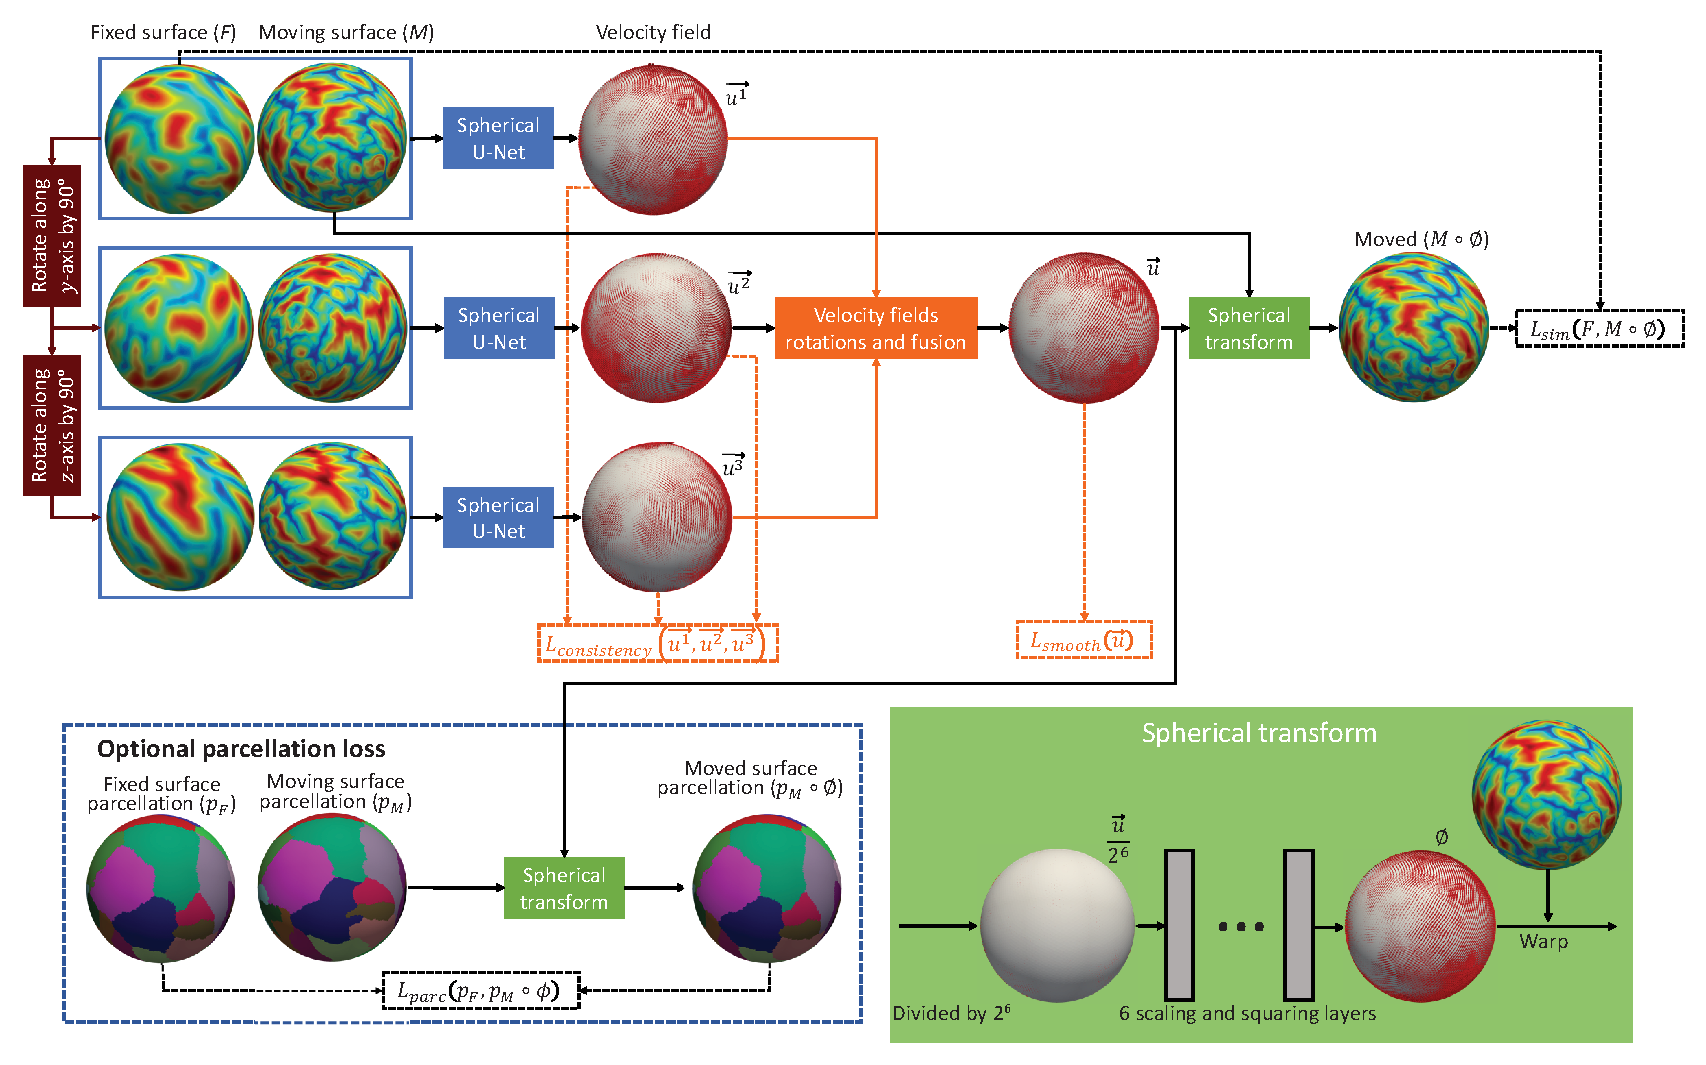
\includegraphics[width=\linewidth]{figure/network.eps}
	\caption{基于三个正交球面U-Net的S3Reg配准框架。该框架使用三个正交球面U-Net来学习三个不同方向的赤道区域的球面速度场。最终的速度场通过旋转和结合这三个不同方向的球面速度场得到。这个速度场随后会被输入到球面变形层对$M$进行变形移动,便可以得到配准到模板球面空间的配准后球面。由此利用如图所示的损失函数就可以对整个网络进行有效的训练。另外还可以利用一些辅助信息来帮助训练,例如左下方的可选的ROI分区图一致性损失。}
	\label{fig:S3Reg_network}
\end{figure}

\section{基于三个正交球面U-Net的配准框架}\label{sec:基于三个正交球面U-Net的配准框架}

\subsection{整体网络结构}
如图\ref{fig:S3Reg_network}所示,球面配准的参数函数$f_\theta(F,M)$是基于\ref{sec:基于球面U-Net的皮层分区与属性预测}\ref{sec:球面U-Net}节的球面U-Net结构。这里为了方便起见,假设$F$和$M$是包含单通道特征的球面皮层特征图,例如,sulc、curv、myelin或functional gradient density(FGD)等,尽管我们的方法可以很容易地扩展到高维特征。$F$和$M$是定义在球面$S^2$上并用正二十面体分形体\cite{fischl2012freesurfer}离散化的球重新采样得到的球面数据。球面U-Net的输入是$F$和$M$的特征串连,然后通过编码器部分重复的球面卷积和池化层对其进行编码,再由球面转置卷积和卷积层组成的解码器解码生成高分辨率的特征图。在最后一层,vertex-wise的加权用于将倒数第二层的多通道特征图映射到输出所需的2个通道,对应每一个顶点处的切平面上的速度向量。

然而,正如在背景里介绍的,球面U-Net中的1-ring卷积核最初被设计为方位角旋转不变性,这将不可避免地导致极点附近的预测结果失真,如图\ref{fig:polar_distortiion}
\begin{figure}[h]
	\centering
	\includegraphics[width=\linewidth]{figure/polar_distortiion.eps}
	\caption{使用一个球面U-Net将moving surface配准到fixed surface的配准结果。第一行和第二行分别显示了赤道附近和北极附近的配准结果。可以看到无论是网格表示的球面变形场还是用球面速度场表示的变形场,在极点附近都出现了极大的扭曲失真和拓扑错误。具体来说,第一行和第二行的moving surface的交叉三角形数量\cite{moller1997fast}分别为0和118个(总共有20480个三角形)。特别指出最后一列在靠近北极的地方显示出了较小的速度场幅度,证明了1-ring卷积核的设计在极点处固有的不连续性会导致网络无法学习到横跨极点的速度矢量。}
	\label{fig:polar_distortiion}
\end{figure}
中所展示的使用两个仿真球面配准得到的结果。造成这种失真的根本原因是,在卷积运算中,1-ring卷积核的滑动窗口在纬度上是沿0°到360°进行滑动,但在经度上只沿0°到180°进行滑动,即从北极到南极,这是为了在球面上建立一个参考方向,即本设计中的$z$轴。因此,1-ring卷积核在跨极点滑动窗口时会调转方向,这就导致了极点处的不连续性。由于预测极点区域的变形场会导致变形,而预测赤道区域的变形场则不会,我们便将球面沿$y$轴旋转了90°,并只预测赤道区域周围的变形场。这样一来,原来极点区域的变形场也可以被有效地预测出来,因为旋转后原极点区域就变成了赤道区域了。预测出变形场以后,我们再把它旋转回原来的极点区域,这样就可以得到整个球面的变形场了,从而解决了极点区域的失真问题。但是,如果只旋转球面一次,那么在某些区域的变形场会被预测两次,但在其他区域只预测一次。这将导致不同区域在网络中拥有不同的权重(2:1),甚至产生有偏差的结果。为了使权重和结果更加可靠并具有无偏,把球沿$z$轴再旋转了一次,现在变形场在大部分区域都被预测了两次,在其余的小区域被预测了三次,如图\ref{fig:S3Reg_index}
\begin{figure}[h]
	\centering
	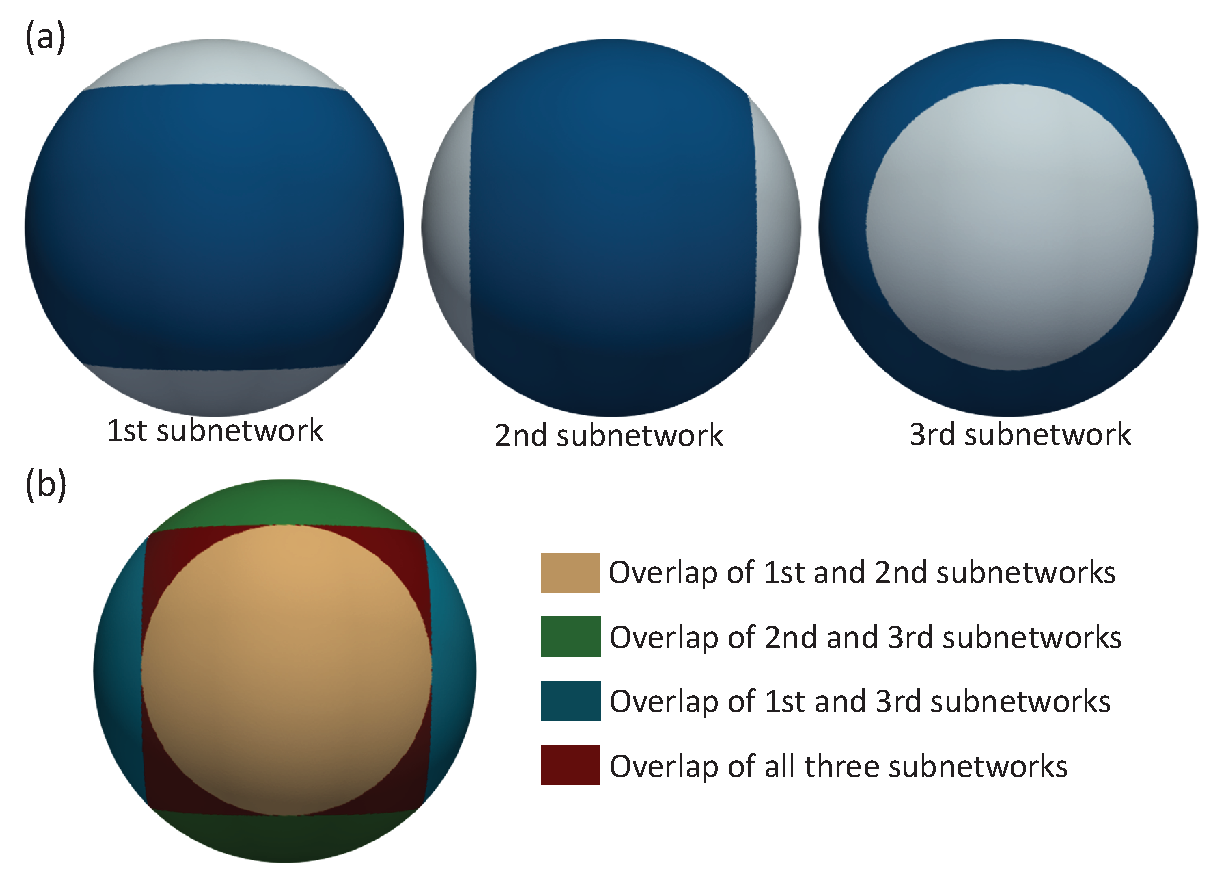
\includegraphics[width=0.67\linewidth]{figure/index.eps}
	\caption{(a) 用于解决极点失真问题的不同子网络的掩模图。深蓝色区域将被每个子网络训练和预测,而白色区域将被忽略。(b)不同子网络共同训练的重叠区域。}
	\label{fig:S3Reg_index}
\end{figure}
所示。因此,网络会更加容易地训练和学习来克服这个有偏的权重。需要注意的是,理论上任意的旋转,只要可以将极点区域移动到与原极点区域不重合的地方,都是可以的,但有些旋转把球转到了非正交区域,使得整个球的变形场合并过程很复杂,就明显不太适合。因此有些旋转方法并不有效,具体原因如下:(1)非正交的旋转造成的变形场的旋转和合并计算更加复杂;(2)不同区域之间的权重更加难以平衡。因为子网络越多,预测变形场的次数越多,理应会更准确,但是同时速度也会变慢。最后基于我们的经验,发现沿$x$、$y$、$z$轴的3个正交球面既考虑到了网络的准确性也照顾到了网络的计算复杂度,是一个最好的折中结果。

具体来讲,假设对于一个有$N$个顶点的球面${\{v_n\}}_{n=1}^N$,我们通过沿$y$轴旋转\ang{90}得到第二个球面${v_n^2}$,然后通过沿$z$轴旋转\ang{90}得到第三个球面${v_n^3}$,即:$v_n^2=R_y(\pi/2)v_n$, $v_n^3=R_z(\pi/2)v_n^2$,其中$R$是旋转矩阵,${v_n^i}$代表第$i$个球上的顶点。为了方便起见,现在也将${\{v_n\}}_{n=1}^N$表示为${\{v_n^1\}}_{n=1}^N$。然后,我们为3个方向的球面分别搭建了一个子网络,如图\ref{fig:S3Reg_network}所示,称作3个正交球面U-Net结构。每个子网络将会预测一个单独的速度场(图\ref{fig:S3Reg_network}中的$\overrightarrow{u^1}$、$\overrightarrow{u^2}$、$\overrightarrow{u^3}$),用于配准相应的旋转后的moving surface和fixed surface。然后在每个子网络中,我们设计了一个掩码用来忽略极点附近顶点的影响:$
	W(v)=\begin{cases} 
	1 & |v(z)| \leq r/\sqrt{2} \\
	0 & r/\sqrt{2} < |v(z)| \leq r  
	\end{cases}
$, 其中$r$是球$S^2$的半径,$v(z)$是顶点$v$的$z$值。图\ref{fig:S3Reg_index}(a)显示了不同子网络的掩码。图\ref{fig:S3Reg_index}(b)直观地显示了3个正交球面U-Net训练的重叠区域。由此,通过合并三个网络分别预测的球面速度场便可以得到最终的速度场$\overrightarrow{u}=\{\overrightarrow{u_n}\}_{n=1}^N$。注意这里速度场$\overrightarrow{u}$被提前合并了而不是最终再合并变形场$\phi$,这是为了减少潜在的计算冗余。

为了充分利用三个正交球面U-Net中的丰富信息,除了损失函数中的常用的特征相似性和变形场平滑项以外,我们还增加了一个新的损失函数,用来约束三个子网络生成的速度场的一致性,即希望$\overrightarrow{u^1}$, $\overrightarrow{u^2}$和$\overrightarrow{u^3}$尽可能地相似:
\begin{equation}
\begin{split}
&{\mathcal{L}}_{consistency}({\overrightarrow{u^1}},{\overrightarrow{u^2}},{\overrightarrow{u^3}}) = \\
& \frac{1}{{\left| {{O^{1,2}}} \right|}}\sum\nolimits_{n \in {O^{1,2}}} {\left| {{R_y}(\frac{\pi }{2})E_n^1{\overrightarrow{u^1}}(v_n^1) - E_n^2{\overrightarrow{u^2}}(v_n^2)} \right| + } \\
&\frac{1}{{\left| {{O^{2,3}}} \right|}}\sum\nolimits_{n \in {O^{2,3}}} {\left| {{R_z}(\frac{\pi }{2})E_n^2{\overrightarrow{u^2}}(v_n^2) - E_n^3{\overrightarrow{u^3}}(v_n^3)} \right| + } \\
&\frac{1}{{\left| {{O^{1,3}}} \right|}}\sum\nolimits_{n \in {O^{1,3}}} {\left| {{R_z}(\frac{\pi }{2}){R_y}(\frac{\pi }{2})E_n^1{\overrightarrow{u^1}}(v_n^1) - E_n^3{\overrightarrow{u^3}}(v_n^3)} \right|},
\end{split}
\end{equation}
其中,$E_n=[\overrightarrow{e_n^1}, \overrightarrow{e_n^2}]$ 是$v_n$处切平面上的一个3$\times$2的正交基,$E_n\overrightarrow{u_n}$将切平面空间的向量映射到三维空间,$O^{i,j}$表示第$i$个和第$j$个网络的重叠区域,例如:$O^{1,2}=\{n|W(v_n^1)=1 \: and \: W(v_n^2)=1\}$,其中$|O^{i,j}|$代表$O^{i,j}$中的顶点个数。


\subsection{球面变形操作}\label{sec:球面变形层}
本小节将展示用Spherical Demons\cite{yeo2009spherical}中的基本理论来导出球面变形场的表达式。变形场$\phi=\{\phi(v_n)\}_{n=1}^N$表示将一个点$v_n\in S^2 $映射到另一个点$\phi(v_n)\in S^2$。正如在背景知识部分介绍的,首先用一个静态速度场$\overrightarrow{u}$来参数化$\phi$,即$\phi=exp(\overrightarrow{u})$。静态速度场$\overrightarrow{u}=\{\overrightarrow{u_n}\}_{n=1}^N$是由上一小节的三个正交球面U-Net结构预测得到的,大小为$N\times2$。然后我们基于$\overrightarrow{u}$使用“缩放和平方”层来计算球面变形场$\phi$。第一步计算初始变形场$\phi^{(1/2^T)}$:
\begin{equation}
\phi^{(1/2^T)}(v_n)=\frac{v_n+E_n\frac{\overrightarrow{u_n}}{2^T}}{\Vert v_n+E_n\frac{\overrightarrow{u_n}}{2^T} \Vert}, 
\end{equation}
其中$T$根据经验设为6,$E_n \frac{\overrightarrow{u_n}}{2^T}$将切平面空间的速度向量映射到三维空间。这意味着$\phi^{(1/2^T)}$将移动球面上的顶点$v_n$到$\phi^{(1/2^T)}(v_n)$。请注意$v_n$和$\phi^{(1/2^T)}(v_n)$这时都是在球面上的。那么$\phi$便可以使用多个“缩放和平方”层来递归地得到,即$\phi^{(1/2^{t-1})}=\phi^{(1/2^t)}\circ\phi^{(1/2^t)}$。在数值上,对于每一次移动球面的操作,S3Reg采用重心插值法(barycentric interpolation)来插值出整个球面的变形场$\phi^{(1/2^t)}(\phi^{(1/2^t)}(v_n))$,即$v_n$先移动到$\phi^{(1/2^t)}(v_n)$,再被移到$\phi^{(1/2^t)}(\phi^{(1/2^t)}(v_n))$。通过
以上定义,在一个合理的球面配准假设下,即当$v_n$和$\phi^{(1/2^T)}(v_n)$之间的角度$\alpha$小于$\pi/2$时,该方法就可以在$\{\overrightarrow{u_n}\}_{n=1}^N$和$\{\phi(v_n)^{(1/2^T)}\}_{n=1}^N$之间建立1对1的对应关系,从而也在$\{\overrightarrow{u_n}\}_{n=1}^N$ 和$\{\phi(v_n)\}_{n=1}^N$之间建立了对应关系。因此,给定一个具有$N$个顶点的球面$\{{v_n}\}_{n=1}^N$,预测的球面变形场$\{\phi(v_n)\}_{n=1}^N$,或者等价的速度场$\{\overrightarrow{u_n}\}_{n=1}^N$,再加上一个合理的插值函数,就可以定义整个球面$S^2$上的变形场$\phi$。另外,在上述定义中,$\frac{\overrightarrow{u_n}}{2^T}$的长度等于$tan(\alpha)$,而不是Spherical Demons中的$sin(\alpha)$或球面距离$\alpha$。尽管当$\alpha$非常小的时候,这三个定义近似相等,但本论文对此的定义以较少的计算步骤在实现上更加方便和快捷。

现在对于每个移动后的顶点$\phi(v_n)$,我们选择对配准的个体球面皮层$M$进行配准,于是要计算固定球面(即模板球面$F$)上的$\phi(v_n)$处的特征值。球面插值依然选择使用重心插值法。然后S3Reg框架就可以直接在损失函数中比较$M(v_n)$和$F(\phi(v_n))$了。最后,因为球面变形层的所有运算都是可微分的,所以可以将损失函数反向传播来训练三个正交球面U-Net网络的参数。


\subsection{损失函数}\label{sec:s3reg配准网络的损失函数}
有了上述所有定义,可以将式\ref{eq:3-1}中的配准的目标函数重写为:
\begin{equation}
\begin{split}
{\mathcal{L}}(F,M,\phi) & = {\mathcal{L}}(F,M,exp(\overrightarrow{u})) \\
& = {\mathcal{L}}_{sim}(F,M\circ exp(\overrightarrow{u})) + \lambda_s {\mathcal{L}}_{smooth}(\overrightarrow{u}) \\
& \quad + \lambda_{con} {\mathcal{L}}_{consistency}(\overrightarrow{u^1}, \overrightarrow{u^2}, \overrightarrow{u^3}),
\end{split}
\end{equation}
其中$\lambda_s$和$\lambda_{con}$分别是球面变形场的平滑项权重和三个正交U-Net的速度场一致性的权重。

对于特征相似性度量,S3Reg方法选择了Spherical Demons中使用的均方差(Mean Square Distance, MSD)\cite{yeo2009spherical}和MSM配准算法\cite{robinson2014msm}中使用的相关系数(Pearson correlation coefficient, PCC):
\begin{equation}
	\begin{split}
	{\mathcal{L}}_{sim}(F,M\circ exp(\overrightarrow{u})) & = \frac{1}{N} \sum_{n=1}^{N} \Vert F(exp(\overrightarrow{u})(v_n)) - M(v_n) \Vert ^2 \\
	& - \lambda_{cc} \frac{cov(F(exp(\overrightarrow{u})(v_n)), M(v_n))}{\sqrt{\sigma_{ F(exp(\overrightarrow{u})(v_n))} \sigma_{M(v_n)}}} , 
	\end{split}
\end{equation}
其中$cov(\cdot,\cdot)$是协方差,$\sigma$是标准差,$\lambda_{cc}$是PCC项的权重,

虽然以上介绍的方法可以保证S3Reg配准框架的拓扑正确,但它仍然是基于初始变形场的,这就要求初始变形场足够小且光滑\cite{yeo2009spherical},否则,仍然有可能得到拓扑不正确的变形场,如图\ref{fig:polar_distortiion}中第二行所展示的那样。因此,在获得了切平面速度场的情况下,本论文基于1-ring卷积核提出了一个新的球面算子$\nabla_s$,见图\ref{fig:gradient_kernel},
\begin{figure}[h]
	\centering
	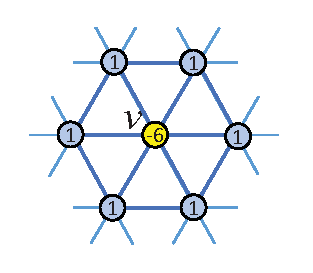
\includegraphics[width=0.35\columnwidth]{figure/gradient_kernel.eps}
	\caption{球面上近似计算球面特征梯度的算子$\nabla_s$。}
	\label{fig:gradient_kernel}
\end{figure}
用来近似球面上的特征梯度计算,从而可以显式地约束速度场的平滑性。因此,球面速度场的平滑损失为${\mathcal{L}}_{smooth}(\overrightarrow{u})=\frac{1}{N} \sum_{n=1}^{N} |\nabla_s Q(\overrightarrow{u_n}) | $,其中$Q(\overrightarrow{u_n})$代表顶点$v_n$的局部1-ring速度向量场。这个损失函数即可以惩罚$\overrightarrow{u_n}$的局部空间不平滑的变化。而且,它可以通过球面U-Net里定义的标准球面1-ring卷积层得到,在计算上非常方便快捷。

\subsection{用于辅助配准的ROI分区信息}
ROI分区图将皮层表面划分为若干个感兴趣的小的区域,即ROI,并为每个顶点分配一个ROI的标签,从而为后续大脑皮层分析提供丰富的皮层解剖区域信息。基于结构或功能特征的皮层分区图有时在配准开始前就已经存在了。它可以是由神经科学家手动标记的,也可以是算法自动得到的\cite{zhao2019spherical_isbi}。得益于S3Reg配准框架的灵活性,如图\ref{fig:S3Reg_network}所展示的,我们可以在训练过程中将分区图这样的特征信息作为额外的辅助信息整合到整个配准框架中。

直观地讲,如果一个变形场$\phi$能够将两个大脑皮层精确地配准好,那么它们的ROI分区图,即$F$和$M\circ \phi$中的ROI应该也完美地对应在一起。假设$p_F$和$p_M$是$F$和$M$的分区图,则$p_M\circ \phi$是配准后的$M$的分区图,那么我们便可以使用Dice指标来衡量每个ROI的面积重叠大小:
\begin{equation}\label{eq:Dice}
Dice(p_F^k, p_M^k \circ \phi) = 2 \frac{| p_F^k \cap (p_M^k \circ \phi)|}{|p_F^k| + |p_M^k \circ \phi|},
\end{equation}
其中$k$表示标签为$k$的ROI,$|\cdot|$表示这个ROI中顶点的数量。然后,我们定义所有$K$个ROI的平均Dice作为辅助配准的损失函数${\mathcal{L}}_{parc}$:
\begin{equation}
{\mathcal{L}}_{parc}(p_F,p_M \circ \phi) = -\frac{1}{K} \sum_{k=1}^{K} Dice(p_F^k, p_M^k \circ \phi).
\end{equation}

综上所述,用来训练S3Reg配准框架的全部损失函数可以写成:
\begin{equation}
	\begin{split}
	{\mathcal{L}}(F,M,p_F, p_M,\phi) & = {\mathcal{L}}(F,M,p_F,p_M,exp(\overrightarrow{u})) \\
	& = {\mathcal{L}}_{sim}(F,M\circ exp(\overrightarrow{u})) + \lambda_s {\mathcal{L}}_{smooth}(\overrightarrow{u}) \\
	& \quad + \lambda_{con} {\mathcal{L}}_{consistency}(\overrightarrow{u^1}, \overrightarrow{u^2}, \overrightarrow{u^3}) \\
	& \quad + \lambda_{parc} {\mathcal{L}}_{parc}(p_F,p_M \circ exp(\overrightarrow{u})) 
	\end{split}
\end{equation}
其中$\lambda_{parc}$是ROI分区图相似性的权重。



%%%%%%%%%%%%%%%%%%%%%%%%%%%%%%%%%%%%%%%%%%%%%%%%%%%%%%%%%%%%%%%%%%%%%%%%%%%%%%%%%%%
%% 第三章 基于三个正交球面U-Net的快速球面配准  实验与结果
%%%%%%%%%%%%%%%%%%%%%%%%%%%%%%%%%%%%%%%%%%%%%%%%%%%%%%%%%%%%%%%%%%%%%%%%%%%%%%%%%%%


\section{实验与结果}
为了验证本章提出的S3Reg配准方法,我们进行了一系列的实验,分别在成人和婴儿大脑皮层表面数据上配准多个皮层特征。与目前最先进的方法相比,例如,Spherical Demons\cite{yeo2009spherical},FreeSurfer\cite{fischl1999high}和MSM\cite{robinson2014msm},S3Reg展示了相当的准确度,但同时显著地减少了配准时间。为了更方便地进行试验和说明问题,本章专注于基于脑模板的配准,尽管S3Reg并不局限于此。基于脑模板的配准是将每个个体的皮层表面配准到模板表面,这是基于群体的脑皮层分析中的常见任务。我们在所有实验中都公平地使用了所有配准方法对测试数据进行个体到模板的配准。

\subsection{实验设计}
\subsubsection{数据和预处理}\label{sec:S3Reg的数据和预处理}
对于成人大脑MRI数据,我们使用了NAMIC大脑皮层数据集\cite{namic},并只在大脑左半球上进行实验,因为右半球是类似的。该数据集由39个成人大脑皮层数据组成,使用了FreeSurfer\cite{dale1999cortical}从他们各自的MR图像中重建。每个皮层表面都被映射到了球面上,表示为一个球面图像,每个顶点有2个基于皮层褶皱的几何特征,即sulc和curv\cite{fischl2012freesurfer}。和在\ref{sec:大脑皮层分区实验}节大脑皮层分区实验中介绍的一样,curv是精细度量皮层褶皱折叠模式的指标,而sulc是粗糙地度量皮层褶皱折叠模式的指标。每个皮层表面都由神经解剖学家基于主要的大脑沟回模式\cite{desikan2006automated}手动分成了35个ROI。在本实验中,我们使用FreeSurfer的大脑皮层Atlas\cite{fischl2012freesurfer}作为配准的模板,即固定的皮层表面($F$)。因为这个数据集有人工专家标记的金标准ROI分区图,使用这个数据集做实验的目的就是验证本章提出的方法在皮层表面分区上的有效性,同时本小节还会通过一些对比试验来全面展示S3Reg的各个部分的有效性。

我们还在另一个婴儿数据集上验证了本章提出的方法。这个婴儿数据集是在UNC医院采集的,有102个1岁左右的婴儿大脑MR图像数据。婴儿大脑皮层表面使用了婴儿专用的pipeline\cite{li2015construction,li2014measuring,wang2018volume}(iBEAT V2.0 Cloud, http://www.ibeat.cloud/)进行重建,然后每个皮层表面被映射到了球面上。每个皮层表面都含有多模态的特征,包括2个几何形态学特征,即sulc和curv,另外还有2个功能特征,即髓鞘含量(Myelin content, 简称myelin)和功能梯度密度(functional gradient density,简称FGD)。接着这些婴儿大脑皮层表面使用了\ref{sec:大脑皮层分区实验}中的方法得到了自动的ROI分区图。Myelin和FGD都是可靠且有意义的功能特征,与皮层功能区域密切相关\cite{glasser2016multi}。Myelin是使用T1w/T2w图像得到的。FGD使用了以下方法计算得到。首先在婴儿自然睡眠期间采集得到婴儿静息态fMRI(resting-state fMRI, rfMRI)数据。然后除了使用常规的HCP fMRI处理步骤\cite{glasser2013minimal}外,我们还特别采用了以下策略\cite{hu2020disentangled}来处理这些fMRI数据:(1)在原生图像空间中完成功能信号的一次性重采样和去噪;(2)基于深度学习的噪声成分去除,以实现快速鲁棒的fMRI去噪,然后提取了皮层表面各顶点的fMRI时间序列,再使用\cite{huang2020construction,gordon2016generation}中的方法在皮层表面计算出FGD图。另外,用于配准该数据集的模板是由其他83个年龄相近的个体使用Spherical Demons\cite{yeo2009spherical}经过group-wise配准后平均得到的。由于这个婴儿数据集没有金标准的ROI分区图,该组实验的目的即在于额外地验证本章方法在多模态特征配准上的泛化能力。

\subsubsection{传统方法的实现细节}\label{sec:配准的基准方法}
本实验使用了Spherical Demons (https://sites.google.com/site/yeoyeo02/software/sp
hericaldemonsrelease)、MSM (fsl/6.0.0中的MSM命令)和FreeSurfer (FreeSurfer/7.1.0)的官方代码来进行它们的实验。在这些非刚性配准方法开始之前,我们使用了一个基于旋转的刚性配准来完成初始化,就像在Spherical demons\cite{yeo2009spherical}和FreeSurfer\cite{fischl2012freesurfer}中做的一样,即沿着每个轴进行穷举搜索,共进行了4轮搜索,每轮的搜索范围分别为[-64°, 64°]、[-32°, 32°]、[-16°, 16°]和[-8°, 8°]。用于评价旋转后的球面和固定球面的特征相似度的指标是sulc的均方误差。然后我们在默认参数下运行Spherical Demons和FreeSurfer,即将两个球面在4个级别的正二十面体分形球面上进行配准(4,5,6,7级,分别有2562,10242,40962,163842个顶点),分别用来配准sulc,sulc,sulc和curv。对于功能特征的配准,基于sulc配准的结果,再在第6级分辨率上使用了与curv相同的超参数配置来配准婴儿脑皮层表面的功能特征。对于MSM,由于默认参数不能得到满意的结果,我们在每个数据集上使用了不同的调参后优化的参数,即将它默认的正则化项参数变大,输入平滑项变小了一点。对于2个几何特征(先是sulc,然后是curv),仍然是默认地运行在4个分辨率级别(sulc为4,4,5,6,然后curv为4,5,5,6),每个级别使用了3次迭代。对于功能特征,与Spherical Demons和FreeSurfer一致,MSM使用了与curv相同的配置,但只在第6级分辨率上运行。为了与我们的方法有一个公平的比较,上述传统方法的实验都在英特尔酷睿i7-8700 CPU上运行。

\subsubsection{本论文提出的S3Reg的实现细节}
本论文提出的S3Reg配准框架是使用PyTorch\cite{paszke2017automatic}工具包实现的,并使用Adam优化器\cite{kingma2014adam}和1e-5的学习率训练了100个epochs。sulc和curv的特征值首先通过减去平均值并除以标准差来进行归一化处理。与一般的单次3D图像配准不同的是,皮层表面配准更倾向于使用由粗到细的方式在多个分辨率下配准多个特征,正如在以前的方法\ref{sec:配准的基准方法}中执行的那样。因此,S3Reg也使用了由粗到细的多层次配准算法,作为默认的S3Reg配准算法,即在4个分辨率级别(3,4,5,6)分别训练4个模型,作为默认的几何特征配准模型,称为S3Reg-multi-sulc-curv,分别用于配准sulc,sulc,sulc和curv。注意这4个模型是单独分开进行训练的。具体来讲,我们首先在分辨率比较低的球面上训练一个用于配准sulc特征的低分辨率模型(3级)。该网络训练完成后,我们会保存该模型,并预测出在第3级分辨率上配准sulc的变形场。然后将第3级的变形场上采样到第4级,并用于配准第4级的皮层表面。然后,在第4级训练新的模型,用于配准在刚刚移动后得到的表面上的新的特征。随后重复这个过程,直到第6级配准curv完成。对于从当前分辨率到下一个分辨率变形场的上采样操作,S3Reg依然使用重心插值法去生成新的移动顶点,然后再将它们映射到球面上。对于球面上的下采样操作,S3Reg提取低分辨率球面上的顶点(及其特征),便可以从高分辨率球面上得到下采样的球面。在这个下采样过程之前,我们没有应用任何平滑处理,这一点不同于MSM\cite{robinson2014msm},因为我们发现下采样过程中的球面特征平滑操作对最后的结果并没有显著影响。为了显示多级分层次配准的优越性,我们另外训练了几个模型,只在第6个分形体球面上配准sulc,称作S3Reg-single-sulc模型,然后在第6级上再配准curv,叫作S3Reg-single-sulc-curv。为了进一步显示可选的辅助ROI分区图所带来的改进,在S3Reg-multi-sulc-curv的最后一级增加ROI分区图一致性损失函数便可得到S3Reg-multi-sulc-curv+parc模型。对于功能特征,S3Reg依然使用与Spherical Demons和MSM中相同的配准策略。

本章的实验使用了60\%的数据进行训练,10\%的数据进行验证,30\%的数据进行测试。用于训练每一级模型的$\lambda_{cc}$和$\lambda_{con}$始终为1。训练每一级配准sulc模型的$\lambda_s$分别为8、10、12、16,第6级的curv、myelin和FGD为40。$\lambda_{parc}$在第6级是10。所有实验都在一台拥有NVIDIA RTX2080 Ti GPU和Intel Core i7-8700 CPU的PC上运行。

\subsubsection{评价指标}\label{sec:配准的评价指标}
为了定量评估配准性能,本实验采用公式\ref{eq:Dice}计算了广泛使用的ROI分区图的Dice指标\cite{dice1945measures}。由于更好的配准会让解剖边界达到更高的一致性,因此更大的Dice值表明更好的配准结果。需要注意的是,这里的Dice是直接基于两个配准后的ROI分区图计算的,而不是手工标记的分区图和使用额外分类器基于配准后的特征预测得到的分区图之间的Dice。因为本章内容更关心配准方法的公平比较,而不想牵扯到其他任何的分类器。此外,我们还计算了配准后两个皮层表面特征图的平均绝对误差(Mean Absolute Error, MAE)和皮尔逊相关系数(PCC),用来直接评价配准后特征的对齐情况。因此,较高的PCC和较低的MAE都表示更好的配准结果。因为配准后所有的皮层表面都应该在同一个空间,我们就计算了测试集中的任意两个配准后的皮层表面的以上指标,并展示了它们的平均结果。另外由于损失函数也使用了MSD和PCC来训练网络,这里的MAE和PCC只是为评价组内数据的空间归一化准确度提供一个额外的指标。作为一个更无偏的衡量标准,Dice是一个更可靠更有说服力的评价指标,可以用来决定哪一种方法具有更加优秀的性能\cite{rohlfing2011image}。

\begin{table}[h]
		\caption{在NAMIC数据集上的配准性能比较。*表示与S3Reg-multi-sulc-curv相比有统计学上的显著差异($p<$0.05)。粗体和斜体数字分别表示最好和第二好的结果。}
		\label{tab:NAMIC成人数据集的配准结果比较}
		\centering
		\zihao{-5}
		\begin{tabularx}{\linewidth}{lccccccc}
			\Xhline{2\arrayrulewidth}
			&       \makecell{PCC of\\ sulc}         &     \makecell{PCC of\\ curv}          &     \makecell{MAE of\\ sulc}  &         \makecell{MAE of\\ curv}     & Dice                     & CPU时间 & GPU时间 \\
			\hline
			S3Reg-single-sulc           &   0.7025*	        &   0.1820*	        &  3.0554*	       &  0.1761*	     &   0.7677*	        &    \textbf{3.5s} & \textbf{1.1s} \\
			S3Reg-single-sulc-curv      &	0.7662*	        &  0.3658*           &  	2.6633*         &   0.1529*	     &   0.7956*	        &   \textit{6.7s}  &\textit{4.6s}   \\
			MSM\cite{robinson2014msm}                       &	0.7972*	        &   \textit{0.4393}  &   2.5034*	       &   0.1409	     &   0.7963*	        &   8min           &  -            \\
			Spherical Demons\cite{yeo2009spherical}	        &    0.8005*         &	0.4026*          &   	2.4523*	   &   0.1467*	     &   \textit{0.8084} &   1min           & -             \\
		   FreeSurfer\cite{fischl2012freesurfer}     &    0.7991*         &	0.4091*          &   	2.4620*	   &   0.1461*    &   0.8010* &   30min       & -       \\
			S3Reg-multi-sulc-curv	    &   \textit{0.8196}	&   0.4338           &  	\textit{2.2859} & \textit{0.1408}	 &   0.8074	        &   13.0s          &   9.1s        \\
			S3Reg-multi-sulc-curv+parc	& 	\textbf{0.8338*}	& \textbf{0.4487*}	& \textbf{2.1542*}  & \textbf{0.1400}  & \textbf{0.8108*}  &   13.0s          &   9.1s        \\		
			\Xhline{2\arrayrulewidth}
		\end{tabularx}
\end{table}

\subsection{成人大脑皮层表面的配准结果}

表\ref{tab:NAMIC成人数据集的配准结果比较}列出了不同方法在NAMIC数据集上的配准结果。可以看到S3Reg-multi-sulc-curv+parc在所有指标上都取得了比其他方法更好的结果,这里注意S3Reg-multi-sulc-curv+parc模型在测试过程中并没有使用ROI分区图,只是在训练阶段使用了分区图来辅助训练而已,这说明ROI分区图和由粗到细的多分辨率配准方式确实有助于提高配准效果。唯一的一个例外,即curv的MAE,与S3Reg-multi-sulc-curv和MSM没有表现出显著的差异,这可能是因为S3Reg-multi-sulc-curv和MSM已经达到了curv的MAE性能的下限。在没有辅助的分区图信息的情况下,默认的S3Reg模型,即S3Reg-multi-sulc-curv,在sulc上实现了比MSM和Spherical Demons更好的配准效果,这得益于特别设计的与评价指标相匹配的MSD和PCC损失函数。另一方面,MSM在curv上获得了更好的配准效果,这是因为只有MSM是基于sulc配准结果在不同分辨率上多次进行curv配准的。在Dice方面,由于Spherical Demons最初是基于NAMIC数据集开发验证的,并在这个数据集上进行了配准和分区的实验,因此Spherical Demons中的默认参数有助于它在这个数据集上获得更好的Dice结果,最后的结果也验证了这个想法,即Spherical Demons的Dice值十分接近默认的S3Reg模型。

图\ref{fig:registration_roi_wise_dice}
\begin{figure}[t]
    \centering
    	\includegraphics[width=\columnwidth]{figure/roi-wise_dice.eps}
	\caption{ROI-wise配准Dice箱形图。}
	\label{fig:registration_roi_wise_dice}
\end{figure}
显示了不同配准方法的ROI-wise的Dice值,可以看到S3Reg-multi-sulc-curv+parc模型在34个区域中的25个区域都获得了最好的结果。在剩下的9个次优区域中,只有4个区域(cuneus cortex, paracentral lobule, pars orbitalis, temporal pole)显示出了显著差异。尽管如此,由于这些方法都提供了灵活的正则项或平滑项参数用来权衡配准精度与变形场的平滑度,因此结果还是可以依据参数微调的。然而,在运行时间上,本章提出的S3Reg配准算法仅需要
\begin{figure}[h]
	\centering
	\includegraphics[width=0.62\linewidth]{figure/NAMIC_ATLAS.eps}
	\caption{配准后得到的NAMIC数据集的平均皮层表面特征图和对应的方差图。像之前的工作\cite{lyu2019hierarchical}一样,这里也展示了方差图的平均方差及其标准差并标注在了每个方差图的下方。}
	\label{fig:NAMIC_ATLAS}
\end{figure}
学习一个全局优化函数来配准所有的皮层表面,因此显著提高了计算效率。即使完全训练S3Reg模型需要大约12个小时,但与其他方法相比,在使用相同的CPU情况下,它在测试的时候只需要13秒。当进一步利用GPU的高算力优势时,S3Reg将配准时间降低到了10秒以内。需要注意的是,与其他深度学习应用相比,S3Reg在GPU上的速度相比CPU上的速度提升并不是很大。这是因为配准中最耗时的步骤,即特征和变形场的重心插值过程,需要在球面上进行三角形的穷举搜索,这个过程在GPU上的速度依然还是比较慢的。

图\ref{fig:NAMIC_ATLAS}展示了NAMIC数据集中的所有测试对象在使用不同方法配准到FreeSurfer皮层模板后的组平均特征图和方差图。可以看到S3Reg在许多区域呈现出更加清晰的折叠模式,并且在所有测试数据中获得了比较低的方差,这表明这两个皮层结构特征被很好地配准对齐了。图\ref{fig:example_registration}
\begin{figure}[h]
	\centering
	\includegraphics[width=0.77\linewidth]{figure/example_registration.eps}
	\caption{将moving surface配准到atlas surface的例子。}
	\label{fig:example_registration}
\end{figure}
提供了一个使用不同方法进行配准的代表性例子。可以看到对于sulc和curv的配准,所有方法都获得了非常相似的结果。而对于该皮层表面的分区图,S3Reg模型在训练过程中利用了分区图的辅助信息,于是获得了更好的与模板对齐的结果。


\subsection{婴儿大脑皮层表面配准的结果}
表\ref{tab:婴儿皮层表面的配准结果}和图\ref{fig:infant_ATLAS}分别显示了使用不同方法基于皮层结构特征sulc和curv将皮层表面配准到模板皮层表面后,测试数据集里的婴儿皮层表面的定量的组归一化结果和定性的组平均和方差图。
\begin{table}[h]
	\caption{基于结构特征的婴儿大脑皮层表面的配准结果。*表示与S3Reg相比有统计学上的显著差异($p<$0.05)。}
	\label{tab:婴儿皮层表面的配准结果}
	\centering
	\zihao{5}
	\begin{tabularx}{0.9\columnwidth}{X<{\centering} X<{\centering} X<{\centering} X<{\centering}}
		\Xhline{2\arrayrulewidth}
			& Spherical Demons &	MSM	& S3Reg  \\
		\hline
			PCC of sulc &	0.6982±0.0521* &	0.7103±0.0431*  &	\textbf{0.7359±0.0526}  \\
			PCC of curv &	0.2749±0.0811*	&  \textbf{0.3268±0.0762*}  &	0.2955±0.0810\\
			MAE of sulc &	2.7669±0.3528* &	2.6660±0.3168* &	\textbf{2.3730±0.3362}  \\
			MAE of curv &	0.1933±0.0205* &	\textbf{0.1790±0.0189*} &	0.1853±0.0197\\
			Dice&	0.7858±0.0583 &	0.7659±0.0552* &	\textbf{0.7903±0.0566} \\		
		\Xhline{2\arrayrulewidth}
	\end{tabularx}
\end{table}
\begin{figure}[h]
	\centering
	\includegraphics[width=0.68\linewidth]{figure/infant_ATLAS.eps}
	\caption{使用不同方法配准后的婴儿大脑皮层结构特征的组平均图和方差图。}
	\label{fig:infant_ATLAS}
\end{figure}
结果与NAMIC数据集非常一致,即S3Reg在sulc的配准上得到了更好的结果,而MSM在curv的配准上获得了更好的结果,Spherical Demons和S3Reg都获得了最高的Dice。从定性结果看,在许多ROI中,如rostral middle frontal和gyrus and temporal-occipital junction cortex,本章提出的S3Reg呈现出了更清晰的皮层折叠模式,这表明每个个体之间都实现了更好的与模板表面的配准。

此外,为了验证本章提出的方法的泛化能力和可扩展性,基于第6级正二十面体分形球面的sulc配准结果,我们分别配准了myelin和FGD。注意到使用不同方法得到的基于结构特征的配准结果作为初始配准球面可能会影响到最后的功能特征的配准结果,因此为了在不同的方法之间有一个公平的比较,实验选择了Spherical Demons的sulc配准结果作为所有方法的初始配准结果,因为它直接提供了一个第7级的高分辨率的皮层表面与配准好的皮层特征。这里要注意无论初始化方法是哪一个,最后的结果应该都是一样的。表\ref{tab:婴儿皮层表面功能特征配准结果}
\begin{table}[h]
		\caption{基于婴儿皮层表面功能特征的配准结果比较。表中所有的结果均有显著性差异。}
		\label{tab:婴儿皮层表面功能特征配准结果}
		\centering
		\zihao{5}
		\begin{tabularx}{0.9\columnwidth}{X<{\centering} X<{\centering} X<{\centering} X<{\centering}}
			\Xhline{2\arrayrulewidth}
			& Spherical Demons &	MSM	& S3Reg  \\
		    \hline
			PCC of myelin              &	0.6929±0.1127	 &  0.6362±0.1225 &	\textbf{0.7196±0.1082} \\
			MAE of myelin              &	0.1076±0.0312    &	0.1127±0.0327 &	\textbf{0.0970±0.0301} \\
			PCC of FGD    &	0.4340±0.0867    &	0.4115±0.1163 &	\textbf{0.5154±0.0740} \\
			MAE of FGD	   &    0.0874±0.0132    &	0.0914±0.0180 &	\textbf{0.0741±0.0121} \\	
			\Xhline{2\arrayrulewidth}
		\end{tabularx}
\end{table}
\begin{figure}[h]
	\centering
	\includegraphics[width=0.73\linewidth]{figure/myelinandgrad.eps}
	\caption{第一行和第三行显示了原始图谱的myelin和FGD图,以及使用不同方法配准后得到的大脑皮层表面平均后生成的新图谱。第二行和第四行为其对应的方差图。}
	\label{fig:myelinandgrad}
\end{figure}
总结了功能特征驱动的婴儿大脑皮层表面配准结果。在与配准curv时参数相同的情况下,Spherical Demons和MSM对新功能特征的泛化程度明显较低,而S3Reg仍然取得了
显示了测试集的myelin和FGD在使用不同方法配准后的平均特征图和方差图。可以看出,S3Reg呈现出比原始模板、Spherical Demons和MSM都更加清晰锐利的平均图,说明在这组数据的配准中,个体到模板的配准是很精准的。由于这个平均图可以看作是一个新的群体模板,因此本章提出的S3Reg所呈现的更清晰的新模板对后续的分析也会大有裨益。


\subsection{异常大脑皮层表面的配准结果}
由于上述结果都是基于健康的大脑皮层,因此这一小节进行了一个额外的实验,配准阿尔茨海默病(ADNI)数据库\cite{jack2008alzheimer}中的皮层表面,用来在前瞻性研究中更好地验证本章提出的方法在异常大脑上的表现。这个实验直接应用了之前使用的成人数据训练好的模型,将ADNI数据集中的皮层表面配准到FreeSurfer的平均模板上。注意到我们并没有使用任何ADNI的数据来训练或微调模型。实验的数据由ADNI-1数据集的428名参与者组成,分为年龄相匹配的2组,分别是健康对照组(Health Control, HC)(n=229,平均年龄:76.0$\pm$5.1岁,48\%为女性)和阿尔茨海默病组(Alzheimer's Disease, AD)(n=199,平均年龄:75.6$\pm$7.3岁,48.5\%女性)。我们选择使用了每个受试者的第一次扫描的大脑MRI数据,这些数据都是由1.5T磁共振扫描仪采集得到的并且具有足够高的图像质量。所有的皮层表面都由FreeSurfer重建好\cite{fischl2012freesurfer},并进一步映射到球面上。考虑到FreeSurfer在神经影像领域的流行度,本实验将我们的方法与FreeSurfer的配准工具(mris\_register)进行了比较。具体来讲,从相同的球面映射的大脑皮层数据开始,我们分别使用FreeSurfer和S3Reg将它们配准到FreeSurfer平均(fsaverage)皮层表面\cite{fischl2012freesurfer}。然后使用FreeSurfer中的一般线性模型(General Linear Model, GLM)对两组配准好的大脑皮层的皮层厚度属性进行逐个顶点的比较,就可以分别为FreeSurfer和S3Reg生成显示AD和HC之间统计显著性差异的皮层表面图,如图\ref{fig:ADVSHC}
\begin{figure}[h]
	\centering
	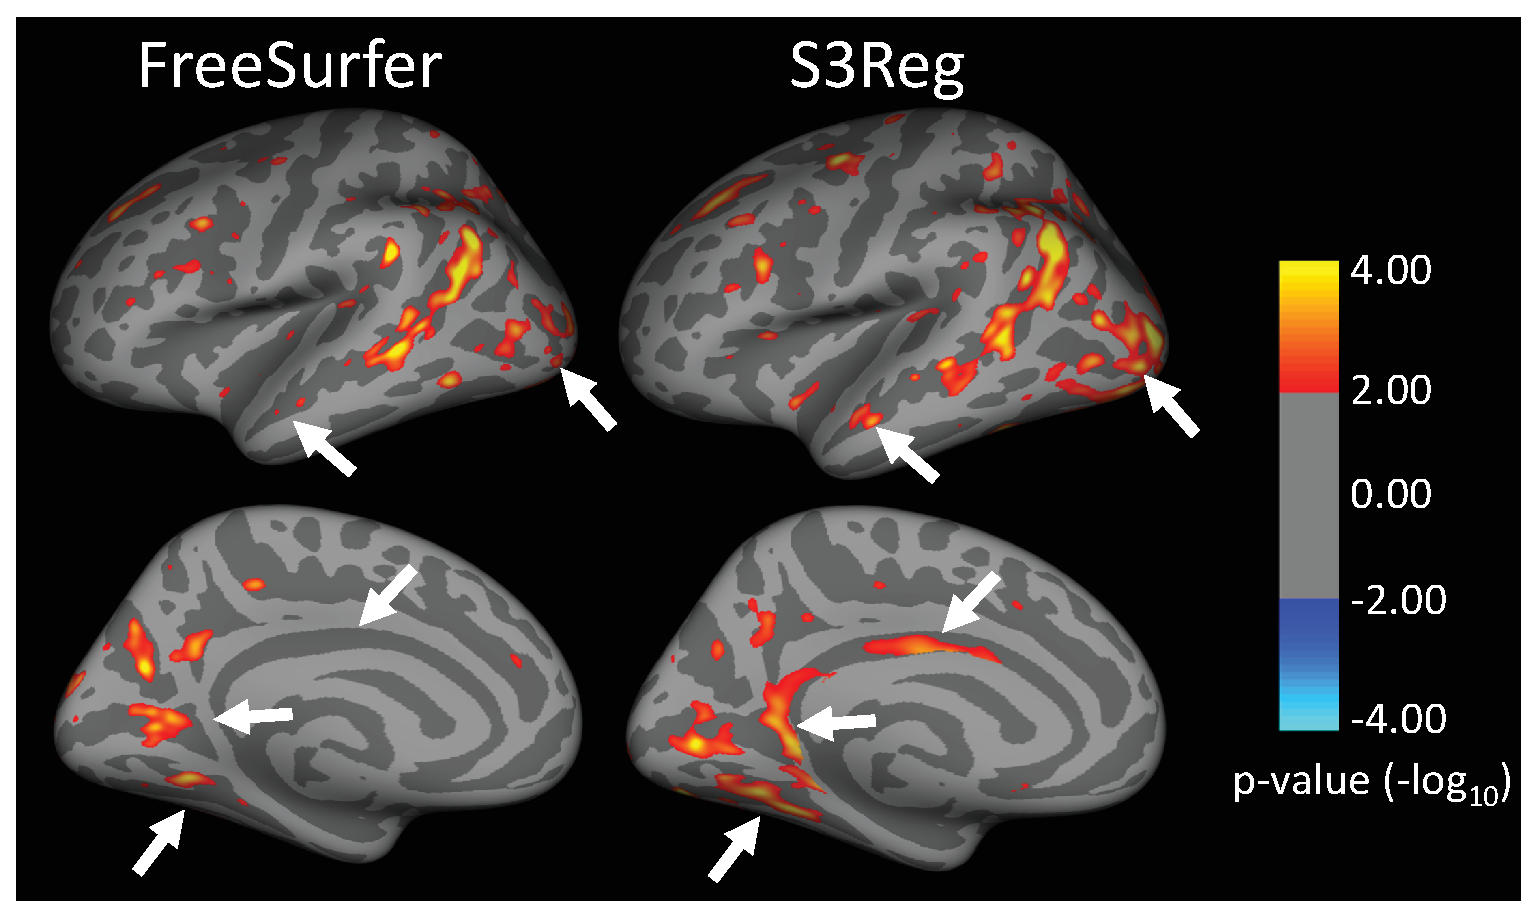
\includegraphics[width=0.8\linewidth]{figure/ADVSHC.eps}
	\caption{基于FreeSurfer和S3Reg得到的阿尔茨海默病(AD)和健康对照组在大脑皮层左半球的皮层厚度差异图。结果已经使用了$q~rate$为0.05的多重比较校正。皮层颜色显示了$p$值的对数值($-log_{10}$)。较暖的颜色(正值)代表AD中具有统计学意义的显著变薄区域;较冷的颜色(负值)代表AD中具有统计学意义的皮层增厚的区域。}
	\label{fig:ADVSHC}
\end{figure}
所示。两种配准方法的结果均显示了在AD组内,中侧颞叶皮层(lateral temporal cortex)、下顶叶皮层(inferior parietal cortex)、背上额回(dorsal superior frontal gyrus)、外侧和内侧枕叶皮层(lateral and medial occipital cortex)的皮层明显变薄。然而,如箭头所指,我们的S3Reg比FreeSurfer揭示了更多更大的显著性变薄区域,特别是在颞上沟(superior temporal sulcus)、侧枕部皮层(lateral occipital cortex)、背上额叶回(dorsal superior frontal gyrus)、纺锤形回(fusiform gyrus)、副海马回(parahippocampal gyrus)、峡部(isthmus)和后扣带皮层(posterior cingulate cortex)。这些结果表明,S3Reg更准确地配准了不同个体的皮层表面,因此在疾病检测方面更加有效,计算效率也更高。同时,本章开发的S3Reg算法只需要10s即可完成一次配准,而FreeSurfer则需要30min。

\section{讨论}
本章提出了用于球形皮层表面配准的新型S3Reg框架。受益于基于CNN的深度学习技术和端到端的无监督学习架构,S3Reg配准算法取得了的令人欣喜的表现,为多模态皮层特征配准提供了超快、拓扑保证、准确和灵活的结果。然而作为一个多功能的通用算法,仍有几个潜在的问题值得讨论。

首先,由于多模态MRI数据的配准是一个非常复杂的问题,而且现在领域内对于皮层配准的最佳策略还没有达成共识\cite{robinson2014msm,glasser2016multi},因此非常需要一个灵活的配准框架,使得大脑皮层配准可以很容易地扩展到其他多模态特征(如结构、功能、功能连接或它们的组合)。我们相信本章开发的方法将会鼓励网络利用强大的深度学习能力,自动学习不同的特征组合和不同区域的权重来自动发现最佳的配准策略。然而,本章的大部分重点依然是在多模态特征的顺序配准上,仅使用了很多潜在应用场景中的一小部分来初步验证了方法的准确性和速度。需要注意的是,本文中配准大脑皮层解剖学结构所使用的特征和它们的顺序(分别为3、4、5、6级的sulc、sulc、sulc、curv)借鉴自流行的配准策略\cite{yeo2009spherical,glasser2016multi,robinson2014msm,fischl1999high}。这个策略是经验性的,并没有被证明是最优解。在未来的工作中,我们将进一步验证和探索使用不同的配准策略和高维特征来发现更具有生物学意义的配准方式。由于S3Reg框架是非常通用的,从其他MR成像模式衍生出来的皮层特征,例如,从DWI计算得到的皮层扩散性和纤维连接性\cite{li2010cortical,li2015spatiotemporal,rekik2017joint}、从特定任务的功能MRI(task functional MRI, tfMRI)计算出的任务激活图,都可以方便地整合进本章提出的方法。此外,除了皮层表面,S3Reg算法框架也适用于配准其他具有球形拓扑结构的表面数据,例如,皮层下结构的形状和连接特征。

关于参数的选择,我们发现平滑项($\lambda_s$)的权重越大则越容易生成平滑的变形场,但会造成较低的特征相似性,而特征相似性项的权重越大,将会导致更好的特征对齐,但可能造成一个不太平滑甚至拓扑不正确的变形场。在速度场一致性损失($\lambda_{con}$)方面,权重1.0足以保证不同子网络的预测之间的一致性,进一步增加权重对结果没有明显影响。但是,如果权重低于1.0,则会导致预测结果之间的不一致。ROI分区图相似性损失($\lambda_{parc}$)与速度场一致性损失有着相似的模式。我们还发现分区图相似性用来提高Dice指标的权重上限为10.0。关于PCC和MSD项,实验发现无论使用其中的哪一项结果都很相似。这是因为这两个相似度指标都与特征的对齐程度呈正相关,无论哪一个都能有效地检测到moving surface与fixed surface的相似度。因此本章实验将相关系数损失的权重($\lambda_{cc}$)设置为1.0。

在速度提升方面,这里需要强调的是整个过程都是单纯地基于配准过程的比较,即在神经影像处理pipeline中的起点和终点相同,这意味着对于整个神经影像分析pipeline来说,本章提出的方法的速度提升也是整个pipeline的速度提升。另一方面,由于传统方法没有GPU版本的代码,本章提出的方法利用了GPU的优势,将配准过程进一步加快到只需要不到10秒。由于近几年GPU在计算方面越来越流行,这对神经影像研究领域来说是一个非常有价值的贡献,可以极大地促进大规模神经影像数据的分析。

另外一个值得注意的点是,成人和婴儿大脑皮层表面之间确实存在差异,如果直接将在一个数据集上训练的模型应用到另一个数据集上,显然会降低配准精度。这是因为婴儿的大脑皮层表面与成人的皮层表面在皮层大小、形状、折叠模式和功能特征等方面,都存在较大的差异\cite{li2015construction}。此外,这两个数据集之间也存在不同扫描仪的影响,这是由不同的扫描仪、成像协议和图像处理pipeline造成的。因此,将在成人或婴儿数据集上训练的模型直接应用到婴儿或成人数据集上,与在目标数据集上重新训练或微调的模型相比,不可避免地会导致一定程度的性能下降。这也是一个基于CNN的深度学习方法的普遍且重要的问题\cite{shen2017deep}。尽管如此,我们在一个独立的成人数据集上展示了本章提出的方法的性能,即在多个中心收集的ADNI数据集上。结果表明,本章提出的方法在不同成人数据集上的泛化能力是令人满意的,即使这仍然需要在未来的大规模神经影像研究中进一步地验证。最后,为了提高本章开发的S3Reg配准模型的泛化能力,我们可以加入一些数据集自适应技术\cite{he2020self}或跨数据集不变特征提取技术\cite{zhong2020dika}来解决一部分成人和婴儿数据集之间的差异问题,或者采用一些数据结合技术\cite{zhao2019harmonization}来去除扫描仪影响,然后再训练配准网络。这样一来,应该就可以得到一个在不同的数据集上都能很好地工作,泛化能力更强的配准模型。

\section{本章小结}
本章提出了一个基于深度学习方法的多功能大脑皮层表面配准框架S3Reg,用于在球面空间上进行快速灵活的皮层表面配准。本章的实验结果表明S3Reg不需要金标准的球面变形场,只利用端到端无监督学习的特点,再结合3个互补的正交球面U-Net,便可以有效地解决球面配准上的极点变形问题。为了保证球面变形场的拓扑属性,本章开发了一个新的球面“缩放和平方”可微分层用于静态速度场的积分以得到diffeomorphism的球面变形场。如结果中所示,本章提出的S3Reg可以灵活地结合来自结构和功能图像的多模态特征进行皮层表面配准。更重要的是,与目前最好的非深度学习方法相比,S3Reg运行速度更快,同时还能获得更高的配准精度,使其更适合大规模神经影像数据分析。此外,本章开发的方法不受相似度指标和平滑度约束的选择影响,从而为球面配准提供了更多的选择和潜在的研究方向,也为其他亏格为0的器官和一些以球面数据为对象的计算机视觉任务提供了新的研究方向。






%%%%%%%%%%%%%%%%%%%%%%%%%%%%%%%%%%%%%%%%%%%%%%%%%%%%%%%%%%%%%%%%%%%%%%%%%%%%%%%%%%%
%% 第四章 同时分区与配准
%%%%%%%%%%%%%%%%%%%%%%%%%%%%%%%%%%%%%%%%%%%%%%%%%%%%%%%%%%%%%%%%%%%%%%%%%%%%%%%%%%%



\chapter{基于球面神经网络的大脑皮层同时分区与配准}\label{sec:基于球面神经网络的大脑皮层同时分区与配准}

\ref{sec:基于球面U-Net的皮层分区与属性预测}和\ref{sec:基于三个正交球面U-Net的快速球面配准算法}分别介绍了本论文在皮层表面配准和分区任务上做的两个连续的但独立的研究工作,它们都是大脑皮层表面神经影像分析中的两个重要的基础任务。大脑皮层表面配准是估计一个变形场,用来对齐来自不同个体的大脑皮层的结构或功能属性,并建立不同个体之间或不同时间点之间的vertex-wise的皮层对应关系\cite{fischl1999high,yeo2009spherical,zhao2020unsupervised},从而促进后续的比较分析,例如,不同群体之间的横向比较或同一个个体不同时间点之间的纵向比较。大脑皮层表面分区需要学习皮层的特征与解剖或功能区域之间的非线性映射关系,从而将皮层分成不同的ROI\cite{desikan2006automated,zhao2021sphericalDeformable,wu2018registration}。一般来讲,这两个任务通常是独立进行的\cite{li2019computational},即配准过程只关心配准,分区过程也只追求分区的准确度,但这样明显忽略了它们之间存在的内在密切关系。这个密切关系是指,它们都依赖于有效的皮层特征表达,一个用于预测变形场,另一个用于预测ROI标签,这说明它们在使用不同的视角探索和学习皮层属性。因此同时进行分区和配准可以更好地规范整个学习过程,获得更有意义和鲁棒的特征表达。简而言之,这两个任务可以互相帮助并互相提升对方的性能表现。具体来讲,对于分区任务来说,借助皮层表面配准任务建立好的顶点对应关系,一个大脑皮层或模板皮层上的手动标记的ROI分区图可以很容易地传递到另一个新的皮层上,从而为分区任务生成更多的训练数据,以帮助分区任务更好地学习从属性到ROI标签的映射。反过来,对于配准任务来说,除了皮层结构和功能属性外,分区任务得到的ROI分区图的边界信息也可以作为额外的辅助配准信息,从而更好地学习从特征到变形场的映射。

因此,本章利用大脑皮层的球形拓扑结构,基于\ref{sec:基于球面U-Net的皮层分区与属性预测}开发的球面卷积神经网络的基本操作,探讨研究了同时进行皮层表面配准和分区的想法。为了提取更有效的皮层特征,本章设计了一个共享编码器用来学习两个任务共享的皮层属性高级特征。然后,训练了两个针对特定任务的解码器分别进行配准和分区。另外,本章还进一步地利用两个任务之间的显示联系,由此设计了一个新的ROI分区图相似性损失函数。这个损失函数会约束配准后的moved surface的预测分区图与fixed surface(即atlas surface)的手动标记的分区图相匹配,从而为配准任务提供额外的ROI边界一致性的监督信息。相反,这个损失函数也可以被认为是一种有效的数据增强方法,为未被人工标记过的皮层表面生成伪ROI分区图,这样就可以给分区网络提供更多的训练数据,从而帮助分区网络进行半监督学习\cite{xu2019deepatlas}。因此,与单独训练的网络相比,这两个任务可以相互帮助、相互指导、相互提升对方的性能,尤其是在只有少量的人工标注数据的情况下。因此,这个工作对于只有少量人工标注的大脑皮层数据集的处理与分析有着十分重要的意义。

\section{大脑皮层同时分区与配准的方法}\label{sec:大脑皮层同时分区与配准的网络结构}
本章的主要目标是训练一个同时配准和分区的网络(Joint Registration and Parcellation Network, JRP-Net),该网络会根据给定的皮层表面属性图生成其ROI分区图并同时得到它到atlas的变形场,其次的目标是希望使用更少的人工标注数据得到更准确的结果。为了达到这个目标,本章提出的JRP-Net方法框架如图\ref{fig:jrp_network_archi}
\begin{figure}[h]
	\centering
	\includegraphics[width=\linewidth]{figure/jrp_network_archi.eps}
	\caption{用于大脑皮层表面同时配准和分区的JRP-Net网络框架。输入的皮层表面由两个结构特征表示,即sulc(上)和curv(下)。Conv Block包含重复的1-ring Conv+BN+ReLU。Trans. Conv代表球面转置卷积,用于对球面进行上采样操作。输入和输出大小标记在了每一个球面操作的前后。关于数学符号的解释,请参见\ref{sec:大脑皮层同时分区与配准的网络结构}中的介绍。}\label{fig:jrp_network_archi}
\end{figure}
所示。这个JRP-Net由三个模块组成:一个用于提取共享高级特征的共享编码器(Shared Encoder, SE),一个用于皮层表面配准的配准解码器(Registration Decoder, RD)和一个用于皮层分区的分区解码器(Parcellation Decoder, PD)。依然假设$M$,$F$分别表示定义在球面$S^2$上的moving surface和fixed surface,并且是用\ref{sec:正二十面体离散化的球面}中介绍的正二十面体分形体离散化球面表示的数据结构\cite{fischl2012freesurfer}。那么,SE模块用来编码输入球面的皮层属性图并且提取高级分层次的皮层特征$Z$:$Z_F=f_{SE}(F), Z_M=f_{SE}(M)$。RD模块输入从$F$和$M$中提取的特征,输出球面速度场$\overrightarrow{u}$:$\overrightarrow{u}=f_{RD}(Z_F,Z_M)$,并使用6个“缩放和平方”层进一步推导得到diffeomorphism的球面变形场$\phi=exp(\overrightarrow{u})$,这个过程在\ref{sec:微分同胚的变形场}和\ref{sec:球面变形层}中详细介绍过。PD模块将提取的特征$Z$作为输入,输出分区图$P=f_{PD}(Z)$。为了成功训练提出的JRP-Net,我们设计了特征相似度损失(${\cal L}_{fs}$)和球面变形场平滑度损失(${\cal L}_s$)函数来训练配准网络(SE+RD),有监督的ROI分区损失(${\cal L}_{sp}$)来训练分区网络(SE+PD),以及ROI分区图相似性损失(${\cal L}_{ps}$)来训练整个网络(SE+RD+PD)。这些损失函数以及对应的训练策略将在以下几个小节中详细介绍。

\subsection{网络结构}\label{sec:大脑皮层同时分区与配准的网络结构2.1}
本章提出的JRP-Net网络结构是基于\ref{sec:球面U-Net}中开发的球面U-Net构建的。球面U-Net利用皮层表面的球形拓扑结构,在均匀一致的重采样球面上使用1-ring卷积核将卷积、池化等操作扩展到了球面空间,然后使用相应的球面操作构建球面卷积神经网络。这些基本操作在\ref{sec:基于球面U-Net的皮层分区与属性预测}的皮层分区和皮层属性发育预测任务以及\ref{sec:基于三个正交球面U-Net的快速球面配准算法}的配准等任务上都取得了不错的结果。因此,本章也将一贯采用之前开发的1-ring卷积核及相应的球面CNN的基本操作来搭建本章提出的同时分区与配准的JRP-Net。

\subsubsection{共享编码器(SE)}
本章提出的SE模块与球面U-Net的编码器部分有着类似的结构,它由4个重复的1-ring卷积层+批量归一化层(BN)+ReLU层组成,分别在4个不同的分辨率级别上,每个分辨率级别间有1个球面平均池化层。这个基本的编码器结构已经在许多计算机视觉和医学图像分析任务中展现了优秀的特征表达能力\cite{ronneberger2015u},因此这里我们用它来学习并提取不同空间尺度的配准和分区任务的共享特征。

\subsubsection{分区解码器(PD)}
PD模块基于提取的特征图$Z$预测ROI分区图,JRP-Net使用了与\ref{sec:球面U-Net}节中的球面U-Net一样的解码器结构,并对特征通道和分辨率进行了相应的修改,即只保留4个分辨率级别的解码层,并将通道数相应地减少了一些,获得了更快的速度的同时保证了特征学习所需要的参数数量,具体结构如\ref{fig:jrp_network_archi}所示。可以看到它与第2章提出的球面U-Net差别仅仅在于通道数和不同分辨率级别的层数上。

\subsubsection{配准解码器(RD)}
RD模块利用了\ref{sec:基于三个正交球面U-Net的快速球面配准算法}中介绍的端到端的无监督学习框架。它首先结合了SE提取的多个尺度的高级特征$Z_F$和$Z_M$,并基于这些特征预测$F$到$M$的变形场。与之前的一些配准方法\cite{cheng2020cortical}直接将$F$和$M$的串联特征作为神经网络的输入相比,本章设计的新型配准网络(SE+RD)有两个主要优势:(1)使用SE单独提取特征,RD单独计算变形场,这使得编码器和解码器的训练目标更加清晰明确,从而更容易达成;(2)RD中的深度多尺度特征结合可以更方便地学习$F$和$M$的高级ROI边界特征之间的差异性,这对于有效地计算变形场并将$F$和$M$的ROI边缘对齐具有重要的作用\cite{liu2019probabilistic}。


\subsection{损失函数}\label{sec:同时分区与配准的损失函数}
这一小节介绍几个用来训练JRP-Net特别设计的损失函数。
\subsubsection{皮层属性相似性损失(${\cal L}_{fs}$)}
皮层属性相似性损失${\cal L}_{fs}$是用来训练配准网络的。它可以强制网络学习配准所需的变形场,使得moving surface在学习到的变形场的作用下得到的moved surface与图谱皮层表面之间的特征相似性达到最大:
\begin{equation}\label{eq:4.1}
{\cal L}_{fs}(F,M,\phi)={\| F-M\circ \phi \|}^2 -\lambda_{cc}\frac{cov(F,M\circ \phi)}{\sqrt{\sigma_F \cdot \sigma_{M\circ \phi}}},
\end{equation}
其中$\phi$是学习到的球面变形场,$M\circ \phi$代表配准后的移动皮层表面图,$cov(\cdot,\cdot)$是协方差,$\sigma$是标准差,$\lambda_{cc}$是相关系数项的权重。

\subsubsection{球面变形场平滑度损失(${\cal L}_s$)}
我们在球面上使用与图\ref{fig:gradient_kernel}中同样的球面运算符$\nabla_s$来近似计算球面变形场的梯度,并据此惩罚该梯度以得到最小的平滑损失项:
\begin{equation}\label{eq:4.2}
{\cal L}_{s}(\phi)=\frac{1}{N}\sum_{n=1}^{N} {\| \nabla_s Q_{v_n}(\overrightarrow{u}) \|}^2,
\end{equation}
其中$Q_{v_n}(\overrightarrow{u})$表示顶点$v_n$在有$N$个顶点的球面上的局部1-ring速度矢量场。因此,这一项损失函数可以约束变形场,使得它变得尽可能地光滑。

\subsubsection{有监督的分区损失(${\cal L}_{sp}$)}
当数据集里有些大脑皮层表面拥有人工标注的ROI分区图时,我们可以将其作为辅助信息用来训练分区网络。具体来讲,JRP-Net在这里使用加权交叉熵损失(weighted cross entropy loss)来监督整个分区网络(SE+PD)的训练:
\begin{equation}\label{eq:4.3}
{\cal L}_{sp}(P, P^*)=-\frac{1}{N}\sum_{n=1}^{N}W_c \log(\frac{exp(P(v_n)[c])}{\sum_{j=1}^{C}exp(P(v_n)[j])}),
\end{equation}
其中,$P$和$P^*$分别是预测的分区图和人工标注的分区图,$W_c$是$P^*$中第$c$个ROI的面积反比,$P(v_n )[j]$表示顶点$v_n$被预测为标签$j$的概率,$c$是$v_n$的人工标记的ROI标签。考虑到皮层表面分区的实际应用情况,我们假设$F$(即atlas)总是拥有人工标注的ROI标签的。因此当只有$F$有人工标注的ROI分区图时${\cal L}_{sp}(P,P^*)={\cal L}_{sp}(P_F,P_F^* )$,否则当$F$和$M$都被人工标记时,${\cal L}_{sp}(P,P^* )={\cal L}_{sp} (P_F,P_F^*)+{\cal L}_{sp}(P_M,P_M^*)$ 。

\subsubsection{ROI分区图相似性损失(${\cal L}_{ps}$)}
这个损失函数使用了多分类的Dice函数,因为它可以使用内在的多类平均计算方式自动解决不平衡的ROI标签数量的问题\cite{xu2019deepatlas}。
\begin{equation}\label{eq:4.4}
{\cal L}_{ps}(P_F,P_M,\phi)=-\frac{1}{K}\sum_{k=1}^{K}Dice(P_F^k,P_M^k\circ \phi)=-\frac{1}{K}\sum_{k=1}^{K}\frac{2\sum_{v}P_F^k(v)\cdot (P_M^k\circ \phi)(v)}{\sum_{v}P_F^k(v)+\sum_{v}(P_M^k\circ \phi)(v),}
\end{equation}
其中$k$表示ROI标签,$K$表示总共有$K$个ROI,$v$是顶点位置。因为$F$总是有人工标注的ROI标签,所以公式\ref{eq:4.4}中的$P_F$代表模板表面的人工标记的分区图,而$P_M$则是人工标记的分区图如果它被人工标记过,否则就是使用$f_{PD}$预测的分区图。因此,这个损失函数便可以为配准任务提供额外的ROI边界一致性的监督信息,并在$M$未被标注时,为分区任务提供$M$的伪ROI分区图作为一种数据增强的手段。

\subsection{训练策略}
为了训练本章提出的JRP-Net,我们设计了一种渐进式的训练策略,用由易到难的方式逐步学习网络参数。它总共有三个步骤:(1)通过使用所有可用的人工标注数据的强监督信息来最小化${\cal L}_{sp}$,从而充分训练分区网络(SE+PD)。这个步骤大概需要进行2000次左右的迭代,即当批处理量(batch size)为1时,需要使用10个球面数据训练网络200个epoch,注意这是我们根据经验得到的预训练超参数,并不一定保证最优分区结果,因为后面还要使用几个步骤进一步优化网络参数。(2)通过使用所有的训练数据来优化${\cal L}_{fs}+\lambda_s {\cal L}_s+\lambda_{sp}{\cal L}_{sp}$(其中$\lambda$代表不同损失项的权重),从而训练整个同时配准与分区的网络(SE+PD+RD),这个过程大概需要10个epochs。(3)将${\cal L}_{ps}$纳入其中,并优化整个目标函数$ {\cal L}_{fs}+\lambda_s{\cal L}_s+\lambda_{sp}{\cal L}_{sp}+\lambda_{ps}{\cal L}_{ps}$ 100个epochs,或在获得稳定结果时提前停止。这个全目标通过最小化${\cal L}_{fs}+\lambda_s{\cal L}_s+\lambda_{ps}{\cal L}_{ps}$来驱动配准任务的弱监督学习,通过最小化$ \lambda_{sp}{\cal L}_{sp}+\lambda_{ps}{\cal L}_{ps}$来驱动分区任务的半监督学习。因此,${\cal L}_{ps}$会指导PD对未标注的球面进行分区,从而使得预测的分区图与通过RD对atlas进行反向配准后得到的人工分区图相匹配。反过来,${\cal L}_{ps}$也会强制要求RD学习更准确的两个皮层表面之间的配准映射,从而让PD预测的分区图在配准以后与atlas的分区图相匹配。这样一来,这个网络就实现了两个任务之间的相互学习。需要注意的是,步骤1在步骤2之前是因为在拥有标注的球面ROI分区图的强监督信息下,分区任务更容易训练,因此SE可以更容易地提取有用的特征,进而更加有利于步骤2中的两个任务的相互训练。


\section{实验设计}
\subsection{数据集}
本章研究用到的大脑皮层数据全部来源于北卡罗来纳大学教堂山分校(University of North Carolina at Chapel Hill, UNC)。UNC医学院的机构审查委员会批准了这一项研究。该数据集包括近一千名的健康单胞胎婴儿及双胞胎婴儿的大脑磁共振扫描图像,是大型的前瞻性研究——婴儿脑连接计划(BCP)研究的一部分。UNC医院招募了一批处在第二妊娠期(怀孕第13-28周)的健康孕妇。每个受试者(待出生婴儿)的父母都签署了知情同意书。该研究排除了胎儿超声检查异常或者患有严重医学或精神病的孕妇,所有的受试婴儿都是健康的,没有患任何先天性异常、疾病或局灶性病变\cite{gilmore2012longitudinal}。所有接受扫描的婴儿都没有进行麻醉。在MRI扫描前,婴儿被喂食并用襁褓包好,并且还配有耳朵保护装置。

每个受试婴儿都有T1w和T2w的脑部MR图像。所有图像都是在3T的西门子头部磁共振仪上(Allegra, Siemens Medical System, Erlangen, Germany)通过圆极化头部线圈采集的。T1w图像是通过3D磁化准备的快速梯度回波(Magnetization-Prepared Rapid Acquisition Gradient-Echo, MPRAGE)序列采集的,具体参数为:重复时间(Repetition Time, TR)= 1820ms,回波时间(Echo Time, TE)=4.38ms,反转时间=1100 ms,翻转角=7°,分辨率=0.8×0.8×0.8 mm$^3$。T2w图像是通过涡轮自旋回波(Turbo Spin-Echo, TSE)序列采集的,具体参数为:TR=7380ms,TE=119ms,翻转角=150°,分辨率=0.8×0.8×0.8 mm$^3$。

本章实验使用了在这个BCP项目中采集的623个婴儿的大脑MR图像。在数据预处理时,大多数步骤与前两章的过程差不多,即首先使用了婴儿特定的神经影像计算pipeline(iBEAT V2.0 Cloud, http://www.ibeat.cloud/)\cite{li2019computational}对这批数据进行了预处理。然后将重建好的大脑皮层表面映射到球面上\cite{fischl2012freesurfer},最终重建好的球面上的每个顶点都含有2个特征,即sulc和curv,并根据在\cite{desikan2006automated}中定义的皮层分区协议将所有皮层表面手动标记为36个基于大脑沟回的区域。另外,本章实验使用了公开的UNC 4D婴儿大脑皮层表面图谱\cite{li2015construction}作为配准的模板皮层表面。然后我们将数据随机分成60\%用于训练,10\%用于验证,30\%用于测试,并确保来自同一个婴儿的不同时间点的数据在同一组中。最后,我们单独地在测试集上验证了所有配准或分区模型的性能,并计算了它们的平均结果。

\subsection{基准方法}
本章实验使用了图\ref{fig:jrp_network_archi}中的SE+PD结构作为基准大脑皮层ROI分区模型,称作BL-Parc。这个模型类似于图\ref{fig:fig_unet}中的球面U-Net,只是在分辨率和通道数上稍有变化,因为根据在\ref{sec:大脑皮层分区实验}中展示的结果,轻量化的球面U-Net依然可以达到很高的精度,同时还能加快训练和测试速度。BL-Parc模型的训练可以通过最小化${\cal L}_{sp}$来进行。另外,实验中我们使用了图\ref{fig:jrp_network_archi}中的SE+RD结构作为基准配准模型,称作BL-Reg,并通过最小化${\cal L}_{fs}+\lambda_s{\cal L}_s$对它进行训练。同时训练两个独立的BL-Parc和BL-Reg模型,即每个任务都单独训练一个任务特定的编码器,而不是像图\ref{fig:jrp_network_archi}中那样的共享编码器SE,然后利用ROI分区图一致性损失作为它们之间的联系来训练这个模型,称为JRP-w/oSE-w/${\cal L}_{ps}$方法。类似地,JRP-w/SE-w/o${\cal L}_{ps}$表示使用SE学习两个任务的共享的高级特征,但不使用${\cal L}_{ps}$作为一种显示的联系。另外本章实验还与其他3种配准方法进行了比较,分别是FreeSurfer\cite{fischl1999high},Spherical Demons\cite{yeo2009spherical},以及最新的无监督的学习方法\cite{zhao2020unsupervised}。

\subsection{实现细节}
本章开发的JRP-Net依然使用PyTorch深度学习工具包实现。所有深度学习实验都使用Adam优化器\cite{kingma2014adam}来更新网络的参数,学习率固定为5e-4。Sulc和curv的值首先被归一化到[-1,1]之间。各个损失项的权重为$\lambda_{cc}$=1.2,$\lambda_s$=10.0,$\lambda_{sp}$=2.0,$\lambda_{ps}$=5.0。需要注意的是,在计算${\cal L}_{fs}$时,sulc和curv图的相似性使用了不同的权重,sulc为0.75,curv为0.25,这是因为sulc是一种更粗糙的皮层折叠度量方式,而curv是更精细的度量方式,因此curv会导致配准结果中有更多的噪声。另外,这些参数都是根据经验确定的,并不保证最优的结果。对于Spherical Demons和FreeSurfer(v7.1.0),本次实验都使用了它们的官方代码进行了各自的实验。最后,本章的实验都是在一台有着NVIDIA RTX2080 Ti GPU和Intel Core i7-9700K CPU的PC上运行的。


\section{结果}
本章实验的结果比较依然使用Dice来评估所有的方法,计算方法见公式\ref{eq:4.4}。对于分区任务,它是预测的ROI分区图和人工标注的金标准分区图之间的Dice;对于配准任务,它是配准后的人工标注的分区图和固定的或图谱分区图之间的Dice。另外本章结果部分还提供了配准后皮层特征的组内皮尔逊相关系数(PCC)用于额外评估配准任务的组内空间归一化程度。这些指标在\ref{sec:配准的评价指标}配准的评价指标中有详细介绍,

\subsection{配准方法的比较}
如表\ref{tab:同时配准和分区的结果}所示,单独使用本章设计的BL-Reg进行皮层表面配准可以达到与现有配准方法相当的精度,但比以往无监督方法\cite{zhao2020unsupervised}快50+倍,比Spherical Demons和FreeSurfer\cite{yeo2009spherical,fischl1999high}快500+倍。需要注意的是,传统方法Spherical Demons\cite{yeo2009spherical}和FreeSurfer\cite{fischl1999high}没有GPU代码的实现,表\ref{tab:同时配准和分区的结果}中给出的是它们在CPU上的运行时间,其他方法都是在GPU上的运行时间。因此,我们也在同样的CPU上运行了BL-Reg,但它也只需要0.4s,仍然比\cite{yeo2009spherical,fischl1999high}快很多。与直接将$F$和$M$的串联作为输入使用由粗到细的方式进行配准的无监督学习网络\cite{zhao2020unsupervised}相比,本章提出的SE+RD配准网络在深层特征空间中结合了高级特征,从而避免了原始球面空间中耗时的重新插值变形场和球面特征的计算,同时还获得了更好的结果。这说明SE成功地学习到了皮层表面的高级特征并且RD也有效地基于高级边界特征的差异计算出了变形场。另外为了验证球面拓扑属性有没有得到良好的保护,我们还计算了配准后皮层表面的折叠三角形\cite{moller1997fast}数量,发现所有方法都没有导致任何折叠三角形,这表明所有方法都很好地保证了球面配准的拓扑属性。

\begin{table}[t]
	\caption{皮层表面分区和配准在测试集上的平均(标准差)结果。这个实验中,所有的模型都使用了训练集上所有的人工标记的ROI分区图信息进行了训练。}\label{tab:同时配准和分区的结果}
	\centering
	\zihao{-5}
		\begin{tabular}{lccccc}
			\Xhline{2\arrayrulewidth}
			\multicolumn{1}{l}{\multirow{2}{*}{模型}} & 分区 & \multicolumn{3}{c}{配准}              & \multirow{2}{*}{运行时间} \\ \cline{2-5}
			\multicolumn{1}{c}{}                        & Dice (\%)        & Dice (\%)        & PCC\_sulc        & PCC\_curv       &                           \\ \hline
			Parcellation only (BL-Parc)                & 88.48(3.68)   & -           & -               & -              & 0.01s                     \\ 
			Registration only (FreeSurfer\cite{fischl1999high})        & -            & 76.69(5.52) & 0.778(0.054)  & 0.279(0.081) & $\sim$30min               \\ 
			Registration only (Spherical Demons\cite{yeo2009spherical})  & -            & 76.58(5.83) & 0.782(0.067)  & 0.272(0.123) & $\sim$1.5min              \\ 
			Registration only\cite{zhao2020unsupervised})        & -            & 77.03(5.66) & 0.785(0.052)  & 0.295(0.081) & $\sim$10s                       \\ 
			Registration only (BL-Reg) (Ours)                & -            & 77.34(3.82) & 0.794(0.037) & 0.296(0.079) & 0.16s                     \\ 
			JRP-w/oSE-w/${\mathcal{L}}_{ps}$ (Ours)      & 88.48(3.68)  & 88.78(3.12) & 0.820(0.033)   & 0.331(0.079) &	0.01s+0.16s                     \\ 
			JRP-w/SE-w/o${\mathcal{L}}_{ps}$ (Ours)      &  89.34(2.47) & 78.18(4.39)  & 0.799(0.046)   &	0.309(0.095) &	0.16s                        \\ 
			JRP-w/SE-w/${\mathcal{L}}_{ps}$ (Ours)      &   \textbf{89.98(2.53)} &  \textbf{90.23(2.56)}  & \textbf{0.828(0.031)}   &	\textbf{0.335(0.067)} &	0.16s      \\ 
			\Xhline{2\arrayrulewidth}
		\end{tabular}
\end{table}


\subsection{共享编码器(SE)的消融实验}
将表\ref{tab:同时配准和分区的结果}中的JRP-w/SE-w/o${\cal L}_{ps}$的结果与BL-Parc和BL-Reg进行比较,可以很容易看出训练共享的编码器比单独训练两个任务特定的编码器可以让分区和配准任务获得更好的结果,分别有0.86\%和0.84\%的Dice提升。这说明SE成功地学习和利用了两个任务之间的共享特征,并且这些共享的特征比原来单独学习到的皮层特征对配准和分区任务都更加有效。

\subsection{ROI分区图相似性损失函数的消融实验}
表\ref{tab:同时配准和分区的结果}显示,与单独训练的网络相比,加入了ROI分区图相似性损失函数${\cal L}_{ps}$后,模型的性能都得到了大幅度的提升,对于配准和分区任务来说分别有$>$10\%和1.5\%的Dice提升 。因为在这个对比实验中,所有的训练数据都有人工标注的ROI标签,所以对于JRP-w/oSE-w/${\cal L}_{ps}$模型,根据公式\ref{eq:4.4},${\cal L}_{ps}$是基于两个手动标注的ROI分区图的,因此它并不能为独立的分区网络训练提供任何信息,但却为配准网络提供了最大的额外监督信息,使得配准网络达到了非常高的精度。此外,再加上SE模块,JRP-w/SE-w/${\cal L}_{ps}$模型中的${\cal L}_{ps}$便可以将梯度从RD反向传播到SE,从而通过在SE中学习使用更多有效的高级皮层特征来提高分区任务的性能。


\subsection{配准和分区是如何互相帮助的}
上述实验都是基于整个训练集的人工标注的ROI数据来进行的,但是实际情况中拥有标注的医学图像数据集并不是很常见,大多数数据依然还是没有人工标注的。因此这个实验模拟了常见的实际使用情况,即只有少量的人工标注数据可用,用来解释在实际使用情况中为什么本章提出的方法可以让配准和分区任务互相帮助并获得比单独训练的模型高出很多的性能。本实验在训练集上随机选择并使用$N$个人工标注的皮层球面ROI数据来训练BL-Parc,BL-Reg和JRP-Net(JRP-w/SE-w/${\cal L}_{ps}$)。为了获得更可信的结果,我们对每个模型重复了10次实验(每次都是随机选取的$N$个球面)。图\ref{fig:jrp_dice}
\begin{figure}[h]
	\centering
	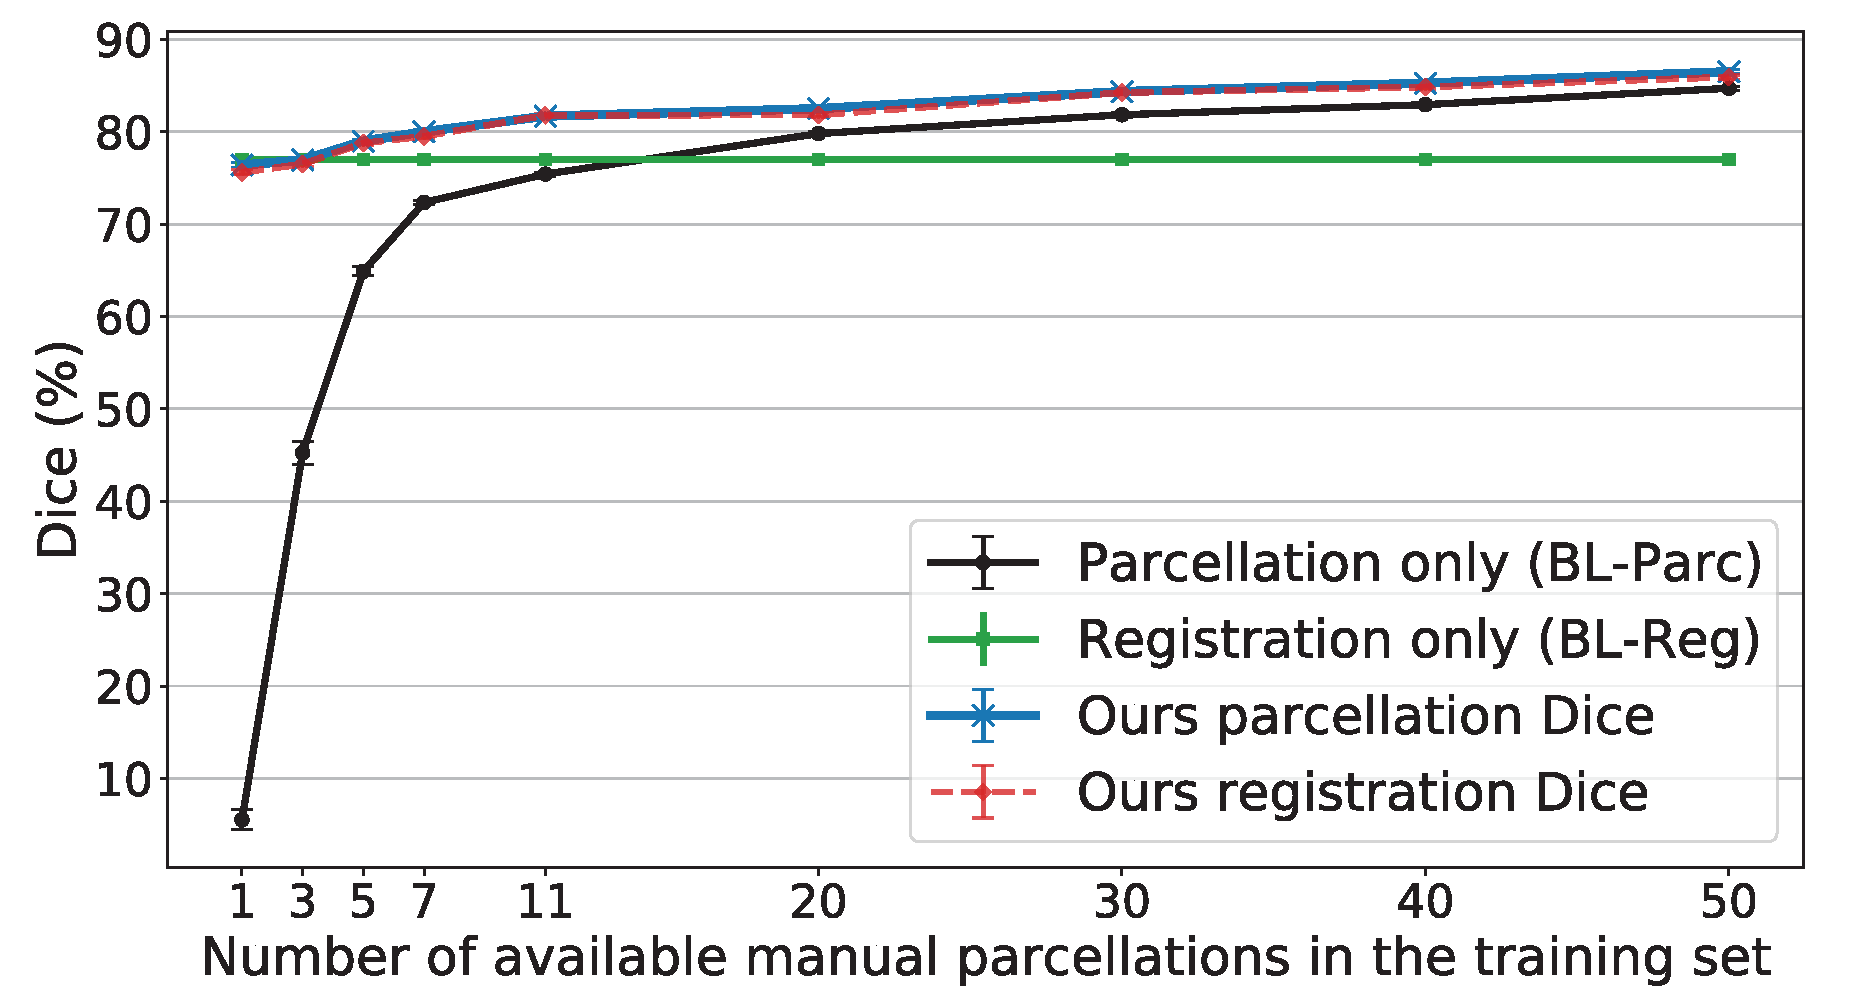
\includegraphics[width=0.7\linewidth]{figure/jrp_Figure_dice.eps}
	\caption{随机选取一定数量的人工标记的数据训练JRP-Net得到的Dice值。图中画出的是10次随机选取的平均结果和方差。} \label{fig:jrp_dice}
\end{figure}
显示了在测试集上10次实验的平均结果。可以看到,在只有atlas拥有人工标注的ROI标签的极端情况下,即11个UNC 4D atlas\cite{li2015construction},本章提出的JRP-Net方法仍然取得了不错的结果,相比独立训练的模型有很大的改进。这证明了配准任务确实为未标注的皮层表面提供反向配准的atlas的人工标记ROI图,用来扩充数据集,从而为分区任务提供了额外的半监督信息,在有些工作\cite{xu2019deepatlas}中这也叫做一种数据增强手段。反过来,可以看出即使使用预测的分区图来计算ROI分区的一致性,配准性能也能在分区任务的帮助下有所提升(当$N>3$)。同时我们还注意到,图\ref{fig:jrp_dice}中的JRP-Net的配准Dice和分区Dice的线条是高度重合的。对10次实验进行了显著性水平为0.05的配对t检验后,结果证实了配准和分区任务的Dice结果之间并没有显著性差异。这可能是因为两个任务相互引导训练,成功利用SE学习到了最优的皮层特征表达,然后两个任务特定的解码器都成功地找到了两个任务的最优解。图\ref{fig:jrp_registraionExamples}
\begin{figure}[h]
	\centering
	\includegraphics[width=\linewidth]{figure/jrp_registraionExamples.eps}
	\caption{几个典型的球面大脑皮层表面配准的例子。图中所有的方法都公平地将特征(sulc和curv)作为输入,并输出球面变形场用于配准moving surface,且图中的人工标记的ROI图只是为了验证配准性能,并没有用来预测变形场。} \label{fig:jrp_registraionExamples}
\end{figure}
展示了一些来自测试集的实际配准案例,可以看到当前可用的配准方法都无法成功地将这些皮层表面对齐好,但使用本章提出的JRP-Net($N$=50)却能得到非常好的对齐结果。这是因为当前方法的一个固有的内在缺陷,即它们只使用了特征相似性作为配准的目标函数,而本章开发的JRP-Net结合了ROI分区图相似性便可以有效地解决这个问题。

\section{讨论}
首先,对于大脑皮层分区任务,我们知道医学图像的标注工作是十分繁琐耗时的,更别提在manifold空间的大脑皮层上进行手工ROI的标记,因此可以用于训练大脑皮层分区的ROI分区金标准在实际应用情况中非常地稀少。本章提出的同时配准与分区框架正是针对这一点,在只拥有极少数的人工标记好的大脑皮层ROI分区图的前提下,利用了近几年医学图像领域中流行的半监督分割方法,即使用配准网络先生成大多数没有人工标注的皮层的伪ROI分区图,再用这些生成的伪分区图一起训练分区网络。虽然这样的伪分区图肯定不如直接用人工标注的金标准好,但是它可以极大地节省人力物力财力,而且再加上本章开发的同时与配准算法训练的策略,最终获得了非常令人满意的分区结果。总结来讲,整个实验过程最关键的地方依然在于我们仅用了极少数的手动标记数据完成了非常高质量的分区模型训练,这对大脑皮层分区任务具有十分重要的意义。

另一方面,大脑皮层配准是一个非常复杂的问题,这一章的工作中也只使用了大脑形态学几何特征来做配准。相比\ref{sec:基于三个正交球面U-Net的快速球面配准算法}的配准算法,这一章对配准问题做了一定的简化,因为本章的重点在于同时分区与配准的框架,而不是很关心具体的分区或配准的网络。因此,在大脑皮层多模态配准方面,本章的工作还存在一些局限性,这也为我们将来的工作指明了方向。即使如此,本章在基于大脑皮层形态学几何特征指导的大脑皮层褶皱的配准上取得了非常显著地巨大的提升。这个提升主要来自于分区网络得到的ROI分区图的额外的弱监督信息,这是以往的配准算法所不具有的,而且这对于以往的配准算法来说是一个固有的无法解决的问题,因为它们大多使用特定的数学模型来求解一个优化方程,因此不容易扩展地去使用额外的监督信息来驱动配准。因此,本章提出的方法可以为大脑皮层任务提供超过10\% Dice的配准效果提升,这对于大脑皮层配准具有十分重大的意义,对于整个领域来说也会有非常重要的影响。

\section{本章小结}
本章提出了JRP-Net用于皮层表面的同时配准和分区,利用了共享编码器和分区图相似性损失函数将这两个任务紧密地关联起来。通过利用两个任务之间的内在关系,本章开发的共享编码器可以有效地提取两个任务共享的更有意义的皮层高级特征,而分区图相似性损失函数则进一步地促进实现了两个任务之间的相互帮助、指导与训练。所有的实验结果,包括定量的和定性的,都表明本章提出的方法在配准和分区方面相比单独训练的配准和分区网络有很大的改进。这个改进对两个任务都具有非常重大的意义。





%%%%%%%%%%%%%%%%%%%%%%%%%%%%%%%%%%%%%%%%%%%%%%%%%%%%%%%%%%%%%%%%%%%%%%%%%%%%%%%%%%%
%% 第5章 基于球面U-Net的多中心皮层属性数据结合方法
%%%%%%%%%%%%%%%%%%%%%%%%%%%%%%%%%%%%%%%%%%%%%%%%%%%%%%%%%%%%%%%%%%%%%%%%%%%%%%%%%%%



\chapter{基于球面U-Net的多中心皮层属性数据结合方法}\label{sec:基于球面U-Net的多中心皮层属性数据结合方法}


在经过上述几章快速准确的皮层数据预处理后,我们期望获得高质量的多模态皮层属性数据。这些属性数据一般是逐个顶点的(vertex-wise)或逐个ROI的(ROI-wise)的皮层属性图,例如皮层厚度、表面积、脑沟深度、脑沟曲率、髓鞘含量和皮层扩散性等,然后研究人员就可以方便地使用任何一个中心采集的数据研究大脑发育或神经系统性疾病。然而结合多中心的数据可以显著增加数据集的样本数量,增强数据分析的统计能力,并提高结果的可信度。但是直接结合多中心的大脑皮层属性数据,例如皮层厚度,将不可避免地引入非生物学的差异,这通常是由扫描仪在成像采集协议(如视场,空间分辨率等)和扫描仪自身硬件(如制造商,磁场强度,线圈通道等)的差异所导致的。因此,结合多中心的神经影像数据要求消除这些非生物学的差异,同时还要保留生物学的差异。这已经成为多中心的神经影像数据联合分析的关键,尤其在近几年越来越多的大规模多模态神经影像研究变得越来越火热的情况下。注意本论文使用“采集中心(site)”来偶尔代替“扫描仪(scanner)”,以达到更流畅的叙述目的。

然而,目前很少有人研究关注这个问题。正如在\ref{sec:绪论}的\ref{sec:绪论_多中心皮层属性数据结合}中介绍过的相关工作,目前大多数的工具或方法只关注结构MR图像或从MR图像提取的脑体积特征的结合\cite{pomponio2020harmonization},或者DWI图像以及从DWI图像中提取的特征的结合\cite{karayumak2019retrospective},对于皮层属性数据的结合依然没有有效的方法被开发利用。唯一的通用的数据结合工具Combat\cite{fortin2018harmonization}是一种基于统计学先验知识的被广泛应用于生物学数据、成人皮层属性数据的结合方法。但是,Combat方法有三个局限性。(1)它是一个ROI层面的线性模型,因此在婴儿数据上可能无法适应多中心数据之间的复杂的非线性映射;(2)它的优化过程假设模型参数都遵循一个特定的先验分布,这在皮层属性结合的很多场景下可能并不成立;(3)Combat是将两个中心的数据合并成一个中心而设计的,不适用于将一个低质量的数据集映射到另一个可靠的中心的高质量数据集上。针对这些局限性,本章提出了一种新型的基于深度学习的方法来结合多中心的大脑形态学属性。另外,本章开发的方法具有很强的学习能力,可以学习不同中心数据之间复杂的点对点的映射关系,因此比基于统计学的Combat工具具有更强的泛化能力。

近几年虽然没有明确地开发出用于皮层属性数据结合的方法,但最近的一些深度学习技术\cite{zhao2019spherical_ipmi,zhu2017unpaired}可以被修改后用于解决这个问题。首先,球面U-Net结构\ref{sec:球面U-Net}提供了一个有效的1-ring卷积核,将传统的CNN扩展到了具有固定球形拓扑属性的大脑皮层表面。在前几章中,它已经在皮层表面分区、配准、皮层发育属性预测等任务上取得了非常好的效果,实现了目前最先进的基于深度学习的皮层表面数据的处理与分析,因此我们考虑可以将它作为中心到中心的皮层表面属性图转换的生成器。其次,由于大多数神经影像学研究没有跨中心的配对数据,流行的图像生成技术CycleGAN\cite{zhu2017unpaired}可以被利用来生成无配对的皮层表面数据的迁移。因此,在借助球面U-Net的帮助下,本论文提出将传统的CycleGAN扩展到皮层表面上,称为Surface-to-Surface GAN,简称S2SGAN。具体地,我们把从中心$X$到中心$Y$的数据映射建模为一个球形表面到另一个球形表面的数据迁移任务。数据结合的初步目标就是学习一个映射$G_X:X\rightarrow Y$,使$G_X(X)$的分布与$Y$的分布无法区分。由于这个映射是高度低约束的,而数据结合的第二个目标是要保留生物学差异,因此我们再利用逆映射$G_Y: Y\rightarrow X$和循环一致性损失来强制要求$G_Y(G_X(X))\approx X$(反之亦然)。此外,我们还加入了相关系数损失,以更好地保证原始皮层表面属性图和生成的皮层表面属性图之间的结构一致性。	
	

\section{多中心皮层属性数据结合的网络结构}

\subsection{损失函数设计}
如图\ref{fig:s2sgan_architecture}(a)所示,假设我们有两个皮层表面数据集,从两个不同的扫描仪获得,即扫描仪$X$和扫描仪$Y$。数据结合的目标是学习皮层表面属性图(例如皮层厚度)的跨中心映射函数$G_X$和$G_Y$,它们分别完成映射$X\rightarrow Y$和$Y\rightarrow X$。此外,判别器$D_X$用于区分真实的和生成的$X$扫描仪的表面属性图,判别器$D_Y$用于$Y$扫描仪的属性图真伪判别。所有的映射和判别函数都可以用我们在\ref{sec:基于球面U-Net的皮层分区与属性预测}中开发的球面神经网络的基本操作的组合来近似。因此整个模型的优化目标包括三种类型的损失函数:(1)对抗性损失,用于将生成的球面属性图的分布与目标中心的分布相匹配;(2)循环一致性损失,用于防止生成器生成与输入无关的属性图;(3)相关系数损失,用于约束原始属性图和生成的属性图之间的结构一致性。
	
\subsubsection{对抗性损失函数}
本章提出的方法首先对两个映射函数$G_X:X\rightarrow Y$和$G_Y:Y\rightarrow X$应用对抗性损失。具体来讲,对于映射函数$G_X$和它的判别器$D_Y$,目标函数定义为:
\begin{equation}\label{eq:5-1}
	{{\cal L}_{GAN}}({G_X},{D_Y}) = {E_{x\sim{p_{data}}(X)}}[{(1 - {D_Y}({G_X}(x)))^{\rm{2}}}] + {E_{y\sim{p_{data}}(Y)}}[{D_Y}{(y)^2}],
\end{equation}
其中$x\sim p_{data}(X)$和$y\sim p_{data}(Y)$代表$X$和$Y$的数据分布。$G_X$的目的是生成与$Y$中心的真实皮层表面属性图尽量接近的假属性图,即$G_X(x)$,而$D_Y$则是用来区分生成的假属性图和$Y$中心的真实皮层属性图。因此,这个极小极大化(minimax)博弈游戏的优化过程可以写成:$mi{n_{{G_X}}}ma{x_{{D_Y}}}{{\cal L}_{GAN}}({G_{\rm{X}}},{D_Y})$。同时,我们对$G_Y$和$D_X$也采用了类似的对抗性损失与训练策略。

\begin{figure}[t]
	\centering
	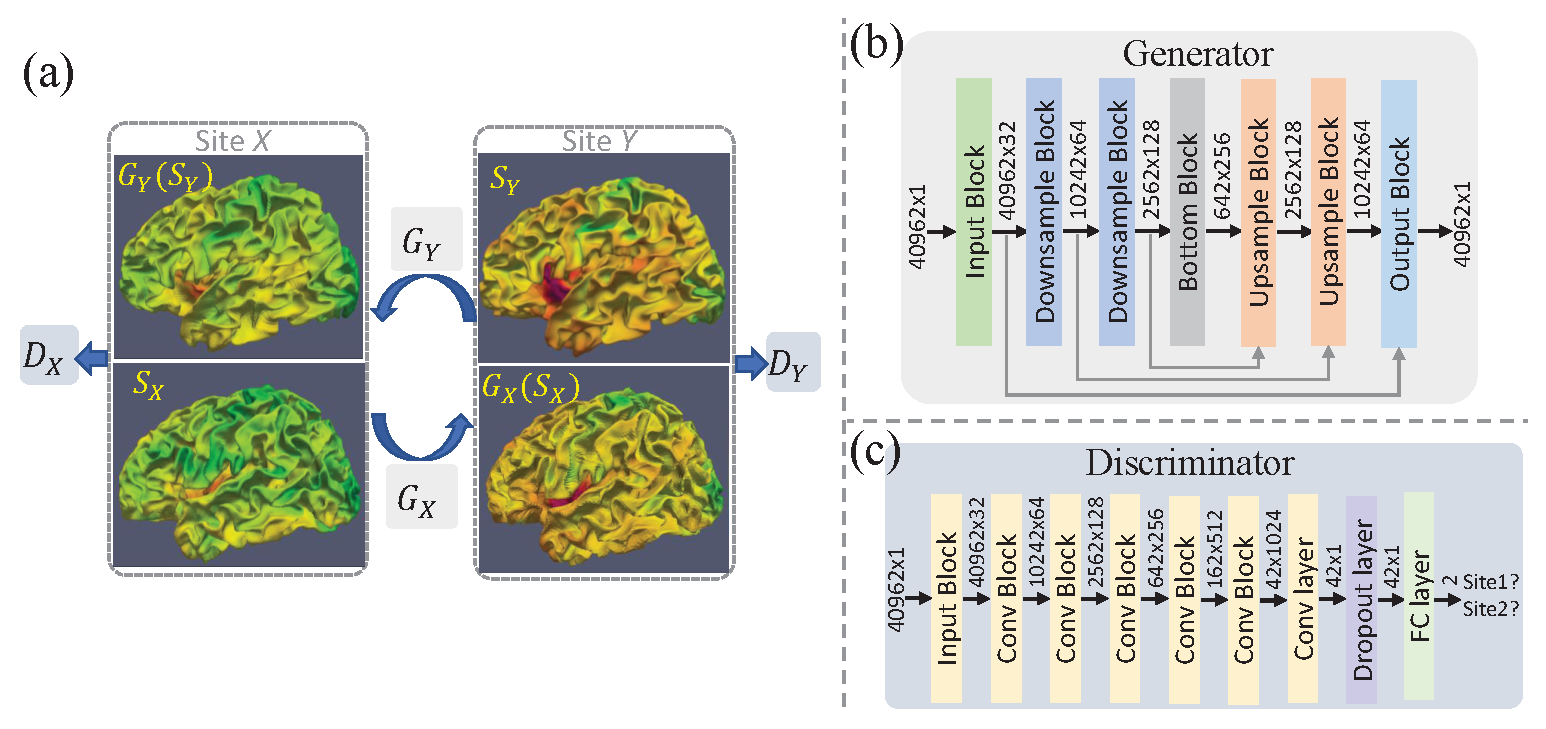
\includegraphics[width=\linewidth]{figure/s2sgan_architecture.eps}
	\caption{用于多中心皮层属性数据结合的S2SGAN网络结构。(a)两个生成器($G_X$和$G_Y$)分别学习皮层表面属性图(例如图里展示的皮层厚度图)的跨中心映射关系。两个鉴别器($D_X$和$D_Y$)用于区分生成的表面属性图和真实的表面属性图的真伪性。(b)在生成器中,每个单元(block)的操作包含重复的1-ring Conv+BN+ReLU,输入大小和输出大小标记在了每一个单元的前后,每个下采样单元还要多一个球面池化层,上采样单元多一个球面转置卷积层,用来处理跳跃式连接串联的特征图(灰色箭头所指示的)。(c)在判别器中,除了输入单元没有池化层以外,每个单元都包含1-ring Conv+BN+ReLU+Pooling。}\label{fig:s2sgan_architecture} 
\end{figure} 
	
\subsubsection{循环一致性损失函数}
因为对抗性损失只是保证了生成的数据与目标中心的数据无法区分,也就是说生成了一个假的目标中心球面数据,但是却无法保证生成的图是有意义的,所以生成的这个球面可能与原始输入的球面属性图已经完全没有任何关系了。为了保证生成的球面属性图与原始的球面属性图是相关的,我们额外加入了循环一致性损失\cite{zhu2017unpaired}。它被定义为原始球面图和重建的球面图之间的差异,即:
\begin{equation}
	   	{{\cal L}_{cyc}}({G_X},{G_Y}) = {E_{x\sim{p_{data}}(X)}}[{\left\| {{G_Y}({G_X}(x)) - x} \right\|_1}] + {E_{y\sim{p_{data}}(Y)}}[{\left\| {{G_X}({G_Y}(y)) - y} \right\|_1}]. 
\end{equation}

\subsubsection{相关系数损失函数}
在映射函数中保留皮层表面属性图的局部结构信息是至关重要的。为了进一步减少原图和生成的目标图之间由于间接的循环一致性损失造成的模糊性,我们采用相关系数损失来约束输入和输出的表面图之间的结构一致性:
\begin{equation}
	{{\cal L}_{cc}}({G_X},{G_Y}) =  - {E_{x\sim{p_{data}}(X)}}[\frac{{{\mathop{\rm cov}} ({G_X}(x),x)}}{{{\sigma _{{G_X}(x)}}{\sigma _x}}}] - {E_{y\sim{p_{data}}(Y)}}[\frac{{{\mathop{\rm cov}} ({G_Y}(y),y)}}{{{\sigma _{{G_Y}(y)}}{\sigma _y}}}],
\end{equation}
其中$cov$表示协方差,$\sigma$表示标准差。
	
\subsubsection{可选的配对数据损失函数}
在本章提出的方法中,我们不需要任何来自不同中心的配对数据进行训练,因为这些数据通常是很难获得的。但是,如果我们有配对数据,便可以增加一个额外的配对损失来直接约束生成的球面图和金标准属性图之间的vertex-wise的相似度:
\begin{equation}
	{{\cal L}_{pair}}({G_X},{G_Y}) = {E_{x\sim{p_{data}}(X)}}[{\left\| {{G_X}(x) - gt(x)} \right\|_1}] + {E_{y\sim{p_{data}}(Y)}}[{\left\| {{G_Y}(y) - gt(y)} \right\|_1}],
\end{equation}
其中$gt(x)$,$gt(y)$代表配对数据集中$x$和$y$的金标准。
	
\subsubsection{完整的目标函数} 
最后,训练S2SGAN模型的完整的目标函数可以写成:
\begin{equation}
\begin{split}
    {\cal L}({G_X},{G_Y},{D_X},{D_Y}){\rm{ = }} & {{\cal L}_{GAN}}({G_X},{D_Y}) + {{\cal L}_{GAN}}({G_Y},{D_X}) + \alpha {{\cal L}_{cyc}}({G_X},{G_Y})  \\
    & +\beta {{\cal L}_{cc}}({G_X},{G_Y}) + \lambda {{\cal L}_{pair}}({G_X},{G_Y}),
\end{split}
\end{equation}
其中$\alpha$,$\beta$和$\lambda$是每一个损失函数项的权重。因为最后一项是可选的配对数据损失函数,所以当没有配对数据时,完整的目标函数中也就没有最后一个损失项了。
	
\subsection{网络结构}
这个工作依然利用皮层表面的球形拓扑结构并使用\ref{sec:球面U-Net}中的球面U-Net结构作为我们的生成网络\ref{sec:球面U-Net}。球面U-Net首先利用1-ring卷积核在恒定的重采样的正二十面体离散化球面上进行卷积、池化和上采样操作,将卷积、池化和上采样操作扩展到了球面空间,然后利用相应的球面操作搭建了U-Net。本章工作对原始的\ref{sec:球面U-Net}中的球面U-Net进行了修改,把分辨率级别和通道数做了相应的轻量化,减半了特征通道数并且只保留了第7级到第4级球面分形体上的4个分辨率级别,其中前3个分辨率依然使用跳跃式连接进行串联,具体的结构可以参见\ref{fig:s2sgan_architecture}(b)。对于判别器网络,我们将VGG\cite{simonyan2014very}网络,一个用于自然图像分类的优秀的CNN结构,扩展到了球面。它由7个1-ring球面卷积层、5个球面池化层、一个概率为0.2的dropout层和1个全连接层组成,如图\ref{fig:s2sgan_architecture}(c)所示。另外,所有的1-ring球面卷积层后面都接有一个批量归一化层(BN)和一个斜率为0.2的leakyReLU层。

	

\section{实验与结果}

\subsection{合成的配对数据的实验与结果}\label{sec:Synthetic}
为了更好地评估本章方法在不同中心的皮层属性数据结合上的性能,我们合成了一个配对的数据集,用来模拟从不同分辨率扫描的图像重建的皮层表面,这是一个典型的经常发生在实际应用中的数据结合场景。具体来讲,这个实验使用了和\ref{sec:基于球面神经网络的大脑皮层同时分区与配准}中同样的BCP\cite{howell2019unc}婴儿数据集,共有来自183名婴儿的360个MRI扫描数据,年龄从0到2岁,我们把这组数据的扫描中心命名为$X$。T1w和T2w图像的分辨率均为$0.8\times 0.8\times 0.8mm^3$。我们将中心$X$中的所有T1w和T2w图像重新采样到了$1\times 1\times 1mm^3$,便形成了另一个数据集,称作中心$Y$。所有的MR图像都使用了婴儿专用的计算pipeline(iBEAT V2.0 Cloud, http://www.ibeat.cloud/)进行了处理。然后所有的皮层表面都被映射到了球面空间,非线性配准好并进一步重新采样到第7级正二十面体分形球面上。

在这个实验中,对于没有配对数据的S2SGAN模型,我们设置$\alpha$为15,$\beta$为1,$\lambda$为0;对于有配对数据的S2SGAN模型,设置$\alpha$为15,$\beta$为1,$\lambda$为100。本实验使用了Adam优化器训练这两个模型,在前20个epoch中以0.0001的初始学习率交替学习$G$和$D$,在接下来的180个epoch中线性地将学习率降低至0,使用了70\%的数据作为训练集,剩余的30\%作为测试集,并采用了分层采样的方法确保同一个个体的不同时间点的数据都在同一个集合中,并且也确保了每个集合中的年龄分布尽可能地相似。本实验采用平均绝对误差(MAE)和峰值信噪比(Peak signal-to-noise ratio, PSNR)这两个广泛使用的相似性指标来定量地评估生成结果的好坏。

本实验训练的S2SGAN模型把低质量中心$Y$的皮层厚度数据映射到了高质量中心$X$上,从而完成了在中心$X$的域内结合了所有的皮层厚度数据。平均而言,默认S2SGAN模型获得的MAE结果为0.093$\pm$0.011mm,PSNR为31.48$\pm$1.12(标准差是基于所有皮层结果的)。使用了配对数据并利用配对数据损失函数来训练的S2SGAN(paired)模型达到了MAE 0.082$\pm$0.018mm,PSNR 33.09$\pm$1.73的结果,这个代表了S2SGAN所能达到的最佳效果。相比之下,使用Combat的官方代码,以年龄和性别作为统计协变量,获得的结果为MAE 0.124$\pm$0.014mm和PSNR 29.00$\pm$1.02。总的来说,本章开发的S2SGAN在MAE和PSNR方面都实现了比Combat更好的性能,并且也产生了与S2SGAN(paired)更接近的结果。图\ref{fig:s2sgan_paired_result}
\begin{figure}[h]
	\centering
	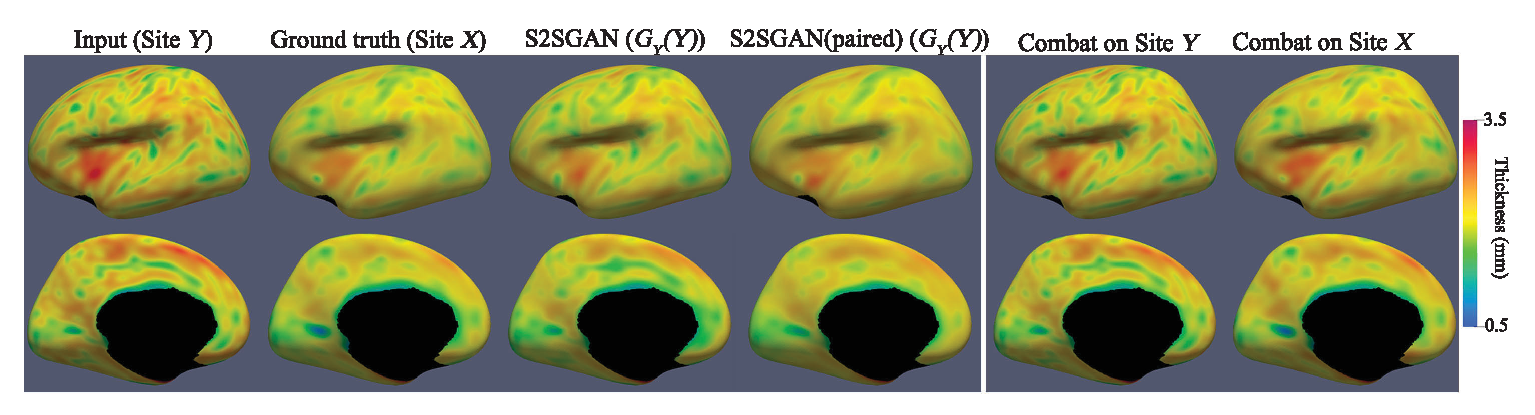
\includegraphics[width=\linewidth]{figure/s2sgan_paired_result.eps}
	\caption{在一个测试对象上使用不同数据结合方法得到的结果比较。前四列是S2SGAN模型的结果。最后两列是Combat的结果。注意Combat将两个中心结合为一个中间中心,因此最优的结果应该是在最后两列生成两个非常一致的皮层表面。}\label{fig:s2sgan_paired_result} 
\end{figure} 
直观地显示了不同方法在一个随机选取的测试对象上的数据结合结果的定量比较。


\subsection{真实的皮层表面数据结合实验与结果}
为了证明本章的方法在实际的多中心皮层表面数据结合上的优势,本小节实验采用了两个真正的纵向长期婴儿数据集。这两个数据集拥有匹配的人口统计信息,即年龄范围相似,年龄分布也相似。其中中心$X$依然还是在\ref{sec:Synthetic}中使用的$X$中心的数据,而中心$Y$是来自Multi-visit Advanced Pediatric (MAP)数据库的50个婴儿的251个不同时间点的MRI扫描数据。MAP数据集使用了一台Siemens Trio扫描仪以$1\times 1\times 1mm^3$的分辨率采集得到。因此这两个数据集之间不可避免地会存在扫描仪影响,这个实验的目的即是利用本章提出的S2SGAN模型学习并消除这种扫描仪影响,同时还要保留相关的生物学差异。我们使用了和\ref{sec:Synthetic}中相同的预处理方式以及同样的超参数训练得到了最终的S2SGAN模型。




\subsubsection{验证是否消除了扫描仪影响}
因为真实采集的数据并没有配对的数据,即一个受试者一般只在一个中心的一台扫描仪上进行数据采集,所以我们无法知道这些受试者在另一台扫描仪上采集得到的数据是什么样的。也就是说,无配对数据是没有金标准来衡量一个生成结果的好坏的。因此,本小节使用了与以往方法\cite{karayumak2019retrospective}相同的评价指标来执行基于ROI的分析,验证是否去除了扫描仪效应。理论上,在年龄分布相匹配的情况下,数据结合后,映射到另一个中心的数据应该达到与目标中心数据相一致的平均ROI皮层厚度值。图\ref{fig:s2sgan_roi_bar_realA_realB_fakeA}
\begin{figure}[h]
\centering
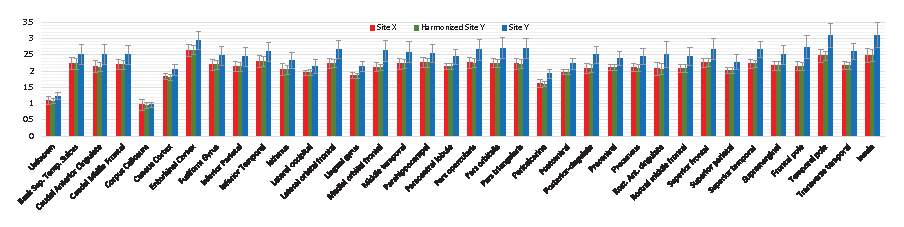
\includegraphics[width=\linewidth]{figure/s2sgan_roi_bar_realA_realB_fakeA.eps}
\caption{数据结合前后不同采集中心的大脑皮层厚度数据分布。横轴为每个ROI的名称,纵轴为ROI的平均皮层厚度值。}\label{fig:s2sgan_roi_bar_realA_realB_fakeA} 
\end{figure}
显示了中心$X$、中心$Y$和结合后中心$Y$的36个ROI的平均厚度值。可以看到ROI厚度的统计显著性差异在结合前是存在的,而在结合后都被成功地消除了。另外,我们还使用了Fortin等人在Combat\cite{fortin2018harmonization}工作中采用的评价方法,即对site $X$ + site $Y$ + 结合后的$Y$的vertex-wise的皮层厚度数据使用主成分分析法(Principal component analysis, PCA)进行无监督降维。然后把投影到前两维的主成分值画在了图\ref{fig:s2sgan_pca}
\begin{figure}[h]
\centering
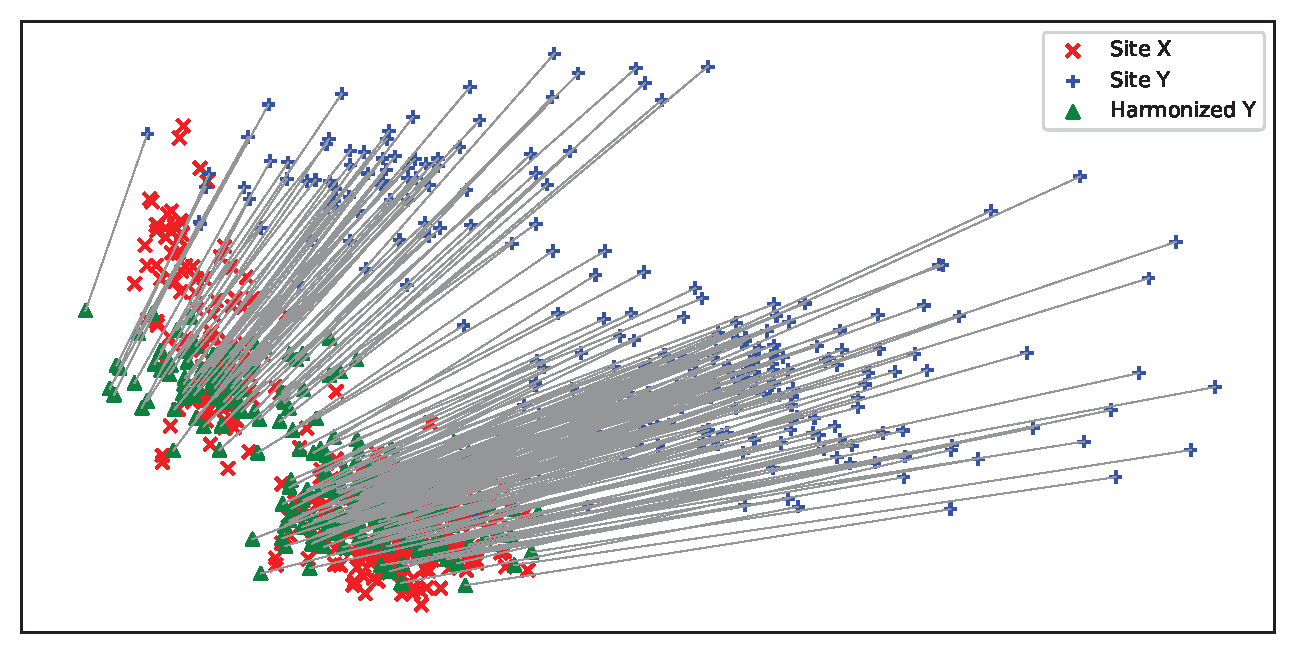
\includegraphics[width=\linewidth]{figure/s2sgan_pca.eps}
\caption{采用PCA对中心$X$+中心$Y$+映射到$X$中心的$Y$数据进行降维的结果,其中$x$轴为第一主成分,$y$轴为第二主成分。灰色的线代表映射前后同一个皮层数据的对应关系。}\label{fig:s2sgan_pca} 
\end{figure} 
中。图\ref{fig:s2sgan_boxplot}
\begin{figure}[h]
\centering
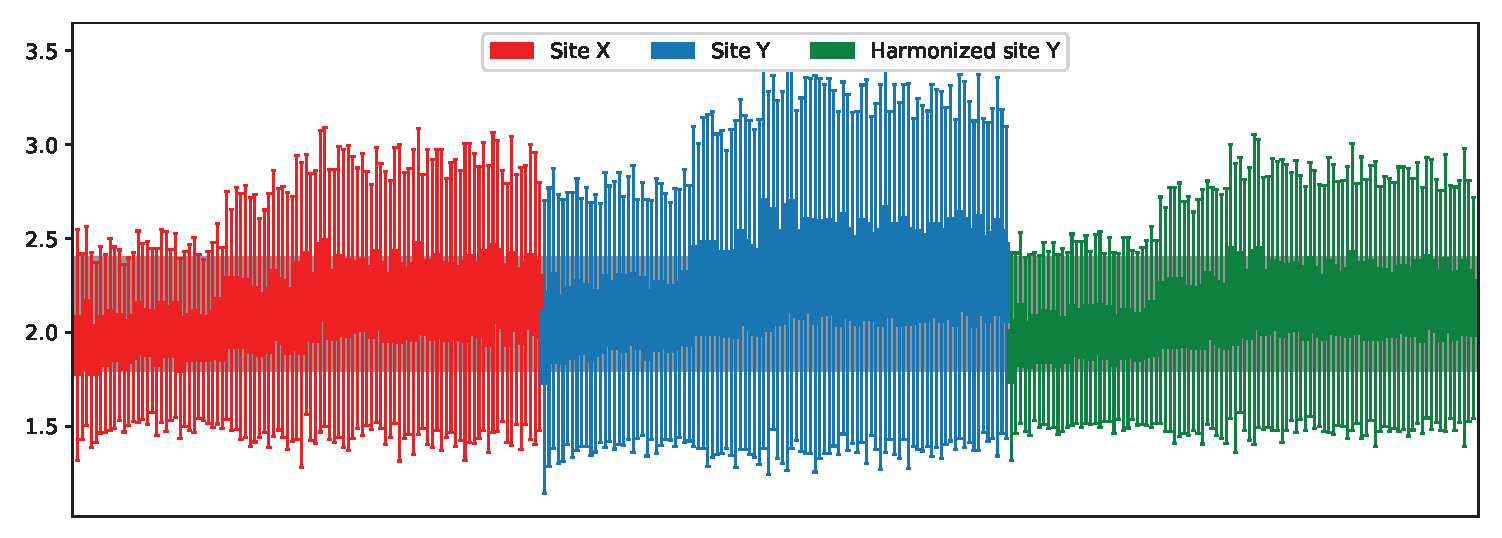
\includegraphics[width=\textwidth]{figure/s2sgan_boxplot.eps}
\caption{不同中心的100个样本的vertex-wise的皮层厚度箱形图。每一个箱形图代表一个样本。每一个中心都有100个分层采样的样本并在中心内的按年龄由小到大地排序。}\label{fig:s2sgan_boxplot} 
\end{figure} 
显示了分别来自中心$X$、中心$Y$和结合后的$Y$的100个样本的vertex-wise的皮层厚度箱形图。在这个图中,我们按分层采样的方法随机选择了100个样本的数据并按年龄由小到大地进行排列。综上,所有结果都验证了本章提出的方法不仅实现了将源中心的数据成功结合到目标中心,还同时很好地保留了个体差异。

\subsubsection{验证是否保留了组间差异}
这一小节采用了Karayumak等人\cite{karayumak2019retrospective}文中也使用的Cohen's d指标来评价不同年龄组之间差异的保留情况。Cohen's d的定义是:
\begin{equation}
 {d_{ij}} = \frac{1}{{{N_r}}}\sum\limits_r {\left| {({M_{ir}} - {M_{jr}})/\sqrt {\frac{{({n_i} - 1)s_{ir}^2 + ({n_j} - 1)s_{jr}^2}}{{{n_i} + {n_j} - 2}}} } \right|},
\end{equation}
其中$i$和$j$代表两个不同的组,$r$代表每个ROI的特征,$N_r$是ROI的数量,$M$是平均皮层厚度值,$s$是标准差,$n$是每个组内样本的数量。因此,Cohen's d不受数据大小的影响,一般在0.1~2.0之间,与组间的差异大小成正比。然后我们将所有的数据分别以45天、135天、225天、315天、450天的年龄为界分为6组,再分别计算其中任意两组的Cohen's d,最后算出数据结合前后所有组之间的Coehen's d的平均绝对偏差:
\begin{equation}
     \Delta d = \frac{1}{{{N_g}({N_g} - 1)}}\sum\limits_{i = 1}^{{N_g}} {\sum\limits_{j \ne i}^{{N_g}} {\left| {d_{ij}^{before} - d_{ij}^{after}} \right|} },
\end{equation}
其中$N_g$是组的数量,$d_{ij}^{before}$和$d_{ij}^{after}$分别代表了数据结合前后的Cohen's d。因此,较小的$\Delta d$一般代表较好的组间差异保留。为了与Combat方法进行比较,我们使用了Combat的官方代码,把年龄作为协变量,得到的$\Delta d$结果为0.2069$\pm$0.1467,而S2SGAN获得了$\Delta d=$0.0683$\pm$0.0520的结果。由此我们可以得出结论,本章提出的方法在将多中心的数据结合后可以更好地保留不同数据组之间的差异性。特别地,在这个实验中,更好地保留了不同年龄组之间的皮层厚度数据的差异性,对于后续的联合分析大脑皮层属性发育与疾病的关系非常有帮助。

\subsubsection{验证是否保留了个体差异}
同样地因为没有配对数据,本小节使用了别人曾经使用过的证实为有效的指标来衡量数据结合前后个体差异有没有被保留。像Huynh等人\cite{huynh2019multi}的工作一样,本小节也使用ROI特征值来计算任意两个样本之间的欧式距离,从而形成一个距离矩阵,表示为${\bf{E}}_{ij}^{n \times n}{\rm{ = }}{\left\| {{F_i} - {F_j}} \right\|_{\rm{2}}}$,其中$n$是样本个数,$F$是皮层厚度特征向量。与Huynh等人\cite{huynh2019multi}唯一不同的是我们使用的是ROI-wise的皮层厚度平均值,而不是subject-wise的皮层厚度中位值来计算距离矩阵,因为我们的目的是估计在数据结合前后每两个样本之间的距离的相对保留情况。因此,我们随后计算了数据结合前后两个距离矩阵的相关性$Cor$。然后同样与使用了年龄和性别作为协变量的Combat方法进行了比较。最后结果显示,本章开发的S2SGAN获得的$Cor$为0.9766,而Combat的$Cor$为0.9606。较高的$Cor$验证了本章提出的方法在将多中心的数据结合后更好地保留了个体差异。最后,图\ref{fig:s2sgan_examples}
\begin{figure}[h]
	\centering
	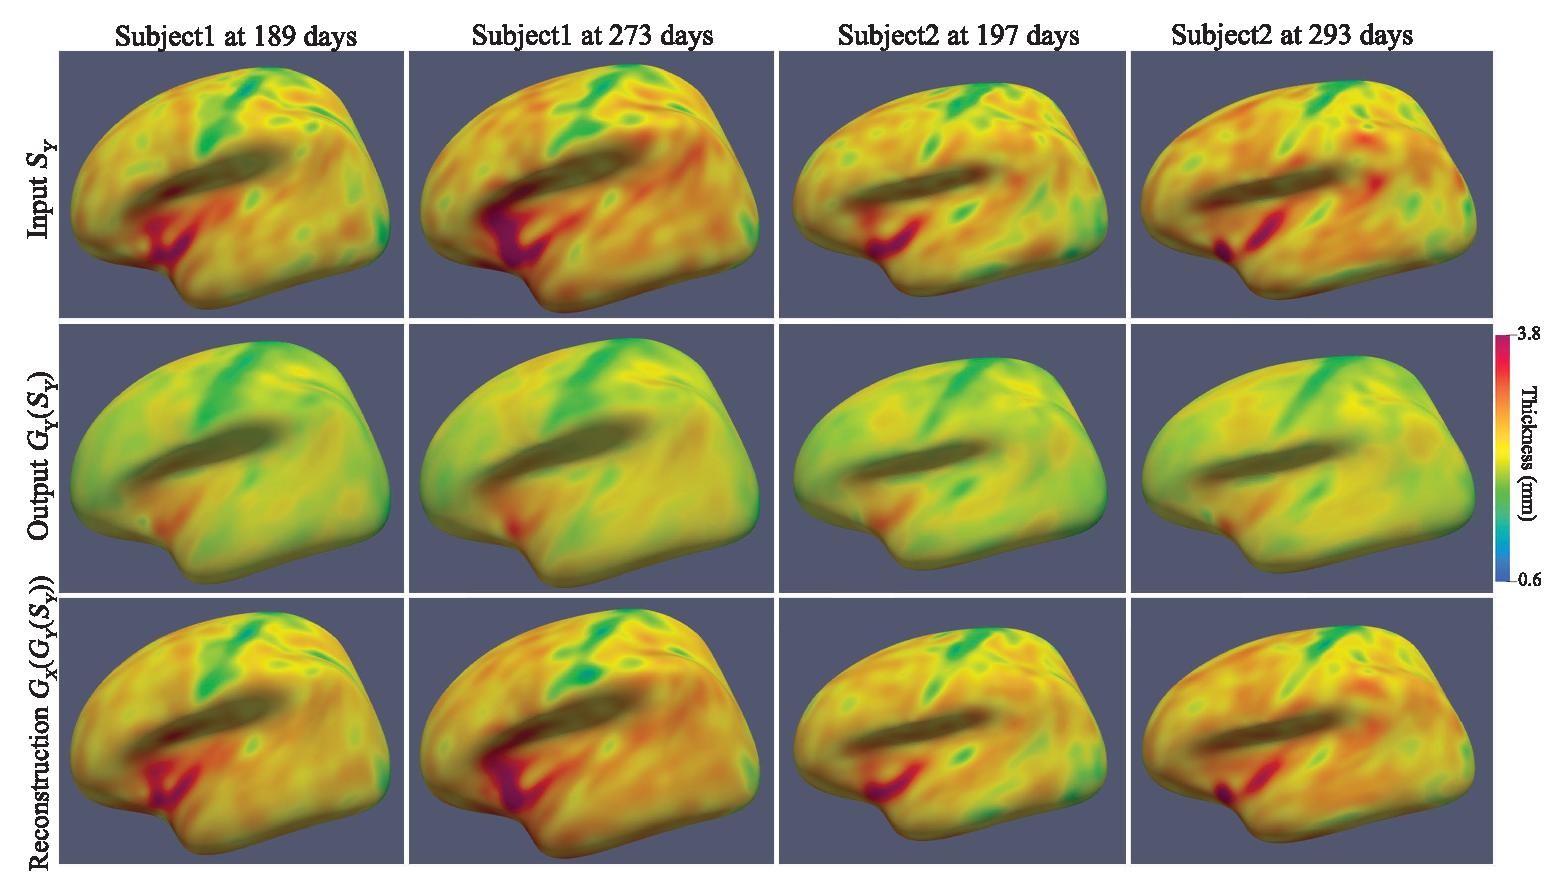
\includegraphics[width=\linewidth]{figure/s2sgan_examples.eps}
	\caption{S2SGAN对两个年龄相匹配的测试样本进行皮层厚度结合的可视化结果。}\label{fig:s2sgan_examples}
\end{figure}
显示了两个年龄相匹配的测试样本的皮层厚度结合结果。我们可以看到无论是个体还是年龄组之间的差异都得到了很好的保留。

需要指出,本章提出的方法适用于任意两个中心采集到的神经影像数据的结合,但是对于每两个中心数据的相互结合,我们都需要重新训练或者微调模型。这在一些小规模的神经影像数据处理与研究计划中,对于比较少量的中心或扫描仪个数来说,还可以接受,但是很明显如果中心数目变多,我们需要花费的时间精力以及存储计算资源都会大幅增加。这是本章方法的一个局限性所在,也是我们未来的研究方向之一。解决这个问题的一个可能的方法便是让网络中的生成器可以自由选择生成的目标中心,由此来设计一个多中心的数据生成与结合网络。我们将在\ref{sec:总结与展望}的工作展望中对此进行详细叙述。

\section{本章小结}
这一章提出了一种基于球面U-Net和CycleGAN的新型球面神经网络用于皮层属性数据结合,称作S2SGAN网络。利用深度学习的强大能力,S2SGAN成功地学习了从一个中心到另一个中心皮层属性数据的复杂映射关系。S2SGAN方法已经在婴儿大脑MRI的合成配对数据和真实的非配对数据上得到了广泛的验证。定量的和定性的结果都表明了其消除不同中心数据之间的扫描仪差异的优越能力,同时还能很好地保留了个体与组间差异。





%%%%%%%%%%%%%%%%%%%%%%%%%%%%%%%%%%%%%%%%%%%%%%%%%%%%%%%%%%%%%%%%%%%%%%%%%%%%%%%%%%%
%% 第6章 总结与展望
%%%%%%%%%%%%%%%%%%%%%%%%%%%%%%%%%%%%%%%%%%%%%%%%%%%%%%%%%%%%%%%%%%%%%%%%%%%%%%%%%%%




\chapter{总结与展望}\label{sec:总结与展望}

\section{论文工作总结}
随着MRI这个非侵入式的无创生物医学成像技术的问世与发展,采集大脑MR图像、观察并研究大脑发育与病变变得越来越容易。这促进了最近十几年来的大规模神经影像学研究,对婴幼儿早期大脑发育的研究、神经退行性疾病的临床医学诊断等都具有非常重大的意义,让我们不断加深了对大脑发育与大脑神经系统性疾病的理解。然而越来越多的数据对大脑MR图像处理pipeline提出了更高的要求,当前可以使用的很多传统算法已经适应不了大规模多中心的MRI数据处理与分析的场景。其中基于脑体积的分析已经开发了很多基于深度学习的算法来提高其速度与精度,解决了很多大脑MR图像处理中的难题,然而基于脑皮层的数据处理与分析大多还是基于传统的手工提取特征和机器学习的方法,在很多应用上已经满足不了大规模神经影像数据处理所要求的速度与准确度。这对基于脑皮层的数据处理与分析是一个非常有挑战性的工作。因为大脑皮层是manifold空间上的不规则的结构并且每个个体之间存在着巨大的差异,在我们的工作之前仍然没有有效的改善整个脑皮层数据处理与分析的工作出现。

本论文的主要目的便是针对当前脑皮层数据处理与分析pipeline中存在的问题进行改进,利用深度学习方法从本质上改变整个pipeline的处理思路与流程,极大地加快了数据处理流程的同时也获得了比当前方法更准确的结果。本论文的出发点是如何有效地将深度学习方法扩展到大脑皮层表面上,因此借助球面皮层形式的规则性,开发了基于正二十面体离散化球面的1-ring卷积核,并重点围绕基于1-ring卷积核的球面深层神经网络及其在大脑皮层上的应用展开,深入研究并完成了四个基本而又关键的大脑皮层数据处理与分析中的任务,即分区、配准、发育建模与预测、多中心数据结合。总地来说,论文的主要创新点和贡献包括以下几点:

\textbf{一、基于球面U-Net的皮层分区与属性预测。}本论文首先利用大脑皮层固有的球形拓扑结构将大脑皮层映射到标准球面空间,然后再利用重采样后的大脑皮层表面的一致的正二十面体离散化球面结构,提出了一种新型的直观的自然的球面卷积滤波器,即1-ring卷积核。1-ring卷积核的定义与正二十面体的膨胀和收缩过程一致,其中的每个顶点在每次迭代过程中都会在其邻域中传播或聚合信息,因此能够通过多层次的网络结构有效地学习球面数据的特征并为所学的特征提供可靠的可解释性。基于这个新的球面卷积滤波器,我们开发了球面空间的球面卷积、池化和转置卷积,以及其升级版本可变形卷积与池化等操作。据此,本论文将流行的U-Net结构\cite{ronneberger2015u}从图像领域扩展到球面领域,搭建了球面U-Net结构及其升级版本球面可变形U-Net(SDU-Net)。

然后在两个具有挑战性的大脑皮层数据分析任务上验证了球面U-Net结构的有效性,即大脑皮层分区与皮层属性发育预测。这两个任务都具有重要的神经科学研究和临床诊断的意义,并且目前都受限于复杂耗时的人工特征的设计与提取,以及繁重的机器学习分类器或回归器的计算负担。这是因为它们都是vertex-wise的密集分类或回归问题,需要学习并预测复杂的非线性的皮层特征到vertex-wise的分区标签或顶点属性值的映射。在这两个任务中,本论文提出的球面U-Net与目前最好的算法相比,取得了更好的性能,不管是定量还是定性的结果,不管在精度上还是计算效率上,都展示了目前领域内最好的结果。这表明本论文提出的球面U-Net是一个与任务和特征无关的通用鲁棒的深度学习模型,在不同的任务中都能够自动学习到针对不同任务的有用的特征。

\textbf{二、针对大脑皮层表面配准,本论文提出了基于三个正交球面U-Net的快速球面配准算法。}皮层表面配准是基于皮层表面的神经影像分析的一个重要步骤和先决条件。它将不同个体和时间点的皮层表面对齐,以建立横向跨个体和纵向跨时间的皮层对应关系,从而方便后续的比较分析,比如群体之间的横向比较或时间上的纵向发育研究。目前的大脑皮层表面配准算法虽然取得了不错的性能,但这些方法有两大局限性:(1)不能够灵活地扩展到多模态的皮层特征。因为复杂的皮层区域与微观结构、功能区域高度相关,基于多模态皮层特征的配准才可以实现更有意义的跨个体和年龄的配准;(2)速度慢,耗时长。现有的方法通常被设计为优化每对皮层球面之间的目标函数问题,这在计算上是非常低效的,因此在处理大规模神经影像数据时,计算成本的增加越来越成为后续分析的一个阻碍。

为了解决这些问题,本论文提出了一个基于学习的皮层表面配准框架,称为快速球面配准(S3Reg)算法。首先,为了使用多模态皮层特征来进行配准,S3Reg采用了端到端的无监督学习模式,从而在输入特征和输出相似度指标的选择上提供了很大的灵活性;其次,为了加快配准过程,S3Reg的目标是从整个数据集中学习一个全局配准函数来配准任意一对球面数据,从而得到一个简化但高效的单一配准模型,可以快速地得到任意一对新的球面数据的球面变形场。本论文使用了三个正交球面U-Net来对这个配准模型进行建模,并使用由6个“缩放和平方”层组成的球面变换层来移动球面。因为网络中的所有层都是定义良好的且可微分的,因此可以通过反向传播梯度有效地学习网络参数。本论文在基于图谱的配准任务中使用了成人和婴儿数据集进行了配准实验,与目前最好的配准算法相比,S3Reg获得了相当不错的大脑皮层配准精度,但同时要运行地快得多,配准一对球面数据的时间不到10秒,而以往最快的Spherical Demons算法需要大约1分钟。这使得本论文提出的方法会成为大规模神经影像数据配准的首选,对整个基于脑皮层的数据处理与分析pipeline的速度提升具有非常重要的意义。

\textbf{三、用于同时皮层配准与分区的新型深度球面网络模型。}虽然上面两个工作在各自的任务中都取得了非常好的效果,但是也可以看出大脑皮层表面配准和分区一直以来都是作为两个任务分开单独进行的。传统上,一般都是先进行皮层表面配准再使用配准后的球面特征进行皮层分区,但是这样明显忽略了这两个密切相关的任务之间的内在联系。根本上讲,这两个任务都依赖于有意义的皮层特征的学习,所以它们可以通过学习共享的皮层特征来同时优化它们的网络参数。

为此,本论文首次研究探讨了基于球面神经网络的同时大脑皮层配准和分区的想法。本论文提出的同时配准与分区网络(JRP-Net)利用了这两个任务之间的内在固有联系,在方法上提出了两个主要的创新点,即共享编码器和新的ROI分区图相似性损失函数。它们都以合理的方式提升了这两个任务的性能。首先,共享编码器利用了这两个任务之间的内在密切关系学习了两个任务的共同特征。然后,JRP-Net分别为配准和分区任务训练了两个特定的任务解码器,并进一步利用这两个任务之间的明确联系,整合进ROI分区图相似性损失函数,强制要求预测的ROI与固定的人工标记的ROI相匹配,从而为配准任务提供额外的监督信息。反过来,分区网络训练也受益于配准任务,因为将一个带有手工标记ROI的球面配准到另一个没有手工标注的球面后,就为分区任务提供了大量额外的训练数据。因此,与单独训练的网络相比,这两个任务可以相互指导训练,相互提升对方的性能。这种互相帮助特别是在只有少数手动标记的数据可用时,对于分区和配准任务都有着巨大的提升。本论文在600多个皮层表面数据上进行了实验,定量和定性的结果都表明,本论文提出的JRP-Net在分区和配准精度上都取得了很大的进步。特别地,当只有少量人工标注的球面数据可用时,JRP-Net依然训练得到了高质量的分区和配准模型。

\textbf{四、基于球面U-Net的多中心皮层属性数据结合方法。}越来越多的大规模多中心的神经影像数据集促进了我们对早期大脑发育的理解以及神经退行性疾病的认识。这些大规模神经影像数据集拥有着巨大的样本数量,因此可以产生更强的统计能力以及更可靠的研究结果。然而,多中心的皮层属性(如皮层厚度)的联合分析不可避免地会引入由于MRI扫描仪差异导致的非生物学偏差。为了解决这个问题,本论文提出了基于球形皮层表面的循环一致性对抗网络,用来结合不同扫描仪之间的皮层厚度数据。具体来讲,本论文将球面U-Net和CycleGAN结合起来,构建了映射一个球面数据到另一个球面数据的S2SGAN网络。S2SGAN将从扫描仪$X$到扫描仪$Y$的数据结合建模为球面到球面的数据映射问题。然后,数据结合的第一个目标是学习一个映射$G_X:X\rightarrow Y$,使得$G_X(X)$的球面皮层厚度图分布与$Y$无法区分。由于这个映射是高度不受约束的,考虑到数据结合的第二个目标是保留个体差异,因此S2SGAN利用逆映射$G_Y:Y\rightarrow X$和循环一致性损失来要求$G_Y(G_X(X))\approx X$(反之亦然)。此外,本论文还加入了相关系数损失用来训练S2SGAN,以保证原始的和生成的球面厚度图之间的结构一致性。在合成的和真实的婴儿大脑皮层数据上的定量和定性结果都表明,与目前最好的方法相比,本论文提出的方法不仅在消除不必要的扫描仪影响上具有更加优越的能力,而且同时还可以更好地保留个体差异以及组间差异。


\section{本论文工作的不足之处}
本论文开发的每一个改进脑皮层数据处理与分析pipeline的方法尽管十分有效,但在某些方面仍然存在一些局限性以及有待改进的地方。

\textbf{一、球面U-Net的改进方向。}本论文扩展到球面上的很多深度学习技术都是类比2D图像中传统的卷积、池化和上采样操作。因此传统卷积神经网络所具有的平移不变性扩展到球面上以后,就变成了球面上的旋转不变性。在本论文定义了球面上的参考方向,即$z$轴以后,球面上的旋转不变性就变为仅有的绕$z$轴的旋转不变性了。也就是说训练好的卷积核只能在绕$z$轴旋转的方向上检测到同样的模式,而如果球面绕其他轴旋转,那么之前训练好的卷积核便不能成功地检测到相应的模式,这是近几年来很多研究者也在关注的一个问题\cite{esteves2018learning,cohen2018spherical,cohen2019gauge},即怎样实现球面网络的任意方向的旋转不变性。然而根据我们的经验,具有任意方向旋转不变性的网络在大脑皮层数据的处理上也是不适用的,因为那样检测到的模式必然是全局的,而且容易发生“6”“9”混淆的问题,而大脑皮层上的很多应用要求vertex-wise的预测结果,因此我们仍然需要首选确立一个参考方向。

在确立了参考方向以后,我们仍需考虑到正二十面离散化球面的结构并不是完美的球面离散数据结构,也就是说球面上的点的分布并不是完美地均匀分布的,点与邻点之间的距离与角度也并不是完美地一致的。因此在数据网格结构方面,2D/3D的网格属性在球面上依然很难完美地类比出来,即2D图像上的3$\times$3卷积核所具有的很多完美属性是球面上的1-ring卷积核基于一定假设才能拥有的。这个假设便是正二面体离散化球面的点是完美均匀分布的且1-ring邻域内的点的距离与角度是完全一致的。然而事实并非如此,因此基于这种假设构建的1-ring卷积核和球面U-Net会受到一定程度的性能影响,然而本论文认为这种影响微乎其微,强大的深度学习能力在一定程度上可以学习到这种点与点之间的距离与角度差异,从而达到弥补与克服的目的。尽管如此,将这个一点点的不完美部分考虑进来,比如给每一个顶点与其邻点设计相应的角度与距离的权重向量,是改进本论文提出的球面U-Net结构的一个潜在的研究方向。

\textbf{二、大范围地应用并验证本论文提出的方法。}本论文开发的方法大多是通用且易用的。我们可以很容易地将本论文的方法扩展到其他大脑皮层数据处理与分析任务上,或者扩展到其他模态的皮层属性,甚至是皮层下结构表面上。具体来说,在这方面我们的未来工作包括:

(1)收集更多的大脑皮层表面数据,尽可能多地人工标记大脑皮层表面的ROI,训练更加鲁棒的基于球面U-Net的大脑皮层分区、配准的模型,并在更大的数据集上进行更广泛的验证。

(2)收集更多的其他年龄与人群的数据,在这些新的数据集上训练并测试本论文方法的性能,进行更大范围的模型性能验证。

(3)把训练好的模型应用于跨群体跨年龄的数据集上,验证并提升本论文方法的跨数据集的鲁棒性与泛化能力。

\textbf{三、多中心的皮层属性数据结合。}本论文提出的S2SGAN网络已经成功证明了其在皮层表面属性数据结合上的可行性。它结合了球面U-Net和CycleGAN,学习从一个中心到另一个中心的皮层厚度图的复杂映射,并显示出比传统的统计工具更加优越的性能。然而,它的局限性在于它只能使用一个模型结合两个中心的数据,因为S2SGAN中的生成器被训练成学习一个中心到另一个中心的固定映射。随着需要结合的中心数目越来越多,这在实际操作过程中会造成很大的计算资源浪费,因为结合$k$个中心的数据,必须训练$k(k-1)$个生成器。此外,每个生成器只能学习$k$个中心中的两个中心的映射函数,这妨碍了生成器网络从整个多中心数据中学习全局特征的表达。

为了解决这个问题,未来研究方向是使用多域图像转换技术,比如starGAN\cite{choi2018stargan}。可以基于球面U-Net的框架将starGAN模型扩展到球面空间,并搭建相应的球面starGAN。球面starGAN可以同时接收皮层属性数据和目标中心信息作为输入,并通过单个生成器学习将源皮层属性图灵活地映射到给定的目标中心。具体来说,该方法的目标是训练一个单一的生成器$G$,将输入的皮层属性图$x$映射到给定的中心$c$,即$G(x,c)\rightarrow y$。为了实现这一目标,可以使用对抗式学习策略\cite{goodfellow2014generative}训练一个判别器$D:x\rightarrow \{D_{src}(x),D_{cls}(x)\}$,分别用来产生来源中心$D_{src}(x)$和中心标签$D_{cls}(x)$的概率分布,分别用于分类真实的和生成的球面数据,以及分类球面数据来自哪个中心。然后再使用与\ref{sec:基于球面U-Net的多中心皮层属性数据结合方法}类似的对抗性损失函数、循环一致性损失函数来训练starGAN。由此,使得多中心皮层表面属性数据的结合只需要使用一个生成器,从而提高大规模神经影像研究中多中心数据结合的效率和灵活性。


\section{未来工作展望}
随着当代科学技术的发展,人类认识并解决了很多医学难题,但是大脑作为人类的核心器官,其关键的发育与神经性疾病的发病机制仍然是一个巨大的挑战。大脑与神经疾病的研究之所以这么难,一大原因便是活体解剖的不方便与不现实,当代科研人员只能借助MRI等无创技术来观察研究相关疾病的演变。然而受限于CT、MRI等机器的分辨率与对比度等问题,大脑的神经影像很难提供超过活体解剖的精细信息。因此,精准快速地处理好MRI扫描仪采集的数据,尽可能完整地反映原始大脑活动的信息,最大化利用采集的信息,对于后续研究发育与疾病至关重要。本论文聚焦于MR结构图像的预处理,提出了更加高效准确的皮层分区、配准等方法,为后续脑科学研究提供了稳固的基石。目前我们已经将自己的工作整理好,即代码与说明文档等,打包好并上传到了公共网站(https://github.com/zhaofenqiang/SphericalUNetPackage),与整个研究领域分享本论文的成果。相信本论文的方法以及相关的工具包可以极大地促进大脑皮层表面的分区、配准、发育预测以及多中心数据结合等任务,从而完善整个大脑皮层表面数据处理与分析的pipeline,促进未来以下几方面的大规模神经影像学的研究。

\textbf{一、早期脑发育轨迹的建模。}在采集了大规模婴幼儿的大脑MRI数据并使用本论文开发的工具进行后处理后,科研人员可以很容易地利用一些基础的数学工具对相关大脑皮层属性进行建模分析,从而建立早起脑发育的轨迹图谱。比如说与很多疾病息息相关的大脑皮层厚度属性,可以使用回归模型拟合大脑皮层厚度的发育轨迹,制定正常的大脑发育图谱,从而为大脑发育提供一个参考模板。因此,作为一个参考模板,这对数据处理的准确性提出了很高的要求,以往很多的神经影像处理工具包粗糙的结果可能会影响正常大脑发育轨迹模板的建立,尤其是错误的配准结果很有可能导致关键区域皮层属性的计算错误。这也正体现了本论文精准快速的神经影像数据处理方法的优越性。

\textbf{二、异常脑发育的检测与诊断。}在建立了正常的大脑早期发育轨迹后,如果有一个婴儿早期脑发育的完整数据,便可以很容易地比较其与正常的发育轨迹之间的差异,从而检测异常脑发育并给临床医生提供诊断依据。然而对于临床的意义,更重要的还是在于早期诊断,即只使用一部分数据便可以预测大脑发育的轨迹并提前检测出异常,这依然是一个具有挑战性的难题。一个可能的未来工作方向是使用高级的数学建模工具或深度学习方法自动学习建模大脑的发育轨迹,在大数据的驱动下训练一个精细的脑发育预测模型,从而能够提前检测出微小的发育异常。

\textbf{三、神经退行性疾病的早期诊断。}神经退行性疾病的大规模研究目前已经有很多了,但依然受限于数据处理工具的速度与精度。未来期望使用本论文开发的工具包快速准确地处理完神经影像数据后,能够进一步地促进世界范围内的大规模神经退行性疾病研究。国内在近几年也开始了很多脑计划,用于研究大脑的奥秘,其中有一部分便是诸如阿尔茨海默症、帕金森病的早期生物标记的检测与诊断,对此科研人员可以使用本论文开发的球面神经网络来自动学习和寻找有意义的早期生物学影像标记,从而为这些疾病的早期预防与诊断提供重要的影像学依据。